% Options for packages loaded elsewhere
\PassOptionsToPackage{unicode}{hyperref}
\PassOptionsToPackage{hyphens}{url}
\PassOptionsToPackage{dvipsnames,svgnames,x11names}{xcolor}
%
\documentclass[
  us-letterpaper,
]{scrreprt}

\usepackage{amsmath,amssymb}
\usepackage{iftex}
\ifPDFTeX
  \usepackage[T1]{fontenc}
  \usepackage[utf8]{inputenc}
  \usepackage{textcomp} % provide euro and other symbols
\else % if luatex or xetex
  \usepackage{unicode-math}
  \defaultfontfeatures{Scale=MatchLowercase}
  \defaultfontfeatures[\rmfamily]{Ligatures=TeX,Scale=1}
\fi
\usepackage{lmodern}
\ifPDFTeX\else  
    % xetex/luatex font selection
\fi
% Use upquote if available, for straight quotes in verbatim environments
\IfFileExists{upquote.sty}{\usepackage{upquote}}{}
\IfFileExists{microtype.sty}{% use microtype if available
  \usepackage[]{microtype}
  \UseMicrotypeSet[protrusion]{basicmath} % disable protrusion for tt fonts
}{}
\makeatletter
\@ifundefined{KOMAClassName}{% if non-KOMA class
  \IfFileExists{parskip.sty}{%
    \usepackage{parskip}
  }{% else
    \setlength{\parindent}{0pt}
    \setlength{\parskip}{6pt plus 2pt minus 1pt}}
}{% if KOMA class
  \KOMAoptions{parskip=half}}
\makeatother
\usepackage{xcolor}
\setlength{\emergencystretch}{3em} % prevent overfull lines
\setcounter{secnumdepth}{5}
% Make \paragraph and \subparagraph free-standing
\makeatletter
\ifx\paragraph\undefined\else
  \let\oldparagraph\paragraph
  \renewcommand{\paragraph}{
    \@ifstar
      \xxxParagraphStar
      \xxxParagraphNoStar
  }
  \newcommand{\xxxParagraphStar}[1]{\oldparagraph*{#1}\mbox{}}
  \newcommand{\xxxParagraphNoStar}[1]{\oldparagraph{#1}\mbox{}}
\fi
\ifx\subparagraph\undefined\else
  \let\oldsubparagraph\subparagraph
  \renewcommand{\subparagraph}{
    \@ifstar
      \xxxSubParagraphStar
      \xxxSubParagraphNoStar
  }
  \newcommand{\xxxSubParagraphStar}[1]{\oldsubparagraph*{#1}\mbox{}}
  \newcommand{\xxxSubParagraphNoStar}[1]{\oldsubparagraph{#1}\mbox{}}
\fi
\makeatother

\usepackage{color}
\usepackage{fancyvrb}
\newcommand{\VerbBar}{|}
\newcommand{\VERB}{\Verb[commandchars=\\\{\}]}
\DefineVerbatimEnvironment{Highlighting}{Verbatim}{commandchars=\\\{\}}
% Add ',fontsize=\small' for more characters per line
\usepackage{framed}
\definecolor{shadecolor}{RGB}{241,243,245}
\newenvironment{Shaded}{\begin{snugshade}}{\end{snugshade}}
\newcommand{\AlertTok}[1]{\textcolor[rgb]{0.68,0.00,0.00}{#1}}
\newcommand{\AnnotationTok}[1]{\textcolor[rgb]{0.37,0.37,0.37}{#1}}
\newcommand{\AttributeTok}[1]{\textcolor[rgb]{0.40,0.45,0.13}{#1}}
\newcommand{\BaseNTok}[1]{\textcolor[rgb]{0.68,0.00,0.00}{#1}}
\newcommand{\BuiltInTok}[1]{\textcolor[rgb]{0.00,0.23,0.31}{#1}}
\newcommand{\CharTok}[1]{\textcolor[rgb]{0.13,0.47,0.30}{#1}}
\newcommand{\CommentTok}[1]{\textcolor[rgb]{0.37,0.37,0.37}{#1}}
\newcommand{\CommentVarTok}[1]{\textcolor[rgb]{0.37,0.37,0.37}{\textit{#1}}}
\newcommand{\ConstantTok}[1]{\textcolor[rgb]{0.56,0.35,0.01}{#1}}
\newcommand{\ControlFlowTok}[1]{\textcolor[rgb]{0.00,0.23,0.31}{\textbf{#1}}}
\newcommand{\DataTypeTok}[1]{\textcolor[rgb]{0.68,0.00,0.00}{#1}}
\newcommand{\DecValTok}[1]{\textcolor[rgb]{0.68,0.00,0.00}{#1}}
\newcommand{\DocumentationTok}[1]{\textcolor[rgb]{0.37,0.37,0.37}{\textit{#1}}}
\newcommand{\ErrorTok}[1]{\textcolor[rgb]{0.68,0.00,0.00}{#1}}
\newcommand{\ExtensionTok}[1]{\textcolor[rgb]{0.00,0.23,0.31}{#1}}
\newcommand{\FloatTok}[1]{\textcolor[rgb]{0.68,0.00,0.00}{#1}}
\newcommand{\FunctionTok}[1]{\textcolor[rgb]{0.28,0.35,0.67}{#1}}
\newcommand{\ImportTok}[1]{\textcolor[rgb]{0.00,0.46,0.62}{#1}}
\newcommand{\InformationTok}[1]{\textcolor[rgb]{0.37,0.37,0.37}{#1}}
\newcommand{\KeywordTok}[1]{\textcolor[rgb]{0.00,0.23,0.31}{\textbf{#1}}}
\newcommand{\NormalTok}[1]{\textcolor[rgb]{0.00,0.23,0.31}{#1}}
\newcommand{\OperatorTok}[1]{\textcolor[rgb]{0.37,0.37,0.37}{#1}}
\newcommand{\OtherTok}[1]{\textcolor[rgb]{0.00,0.23,0.31}{#1}}
\newcommand{\PreprocessorTok}[1]{\textcolor[rgb]{0.68,0.00,0.00}{#1}}
\newcommand{\RegionMarkerTok}[1]{\textcolor[rgb]{0.00,0.23,0.31}{#1}}
\newcommand{\SpecialCharTok}[1]{\textcolor[rgb]{0.37,0.37,0.37}{#1}}
\newcommand{\SpecialStringTok}[1]{\textcolor[rgb]{0.13,0.47,0.30}{#1}}
\newcommand{\StringTok}[1]{\textcolor[rgb]{0.13,0.47,0.30}{#1}}
\newcommand{\VariableTok}[1]{\textcolor[rgb]{0.07,0.07,0.07}{#1}}
\newcommand{\VerbatimStringTok}[1]{\textcolor[rgb]{0.13,0.47,0.30}{#1}}
\newcommand{\WarningTok}[1]{\textcolor[rgb]{0.37,0.37,0.37}{\textit{#1}}}

\providecommand{\tightlist}{%
  \setlength{\itemsep}{0pt}\setlength{\parskip}{0pt}}\usepackage{longtable,booktabs,array}
\usepackage{calc} % for calculating minipage widths
% Correct order of tables after \paragraph or \subparagraph
\usepackage{etoolbox}
\makeatletter
\patchcmd\longtable{\par}{\if@noskipsec\mbox{}\fi\par}{}{}
\makeatother
% Allow footnotes in longtable head/foot
\IfFileExists{footnotehyper.sty}{\usepackage{footnotehyper}}{\usepackage{footnote}}
\makesavenoteenv{longtable}
\usepackage{graphicx}
\makeatletter
\def\maxwidth{\ifdim\Gin@nat@width>\linewidth\linewidth\else\Gin@nat@width\fi}
\def\maxheight{\ifdim\Gin@nat@height>\textheight\textheight\else\Gin@nat@height\fi}
\makeatother
% Scale images if necessary, so that they will not overflow the page
% margins by default, and it is still possible to overwrite the defaults
% using explicit options in \includegraphics[width, height, ...]{}
\setkeys{Gin}{width=\maxwidth,height=\maxheight,keepaspectratio}
% Set default figure placement to htbp
\makeatletter
\def\fps@figure{htbp}
\makeatother
% definitions for citeproc citations
\NewDocumentCommand\citeproctext{}{}
\NewDocumentCommand\citeproc{mm}{%
  \begingroup\def\citeproctext{#2}\cite{#1}\endgroup}
\makeatletter
 % allow citations to break across lines
 \let\@cite@ofmt\@firstofone
 % avoid brackets around text for \cite:
 \def\@biblabel#1{}
 \def\@cite#1#2{{#1\if@tempswa , #2\fi}}
\makeatother
\newlength{\cslhangindent}
\setlength{\cslhangindent}{1.5em}
\newlength{\csllabelwidth}
\setlength{\csllabelwidth}{3em}
\newenvironment{CSLReferences}[2] % #1 hanging-indent, #2 entry-spacing
 {\begin{list}{}{%
  \setlength{\itemindent}{0pt}
  \setlength{\leftmargin}{0pt}
  \setlength{\parsep}{0pt}
  % turn on hanging indent if param 1 is 1
  \ifodd #1
   \setlength{\leftmargin}{\cslhangindent}
   \setlength{\itemindent}{-1\cslhangindent}
  \fi
  % set entry spacing
  \setlength{\itemsep}{#2\baselineskip}}}
 {\end{list}}
\usepackage{calc}
\newcommand{\CSLBlock}[1]{\hfill\break\parbox[t]{\linewidth}{\strut\ignorespaces#1\strut}}
\newcommand{\CSLLeftMargin}[1]{\parbox[t]{\csllabelwidth}{\strut#1\strut}}
\newcommand{\CSLRightInline}[1]{\parbox[t]{\linewidth - \csllabelwidth}{\strut#1\strut}}
\newcommand{\CSLIndent}[1]{\hspace{\cslhangindent}#1}

\usepackage{upgreek}
\usepackage{amsmath}
\usepackage{amssymb}
\usepackage{hyperref}
\newcommand{\dashedbox}[1]{
  \begin{tikzpicture}
    \node[draw, dashed, rounded corners=5pt, inner sep=10pt] {
      \begin{minipage}{0.8\textwidth} % Establece el ancho del minipage
        #1
      \end{minipage}
    };
  \end{tikzpicture}
}
\makeatletter
\@ifpackageloaded{tcolorbox}{}{\usepackage[skins,breakable]{tcolorbox}}
\@ifpackageloaded{fontawesome5}{}{\usepackage{fontawesome5}}
\definecolor{quarto-callout-color}{HTML}{909090}
\definecolor{quarto-callout-note-color}{HTML}{0758E5}
\definecolor{quarto-callout-important-color}{HTML}{CC1914}
\definecolor{quarto-callout-warning-color}{HTML}{EB9113}
\definecolor{quarto-callout-tip-color}{HTML}{00A047}
\definecolor{quarto-callout-caution-color}{HTML}{FC5300}
\definecolor{quarto-callout-color-frame}{HTML}{acacac}
\definecolor{quarto-callout-note-color-frame}{HTML}{4582ec}
\definecolor{quarto-callout-important-color-frame}{HTML}{d9534f}
\definecolor{quarto-callout-warning-color-frame}{HTML}{f0ad4e}
\definecolor{quarto-callout-tip-color-frame}{HTML}{02b875}
\definecolor{quarto-callout-caution-color-frame}{HTML}{fd7e14}
\makeatother
\makeatletter
\@ifpackageloaded{bookmark}{}{\usepackage{bookmark}}
\makeatother
\makeatletter
\@ifpackageloaded{caption}{}{\usepackage{caption}}
\AtBeginDocument{%
\ifdefined\contentsname
  \renewcommand*\contentsname{Tabla de contenidos}
\else
  \newcommand\contentsname{Tabla de contenidos}
\fi
\ifdefined\listfigurename
  \renewcommand*\listfigurename{Listado de Figuras}
\else
  \newcommand\listfigurename{Listado de Figuras}
\fi
\ifdefined\listtablename
  \renewcommand*\listtablename{Listado de Tablas}
\else
  \newcommand\listtablename{Listado de Tablas}
\fi
\ifdefined\figurename
  \renewcommand*\figurename{Figura}
\else
  \newcommand\figurename{Figura}
\fi
\ifdefined\tablename
  \renewcommand*\tablename{Tabla}
\else
  \newcommand\tablename{Tabla}
\fi
}
\@ifpackageloaded{float}{}{\usepackage{float}}
\floatstyle{ruled}
\@ifundefined{c@chapter}{\newfloat{codelisting}{h}{lop}}{\newfloat{codelisting}{h}{lop}[chapter]}
\floatname{codelisting}{Listado}
\newcommand*\listoflistings{\listof{codelisting}{Listado de Listados}}
\usepackage{amsthm}
\theoremstyle{plain}
\newtheorem{lemma}{Lema}[chapter]
\theoremstyle{plain}
\newtheorem{proposition}{Proposición}[chapter]
\theoremstyle{definition}
\newtheorem{definition}{Definición}[chapter]
\theoremstyle{remark}
\AtBeginDocument{\renewcommand*{\proofname}{Prueba}}
\newtheorem*{remark}{Observación}
\newtheorem*{solution}{Solución}
\newtheorem{refremark}{Observación}[chapter]
\newtheorem{refsolution}{Solución}[chapter]
\makeatother
\makeatletter
\makeatother
\makeatletter
\@ifpackageloaded{caption}{}{\usepackage{caption}}
\@ifpackageloaded{subcaption}{}{\usepackage{subcaption}}
\makeatother
\ifLuaTeX
\usepackage[bidi=basic]{babel}
\else
\usepackage[bidi=default]{babel}
\fi
\babelprovide[main,import]{spanish}
% get rid of language-specific shorthands (see #6817):
\let\LanguageShortHands\languageshorthands
\def\languageshorthands#1{}
\ifLuaTeX
  \usepackage{selnolig}  % disable illegal ligatures
\fi
\usepackage{bookmark}

\IfFileExists{xurl.sty}{\usepackage{xurl}}{} % add URL line breaks if available
\urlstyle{same} % disable monospaced font for URLs
\hypersetup{
  pdftitle={Estudio del impacto de la pandemia en un establecimiento de comida rápida: Análisis y estimación de parámetros para el modelo modificado de Cramer-Lundberg},
  pdfauthor={Mara Dominguez Limas},
  pdflang={es},
  colorlinks=true,
  linkcolor={blue},
  filecolor={Maroon},
  citecolor={Blue},
  urlcolor={Blue},
  pdfcreator={LaTeX via pandoc}}

\title{Estudio del impacto de la pandemia en un establecimiento de
comida rápida: Análisis y estimación de parámetros para el modelo
modificado de Cramer-Lundberg}
\author{Mara Dominguez Limas}
\date{Invalid Date}

\begin{document}
\begin{titlepage}
\hspace{-1.7cm} %Este comando es para mandar a la izquierda ;)
\begin{minipage}[t][0.03\textheight][c]{0.22\textwidth}
        
\includegraphics[width=4.0cm]{FCFM-UNACH.png}
\end{minipage}\hspace{0.9cm}
\begin{minipage}[t][0.03\textheight][c]{0.69\textwidth}
\begin{center}
                \textsc{\huge Universidad Autónoma de Chiapas}\\[0.3cm]
                \hrule height 2.5pt
                \vspace{0.2cm}
                \hrule height1pt
                \vspace{0.3cm}
                \textsc{\Large Facultad de Ciencias en Física y Matemáticas}
\end{center}
\end{minipage}\hspace{0.2cm}
\begin{minipage}[t][0.03\textheight][c]{0.2\textwidth}
		
\includegraphics[width=2.7cm]{logofcfm.png}
\end{minipage}\\
%%%%%%%%%%%%%%%%%%Aquí comienzan los otros dos minipages del título%%%%%%%%%%%%%%%%%%%%%%%%%%%%%%%%%%%%%%%%%%%%%%%%%%%%%%%%%%%%%%%%%%%%%%%%%%%%%%%%%%%%%%%%%%%%%%
\begin{minipage}[t][0.93\textheight][c]{0.06\textwidth}
\vspace{60pt}
    \begin{center}
        \vrule width1pt height18cm
        \vspace{5mm}
        \vrule width2.5pt height18cm
        \vspace{5mm}
        \vrule width1pt height18cm
   \end{center}
\end{minipage}\hspace{1.3cm} 
\begin{minipage}[t][0.95\textheight][c]{0.76\textwidth}

            \begin{center}
                {\Large\bfseries Estudio del impacto de la pandemia en un establecimiento de comida rápida: Análisis y estimación de parámetros para el modelo modificado de Cramer-Lundberg}\\[2cm]
                \textsc{\huge \textbf{T\, E\, S\, I\, S}}\\[1.5cm]
                \textsc{\large QUE PARA OBTENER EL TÍTULO DE:}\\[0.3cm]
                \textbf{\textsc{LICENCIADA EN MATEMÁTICAS APLICADAS}}\\[1.5cm]
                \textsc{\large PRESENTA:}\\[0.3cm]
                \textbf{\textsc{\large {MARA DOMINGUEZ LIMAS}}}\\[2cm]
                {\large\scshape Director:\\[0.3cm]
                {\textbf{\large Dr. Yofre Hernán García Gómez }}}\\[2.0cm]
                \large{Tuxtla Gutiérrez, Chiapas a - de - del 2024.}

            \end{center}
\end{minipage}
\end{titlepage}

\pagebreak[2]

\chapter*{Dedicatoria}



\chapter*{Agradecimientos}

\renewcommand*\contentsname{Tabla de contenidos}
{
\hypersetup{linkcolor=}
\setcounter{tocdepth}{2}
\tableofcontents
}
\bookmarksetup{startatroot}

\chapter{Introducción}\label{introducciuxf3n}

\part{Preliminares}

\chapter{Probabilidad}\label{probabilidad}

La probabilidad es el lenguaje necesario para representar eventos
aleatorios. Se utiliza para la toma de decisiones basadas en la
incertidumbre y para predecir la frecuencia con la que ocurrirán ciertos
eventos en condiciones especificas. Permite cuantificar las
posibilidades de que ocurra un evento y predecir resultados. La
probabilidad se expresa como un número entre \(0\) y \(1\).

El origen de la teoría de la probabilidad se remonta a los siglos XVI y
XVII, cuando surgió como respuesta a problemas prácticos relacionados
con juegos de azar.

La teoría de la probabilidad ha evolucionado desde problemas prácticos
en juegos de azar hasta convertirse en una disciplina matemática
rigurosa con aplicaciones en numerosos campos como la estadística, la
física, la economía, y la ingeniería. Los esfuerzos de muchos
matemáticos a lo largo de los siglos han contribuido a su desarrollo y
formalización.

La probabilidad tiene muchas aplicaciones prácticas en la vida
cotidiana. Por ejemplo la probabilidad puede determinar las
posibilidades de ganar en juegos de azar como la lotería, el póker, la
ruleta y otros juegos de casino, hasta ser usada para las compañías de
seguros para calcular las primas de los seguros de vida, salud,
automóviles, entre otros. Esto se basa en el análisis de datos
históricos y la evaluación de riesgos.

Para brindar mayor conocimiento e indagar una idea mas concreta de lo
que es la probabilidad se presentan las siguientes definiciones:
(Castañeda, Arunachalam, y Dharmaraja 2012)

\begin{definition}[Probabilidad
clásica]\protect\hypertarget{def-pclas}{}\label{def-pclas}

Si un experimento aleatorio puede resultar en \(n\) resultados
mutuamente excluyentes e igualmente probables y si \(s\) de estos
resultados tienen un atributo \(A\), entonces la probabilidad de \(A\)
es la fracción \(s/n\).

\end{definition}

\begin{definition}[Probabilidad
frecuentista]\protect\hypertarget{def-pfrec}{}\label{def-pfrec}

Suponiendo que después de \(n\) repeticiones, para valores muy grandes
de \(n\), un evento \(A\) puede ocurrir \(s\) veces. Entonces \(p=s/n\).

\end{definition}

\begin{definition}[\(\sigma\)-álgebra]\protect\hypertarget{def-sigma_algebra}{}\label{def-sigma_algebra}

Sea \(\Omega \neq \Phi\). Una colección \(\mathfrak{F}\) de subconjuntos
de \(\Omega\) es una \(\sigma\)-álgebra sobre \(\Omega,\) si:

\begin{enumerate}
\def\labelenumi{\roman{enumi}.}
\item
  \(\Omega \in  \mathfrak{F}\).
\item
  Si \(A \in \mathfrak{F}\) entonces \(A^c \in \mathfrak{F}\).
\item
  Si \(A_1, A_2, ... \in \mathfrak{F}\) entonces
  \(\bigcup_{i=1}^{\infty} A_i \in \mathfrak{F}\).

  Los elementos de \(\mathfrak{F}\) se llaman eventos.
\end{enumerate}

\end{definition}

\begin{definition}[Espacio
medible]\protect\hypertarget{def-espacio_medible}{}\label{def-espacio_medible}

Sean \(\Omega \neq \Phi\) y \(\mathfrak{F}\) una \(\sigma- álgebra\)
sobre \(\Omega\). La pareja \((\Omega, \mathfrak{F})\) se llama espacio
medible.

\end{definition}

\begin{definition}[Eventos mutuamente
excluyentes]\protect\hypertarget{def-mutuamente_excluyentes}{}\label{def-mutuamente_excluyentes}

Dos eventos \(A\) y \(B\) se dicen mutuamente excluyentes si
\(A \cap B = \Phi\)

\end{definition}

\begin{definition}[Espacio de
probabilidad]\protect\hypertarget{def-espacio_probabilidad}{}\label{def-espacio_probabilidad}

Sea \((\Omega, \mathfrak{F})\) un espacio medible
(Definición~\ref{def-espacio_medible}). Una función \(P\) definida sobre
\(\mathfrak{F}\) y de valor real que satisface las siguientes
condiciones:

\begin{enumerate}
\def\labelenumi{\roman{enumi}.}
\item
  \(P(A) \geq 0\) para todo \(A \in \mathfrak{F}\).
\item
  \(P(\Omega) = 1\).
\item
  Si \(A_1, A_2, ...\) son elementos de \(\mathfrak{F}\) mutuamente
  excluyentes, esto es

  \[
  A_j \ \cap \ A_j = \Phi \ para \  todo \ i \neq j 
  \]

  \[
  entonces \ P \left( \bigcup_{i=1}^{\infty} A_i\right) = \sum_{i=1}^{\infty} P(A_i)
  \]Se llama medida de probabilidad sobre \((\Omega, \mathfrak{F})\).

  La tripla \((\Omega, \mathfrak{F}, P)\) se llama espacio de
  probabilidad.
\end{enumerate}

\end{definition}

\section{Variables aleatorias}\label{variables-aleatorias}

En estadística y probabilidad, una variable aleatoria es una función que
asigna un valor numérico a cada posible resultado de un experimento
aleatorio. Las variables aleatorias son

\begin{definition}[Variable
aleatoria]\protect\hypertarget{def-variable_aleatoria}{}\label{def-variable_aleatoria}

Sean \((\Omega,\mathfrak{F}, P)\) un espacio de probabilidad
(Definición~\ref{def-espacio_probabilidad}) y
\(\tilde{\Omega},\tilde{\mathfrak{F}}\) un espacio medible
(Definición~\ref{def-espacio_medible}). Una
\(\mathfrak{F}-\mathfrak{F}\)- variable aleatoria es una aplicación
\(X:\Omega\rightarrow \tilde{\Omega}\) tal que, para todo
\(A \in \mathfrak{F}\) se tiene que \(X^{-1}(A) \in  \mathfrak{F}\). Si
\((\tilde{\Omega}, \tilde{\mathfrak{F}}) = (\mathbb{R},\mathcal{B}),\)
entonces, se dice que \(X\) es una variable aleatoria real

\end{definition}

\begin{tcolorbox}[enhanced jigsaw, opacityback=0, colback=white, breakable, colbacktitle=quarto-callout-caution-color!10!white, bottomtitle=1mm, leftrule=.75mm, rightrule=.15mm, title={Ejemplo (\textbf{\emph{Variable aleatoria}})}, titlerule=0mm, left=2mm, bottomrule=.15mm, opacitybacktitle=0.6, colframe=quarto-callout-caution-color-frame, toptitle=1mm, arc=.35mm, coltitle=black, toprule=.15mm]

Sean

\end{tcolorbox}

\section{Variables aleatorias
discretas}\label{variables-aleatorias-discretas}

\begin{definition}[Variable aleatoria
discreta]\protect\hypertarget{def-variable_alea_dis}{}\label{def-variable_alea_dis}

Sean \(X\) una variable aleatoria real
(Definición~\ref{def-variable_aleatoria}) y \(F_X\) su función de
distribución. Se dice que \(F_X\) presenta un salto en el punto
\(a \in \mathbb{R}\) si \[ F_{X}(a) - F_{X}(a^{-}) \neq 0\] La
diferencia \(F_{X}(a) - F_{X}(a^{-})\) se llama magnitud del salto y por
las propiedades desarrolladas anteriormente se tiene que es igual a
\(P(X=a)\)

\end{definition}

\begin{tcolorbox}[enhanced jigsaw, opacityback=0, colback=white, breakable, colbacktitle=quarto-callout-caution-color!10!white, bottomtitle=1mm, leftrule=.75mm, rightrule=.15mm, title={Ejemplo (\textbf{\emph{Variable aleatoria discreta}})}, titlerule=0mm, left=2mm, bottomrule=.15mm, opacitybacktitle=0.6, colframe=quarto-callout-caution-color-frame, toptitle=1mm, arc=.35mm, coltitle=black, toprule=.15mm]

Sean

\end{tcolorbox}

\section{Variables aleatorias
continuas}\label{variables-aleatorias-continuas}

\begin{definition}[Variable aleatoria
continua]\protect\hypertarget{def-var_alea_cont}{}\label{def-var_alea_cont}

Sean \(X\) una variable aleatoria real
(Definición~\ref{def-variable_aleatoria}) definida sobre el espacio de
probabilidad \((\Omega, \mathfrak{F}, P)\) . Se dice que \(X\) es
absolutamente continua, si y solo si, existe una función real no
negativa e integrable \(f_X\) tal que, para todo \(x \in \mathbb{R}\),
se satisface:
\begin{equation}\phantomsection\label{eq-var_ale_con}{F_X(x) = \int_{-\infty}^x f_X(t)dt.}\end{equation}

La función \(f_X\) recibe el nombre de función de densidad (fdd) de la
variable aleatoria \(X\).

\end{definition}

\begin{tcolorbox}[enhanced jigsaw, opacityback=0, colback=white, breakable, colbacktitle=quarto-callout-caution-color!10!white, bottomtitle=1mm, leftrule=.75mm, rightrule=.15mm, title={Ejemplo (\textbf{\emph{Variable aleatoria continua}})}, titlerule=0mm, left=2mm, bottomrule=.15mm, opacitybacktitle=0.6, colframe=quarto-callout-caution-color-frame, toptitle=1mm, arc=.35mm, coltitle=black, toprule=.15mm]

Sean

\end{tcolorbox}

\chapter{Estadística}\label{estaduxedstica}

\chapter{Ciencia de Datos}\label{ciencia-de-datos}

\section{Data Frame}\label{sec-dataframe}

Los dataframes son un objeto que se muestran en un formato tabla, los
cuales pueden tener diferentes tipos de datos en su interior.

Una cuestión habitual es preguntarse en qué casos debes usar un data
frame o una matriz en R. Los data frames son estructuras de datos muy
similares a las matrices, pero en el caso de los data frames puedes
tener diferentes tipos de datos dentro de las columnas. En consecuencia,
la diferencia es que las matrices almacenan tipos de datos homogéneos
mientras que los data frames almacenan tipos de datos heterogéneos.

Los Dataframes se representan como un tipo especial de lista en la que
cada elemento de la lista debe tener el atributo misma longitud. Cada
elemento de la lista se puede considerar como una columna y la longitud
de cada elemento de la lista es el número de filas. A diferencia de las
matrices, los dataframes pueden almacenar diferentes clases de objetos
en cada columna. Las matrices deben Hacer que cada elemento sea de la
misma clase (por ejemplo, todos los enteros o todos los números).

(Wickham, Çetinkaya-Rundel, y Grolemund 2023)

\bookmarksetup{startatroot}

\chapter{Modelo Clásico de Cramér-Lundberg}\label{sec-modelo_C_L}

\section{Introducción}\label{introducciuxf3n-1}

El \textbf{modelo clásico de Cramér-Lundberg}, también conocido como
\textbf{modelo de riesgo clásico o modelo de ruina teórica}, fue
descrito por \textbf{Filip Lundberg} en \textbf{1903} y enriquecido con
los aportes de \textbf{Harald Cramér} en \textbf{1930}. Este modelo
describe el \textbf{superávit de una aseguradora} que recibe ingresos
por primas y, a su vez, paga los montos de las reclamaciones o
siniestros que ocurren.

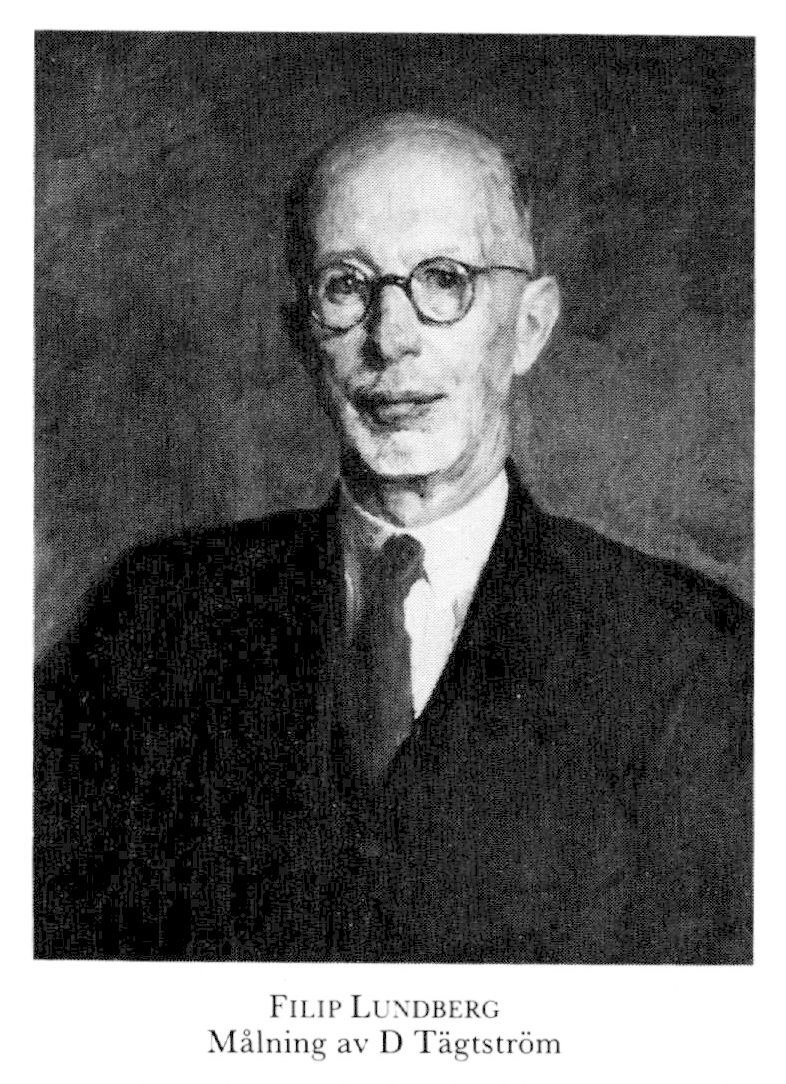
\includegraphics[width=2.21875in,height=\textheight]{Filip_Lundberg.jpg}

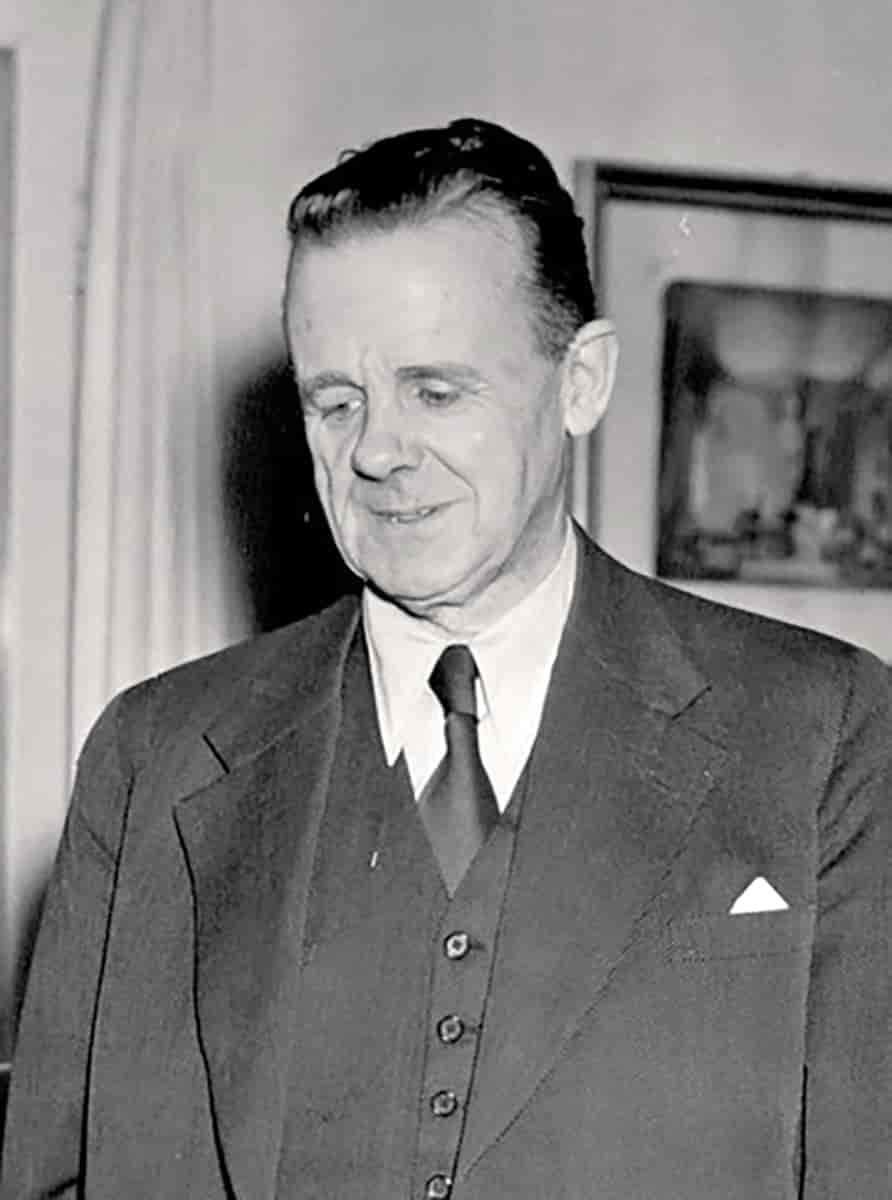
\includegraphics[width=2.23958in,height=\textheight]{harald-cramr.jpg}

En términos más técnicos, el \textbf{modelo de Cramér-Lundberg} se
utiliza para estudiar la \textbf{probabilidad de ruina} de una compañía
de seguros. Aquí están algunos conceptos clave:

\begin{enumerate}
\def\labelenumi{\arabic{enumi}.}
\item
  \textbf{Proceso de Riesgo Clásico}: El capital de la compañía se
  modela como un \textbf{proceso de riesgo}, donde las primas ingresan y
  las reclamaciones salen. La probabilidad de ruina se refiere al riesgo
  de que la compañía no pueda cumplir con sus obligaciones debido a
  insuficiencia de capital.
\item
  \textbf{Distribuciones de Reclamaciones}: Se supone que las
  \textbf{distribuciones del tamaño de los reclamos} son de \textbf{cola
  ligera}, lo que significa que las reclamaciones extremadamente grandes
  son poco probables pero pueden tener un impacto significativo en la
  solvencia de la compañía.
\item
  \textbf{Fórmulas Exactas y Aproximadas}: Se han desarrollado
  \textbf{métodos} para obtener \textbf{fórmulas exactas y aproximadas}
  para la probabilidad de ruina en este modelo. Estas fórmulas permiten
  estimar la posibilidad de que la compañía quiebre debido a pérdidas
  inesperadas.
\item
  \textbf{Simulaciones y Estimaciones}: Además de las fórmulas, se
  realizan \textbf{simulaciones} de las trayectorias del proceso de
  riesgo para diferentes niveles de capital inicial. Esto proporciona
  una perspectiva más completa de las características operativas de la
  aseguradora .
\end{enumerate}

En resumen, el \textbf{modelo de Cramér-Lundberg} es una herramienta
valiosa para evaluar el riesgo financiero en el ámbito de las compañías
de seguros y comprender las posibilidades de ruina en función de las
fluctuaciones en el capital disponible.

\section{Descripción del modelo}\label{descripciuxf3n-del-modelo}

El modelo de Cramér Lundberg se define enseguida como un cierto tipo de
proceso estocástico a tiempo discreto.

Se modela el numero de reclamaciones como un proceso de Poisson
\((N(t))\) con parámetro \(\lambda t\) donde \(t\geq 0\), las pérdidas
individuales \(X_i\) son variables aleatorias independientes e
idénticamente distribuidas (iii)

\begin{definition}[]\protect\hypertarget{def-1}{}\label{def-1}

~

\begin{enumerate}
\def\labelenumi{\arabic{enumi}.}
\item
  El proceso estocástico a tiempo discreto del monto de reclamaciones se
  define como \(\{(X_k): {k \in \mathbb{N} }\}\), donde las \(X_k\) para
  \(k = 1, 2, ...,\) son variables aleatorias
  (Definición~\ref{def-variable_aleatoria}) no negativas, independientes
  e idénticamente distribuidas y tienen función de distribución común
  \(F\), media finita denotada por \(E[X_k] = \mu\) y varianza
  \(Var(X_k) = \sigma^2 \leq \infty\).
\item
  Los tiempos de reclamación ocurren en instantes aleatorios de tiempo
  denotados por \(T_i\) tales que \[ 0 < T_1 < T_2 < \dotsb\]
\item
  El proceso de ocurrencia de las reclamaciones es el número de
  reclamaciones contingentes en el intervalo \([0,t]\), y se define como
  sigue:
\end{enumerate}

\[N(t) = \sup \{n \geq 1: T_n \leq t  \leq 0\}\] y por convención se
usará \(\sup \ \emptyset = 0\).

\begin{enumerate}
\def\labelenumi{\arabic{enumi}.}
\setcounter{enumi}{3}
\item
  Los tiempos entre llegadas son los tiempos que transcurren entre dos
  reclamaciones sucesivas, los cuales se denotan por
  \[Y_i = T_i \ \ \ Y_k= T_k - T_{k-1}, \ \ \ k = 2,3, \dotsb,\]donde
  las variables aleatorias \(Y_k\) son i.i.d. con distribución
  exponencial y media finita \(E[Y_1] =\frac{1}{\lambda}\).
\item
  La sucesión \(\{(X_k): k \in \mathbb{N}\}\) es independiente de la
  sucesión \(\{(Y_k):k\in \mathbb{N}\}.\)
\end{enumerate}

\end{definition}

\begin{definition}[]\protect\hypertarget{def-2}{}\label{def-2}

El proceso de agregado de siniestros \((S(t))_{t \geq 0}\) de un
portafolio se define como:
\begin{equation}\phantomsection\label{eq-1.2}{S(t):= \left\{ \begin{array}{lcc} \sum_{i=1}^{N(t)} X_i, & si & N(t) > 0, \\ \\ 
0, & si & N(t) = 0. \end{array} \right. }\end{equation} El proceso
\((S(t))_{t\geq0}\) es un proceso de suma parcial aleatoria, que se
obtiene al sustituir el índice determinado \(n\) en la suma
\(S_n = X_1 + \dotsb + X_n\) por la variable aleatoria \(N(t):\)
\[S(t) = X_1 + \dotsb+ X_{N(t)} = S_{N(t)}, \ \ t\geq0,\]que se le
conoce como proceso compuesto. Nótese que cuando
\(Var(X_k) = \sigma^2 < \infty\), el proceso del agregado de siniestros
\((S(t))t\ge0\) comparte varias propiedades con el proceso de una suma
parcial, como las propiedades asintóticas del teorema del límite central
y la ley fuerte de los grandes números.

\end{definition}

\begin{lemma}[]\protect\hypertarget{lem-1}{}\label{lem-1}

El agregado de siniestros \((S(t))\) con \(t \geq 0\) tiene función de
distribución
\begin{equation}\phantomsection\label{eq-1.3}{G_s(x) = P[S(t) \leq x] = \sum_{n=0}^{\infty} e^{-\lambda t}\frac{(\lambda t)^n}{n!}F**(x) \ \ \ t\leq 0, x \leq 0,}\end{equation}
donde \(F^{n*}(x)= P[\sum_{i=q}^{n} X_i \leq x]\) es la n-ésima
convolución de F.

\end{lemma}

\begin{proof}
By induction.
\end{proof}

\begin{lemma}[]\protect\hypertarget{lem-2}{}\label{lem-2}

Para cada \(r \geq 0\), el proceso del agregado de siniestros
\((S(t))_{t \geq 0}\) tiene función generadora de momentos
\begin{equation}\phantomsection\label{eq-1.5}{M_{S(t)}(r) = E[e^{rS(t))}] = M_{N(t)}(ln M_{x_i}(r)).}\end{equation}

\end{lemma}

\begin{proof}
By induction.
\end{proof}

El proceso de riesgo \(((U(t))_{t \geq 0}\) se define como sigue:
\begin{equation}\phantomsection\label{eq-1.7}{U(t) = u + ct - S(t) \ \ \ t\geq 0, }\end{equation}
en donde \(u \geq 0\) denota el capital inicial, ct el ingreso vía prima
durante el periodo \([0,t]\) a una tasa constante \(c > 0\) y \(S(t)\)
es el agregado de siniestros en el momento t.

\begin{proposition}[]\protect\hypertarget{prp-1}{}\label{prp-1}

Para cada \(r\geq0\), el proceso de riesgo \((U(t))_{t\geq0}\) tiene
función generadora de momentos
\begin{equation}\phantomsection\label{eq-1.8}{M_{U(t)}(r) =e^{r(u + ct)} M_{S(t)}(-r).}\end{equation}

\end{proposition}

Sea \((U(t))_{t\geq0}\) un proceso de riesgo, entonces para el modelo de
renovación se tiene que: \[E[U(t)] = u + ct - \mu E[N(t)],\] y para el
modelo clásico de Crámer-Lundberg es:
\[E[U(t)] = u + ct - \lambda \mu t.\]

\begin{proof}
By induction.
\end{proof}

\begin{lemma}[]\protect\hypertarget{lem-4}{}\label{lem-4}

Sea \((U(t))_{t\geq0}\)un proceso de riesgo, entonces para el modelo de
renovación se tiene que :
\[ Var(U(t)) = \mu^2 Var(N(t)) + \sigma^2 E[N(t)],\] y para el modelo
clásico Cramér-Lundberg es: \[Var(U(t)) = \lambda t(\sigma^2 + \mu^2).\]

\end{lemma}

\begin{proof}
By induction.
\end{proof}

\bookmarksetup{startatroot}

\chapter{Estudio de caso: Análisis de ventas de una empresa de comida
rápida}\label{estudio-de-caso-anuxe1lisis-de-ventas-de-una-empresa-de-comida-ruxe1pida}

\section{Descripción del problema}\label{descripciuxf3n-del-problema}

Se presentan datos que son parte de las ventas de una empresa de comida
rápida. Para brindar una mejor idea del estudio caso se presentará una
extensión de lo que es una empresa de comida rápida y una franquicia .

Una empresa de comida rápida es un tipo de negocio dentro del sector
alimenticio que se especializa en la preparación y venta de alimentos y
bebidas que pueden ser servidos y consumidos rápidamente. Estas empresas
suelen ofrecer menús estandarizados y utilizan métodos de producción en
masa para asegurar la rapidez y la eficiencia en el servicio. Algunas
características típicas de una empresa de comida rápida incluyen:

1-Rapidez en el Servicio: La principal característica es la rapidez con
la que los clientes pueden recibir sus pedidos, generalmente en pocos
minutos.

2-Menú Limitado y Estandarizado: Los menús suelen ser simples y
consistentes en todas las ubicaciones de la cadena, permitiendo una
preparación rápida y eficiente.

3-Precios Asequibles: Los precios suelen ser más bajos en comparación
con los restaurantes tradicionales, lo que los hace accesibles a una
amplia gama de clientes.

4-Métodos de Preparación Eficientes: Utilizan técnicas de cocción
rápida, como freidoras y parrillas de alta eficiencia, así como la
pre-preparación de ingredientes.

5-Autoservicio y Comida para Llevar: Muchas de estas empresas ofrecen
opciones de autoservicio y comida para llevar, facilitando el consumo
rápido y conveniente.

6-Ambiente Informal: El ambiente es generalmente informal y está
diseñado para facilitar el flujo rápido de clientes, con áreas de
autoservicio y estaciones de recolección de pedidos.

Ejemplos de empresas de comida rápida incluyen grandes cadenas
internacionales como McDonald's, Burger King, KFC, Subway, Carl's Jr y
Taco Bell. Estas empresas han expandido su presencia globalmente,
adaptándose a diferentes mercados y culturas mientras mantienen su
enfoque en la rapidez y eficiencia del servicio.

Muchas de estas empresas otorga parte del derecho a operar en diferentes
franquicias.

Una franquicia es un modelo de negocio en el cual una empresa (el
franquiciador) otorga a otra parte (el franquiciado) el derecho a operar
un negocio utilizando su marca, productos, servicios y modelo operativo
a cambio de una tarifa o regalías. Este modelo permite a los
franquiciadores expandir su marca y presencia en el mercado sin tener
que invertir en nuevas ubicaciones directamente. Al mismo tiempo, ofrece
a los franquiciados la oportunidad de operar un negocio con una marca
establecida y un sistema probado. Algunas características clave de una
franquicia incluyen:

1-Marca y Sistema Operativo: El franquiciado utiliza la marca comercial,
logotipos, productos y servicios del franquiciador, así como su sistema
operativo, que puede incluir recetas, métodos de producción, estrategias
de marketing, entre otros.

2-Pago de Tarifas: El franquiciado paga al franquiciador una tarifa
inicial y, en muchos casos, regalías continuas basadas en un porcentaje
de las ventas. Estas tarifas cubren el uso de la marca y el soporte
continuo del franquiciador.

3-Capacitación y Soporte: El franquiciador proporciona capacitación
inicial y soporte continuo al franquiciado, lo cual puede incluir
formación en gestión empresarial, operaciones, marketing y servicio al
cliente.

4-Estándares y Control de Calidad: Para mantener la consistencia y
calidad de la marca, el franquiciador establece estándares y
procedimientos que los franquiciados deben seguir. Esto puede incluir
auditorias y evaluaciones periódicas.

5-Contrato de Franquicia: La relación entre el franquiciador y el
franquiciado está regulada por un contrato de franquicia que detalla los
derechos y obligaciones de ambas partes, incluyendo la duración del
acuerdo y las condiciones de renovación.

6-Territorio Exclusivo: A menudo, el contrato otorga al franquiciado un
territorio exclusivo en el cual puede operar, evitando la competencia
directa con otras franquicias de la misma marca en esa área.

Ejemplos de negocios que utilizan el modelo de franquicia incluyen
cadenas de comida rápida (como McDonald's, Subway y KFC), Carl's Jr,
hoteles (como Marriott y Hilton), servicios de limpieza, tiendas de
conveniencia y muchos otros sectores. Este modelo permite una expansión
rápida y eficiente del negocio mientras ofrece a los emprendedores la
oportunidad de operar con el respaldo de una marca establecida.

Esta empresa ofrece en sus productos dos tipos de hamburguesas, bebidas
como sodas, cervezas y cafés. En la información de las ventas incluye
registros obtenidos por una Terminal Punto de Venta (TPV), el sistema de
pago usado en establecimientos comerciales para procesar transacciones
de venta. Permite a los comerciantes aceptar el uso de tarjetas de
crédito y débito. Se tiene registro de las ventas por cada día desde el
año 2018 al noviembre del 2020, haciendo un cierre pandémico, se
registran en dos etapas, antes de pandemia los datos a partir del 25 de
julio del 2018 al 10 de abril del 2020. Los datos después de pandemia se
registraron a partir del 3 de agosto del 2020 y cerrando finalmente el
10 de noviembre del 2020, los cuales se les aplicó una homogenización
para un buen manejo de los datos y así poder presentar un mejor
análisis.

\section{Elementos de Ciencia de
Datos}\label{elementos-de-ciencia-de-datos}

\subsection{Importación de los datos originales a
R}\label{importaciuxf3n-de-los-datos-originales-a-r}

Se cargan los datos del archivo excel para ser leído y almacenarlo en un
dataframe (Sección~\ref{sec-dataframe}) para poder manipular cada uno de
los elementos de la base de datos.

\begin{Shaded}
\begin{Highlighting}[]
\NormalTok{Datos }\OtherTok{\textless{}{-}} \FunctionTok{read\_excel}\NormalTok{(}\StringTok{"\textasciitilde{}/TM/Datos.xlsx"}\NormalTok{, }\AttributeTok{col\_types =} 
                  \FunctionTok{c}\NormalTok{(}\StringTok{"numeric"}\NormalTok{,}\StringTok{"numeric"}\NormalTok{,}\StringTok{"numeric"}\NormalTok{,}\StringTok{"numeric"}\NormalTok{,}\StringTok{"numeric"}\NormalTok{,}
                    \StringTok{"numeric"}\NormalTok{,}\StringTok{"numeric"}\NormalTok{,}\StringTok{"numeric"}\NormalTok{,}\StringTok{"numeric"}\NormalTok{,}\StringTok{"numeric"}\NormalTok{, }
                    \StringTok{"numeric"}\NormalTok{,}\StringTok{"numeric"}\NormalTok{,}\StringTok{"numeric"}\NormalTok{,}\StringTok{"numeric"}\NormalTok{,}\StringTok{"numeric"}\NormalTok{, }
                    \StringTok{"numeric"}\NormalTok{,}\StringTok{"numeric"}\NormalTok{,}\StringTok{"numeric"}\NormalTok{,}\StringTok{"numeric"}\NormalTok{,}\StringTok{"numeric"}\NormalTok{, }
                    \StringTok{"numeric"}\NormalTok{,}\StringTok{"numeric"}\NormalTok{,}\StringTok{"numeric"}\NormalTok{,}\StringTok{"numeric"}\NormalTok{,}\StringTok{"numeric"}\NormalTok{, }
                    \StringTok{"numeric"}\NormalTok{,}\StringTok{"numeric"}\NormalTok{,}\StringTok{"numeric"}\NormalTok{,}\StringTok{"numeric"}\NormalTok{,}\StringTok{"numeric"}\NormalTok{, }
                    \StringTok{"numeric"}\NormalTok{,}\StringTok{"numeric"}\NormalTok{,}\StringTok{"numeric"}\NormalTok{,}\StringTok{"numeric"}\NormalTok{,}\StringTok{"numeric"}\NormalTok{, }
                    \StringTok{"numeric"}\NormalTok{,}\StringTok{"numeric"}\NormalTok{,}\StringTok{"numeric"}\NormalTok{,}\StringTok{"numeric"}\NormalTok{,}\StringTok{"numeric"}\NormalTok{, }
                    \StringTok{"numeric"}\NormalTok{,}\StringTok{"numeric"}\NormalTok{,}\StringTok{"numeric"}\NormalTok{,}\StringTok{"numeric"}\NormalTok{,}\StringTok{"numeric"}\NormalTok{,}
                    \StringTok{"numeric"}\NormalTok{,}\StringTok{"numeric"}\NormalTok{,}\StringTok{"numeric"}\NormalTok{,}\StringTok{"numeric"}\NormalTok{,}\StringTok{"numeric"}\NormalTok{, }
                    \StringTok{"numeric"}\NormalTok{,}\StringTok{"numeric"}\NormalTok{,}\StringTok{"numeric"}\NormalTok{,}\StringTok{"numeric"}\NormalTok{,}\StringTok{"numeric"}\NormalTok{, }
                    \StringTok{"numeric"}\NormalTok{,}\StringTok{"numeric"}\NormalTok{,}\StringTok{"numeric"}\NormalTok{,}\StringTok{"numeric"}\NormalTok{,}\StringTok{"numeric"}\NormalTok{, }
                    \StringTok{"numeric"}\NormalTok{,}\StringTok{"numeric"}\NormalTok{,}\StringTok{"numeric"}\NormalTok{,}\StringTok{"numeric"}\NormalTok{,}\StringTok{"numeric"}\NormalTok{, }
                    \StringTok{"numeric"}\NormalTok{,}\StringTok{"numeric"}\NormalTok{,}\StringTok{"numeric"}\NormalTok{,}\StringTok{"numeric"}\NormalTok{,}\StringTok{"numeric"}\NormalTok{, }
                    \StringTok{"numeric"}\NormalTok{,}\StringTok{"numeric"}\NormalTok{,}\StringTok{"numeric"}\NormalTok{,}\StringTok{"numeric"}\NormalTok{,}\StringTok{"numeric"}
\NormalTok{                        ))}

\NormalTok{Datos}
\end{Highlighting}
\end{Shaded}

\begin{verbatim}
# A tibble: 2,416 x 75
    ...1  ...2  ...3  ...4  ...5  ...6 `240519` `82253.5` `247172.9` ...10 `973`
   <dbl> <dbl> <dbl> <dbl> <dbl> <dbl>    <dbl>     <dbl>      <dbl> <dbl> <dbl>
 1    NA    NA    NA    NA    NA    NA      NA        NA         NA     NA   NA 
 2    NA    NA    NA    NA    NA    NA    9382.     9441.        NA     NA 9382.
 3  2018     7    30     4 43306    NA  188038.       NA     188038.    NA  682 
 4  2018     7    30     5 43307    NA  220827        NA     220827     NA  694 
 5  2018     7    30     6 43308    NA  240519        NA     240519     NA  762 
 6  2018     7    30     7 43309    NA  229542        NA     229542     NA  704 
 7  2018     7    30     1 43310    NA  239776.       NA     239776.    NA  706 
 8  2018     7    31     2 43311    NA  172946        NA     172946     NA  602 
 9  2018     7    31     3 43312    NA  210671        NA     210671     NA  709 
10  2018     8    31     4 43313    NA  195662        NA     195662     NA  649 
# i 2,406 more rows
# i 64 more variables: `384` <dbl>, `1136` <dbl>, ...14 <dbl>,
#   `371.753114754098` <dbl>, `2428.16666666666` <dbl>, ...17 <dbl>,
#   ...18 <dbl>, `2099` <dbl>, `222` <dbl>, `2162` <dbl>, ...22 <dbl>,
#   `1384...23` <dbl>, `559` <dbl>, `1384...25` <dbl>, ...26 <dbl>,
#   `2402` <dbl>, `658` <dbl>, `2525` <dbl>, ...30 <dbl>, `1556...31` <dbl>,
#   `462` <dbl>, `1556...33` <dbl>, ...34 <dbl>, `61` <dbl>, `57` <dbl>, ...
\end{verbatim}

Como se puede apreciar, es necesario eliminar columnas, reducido a las
columnas de las ventas de los diferentes productos que oferta la empresa
para así obtener las ventas totales.

\subsection{Homogenización del total de ventas por
día}\label{homogenizaciuxf3n-del-total-de-ventas-por-duxeda}

Mediante este proceso se eliminan y se corrigen valores atípicos,
valores faltantes o alguna inconsistencia que se presentan en los datos.
Esto implica la eliminación de datos incompletos, conocidos como datos
faltantes o NA. También se renombran cabeceras de cada columna del
dataframe para facilitar la lectura del archivo.

\begin{Shaded}
\begin{Highlighting}[]
\CommentTok{\#Eliminamos las columnas con datos faltantes}
\NormalTok{datos }\OtherTok{\textless{}{-}}\NormalTok{ Datos[, }\SpecialCharTok{{-}}\FunctionTok{c}\NormalTok{(}\DecValTok{6}\NormalTok{,}\DecValTok{8}\NormalTok{,}\DecValTok{10}\NormalTok{,}\DecValTok{12}\NormalTok{,}\DecValTok{14}\NormalTok{,}\DecValTok{16}\NormalTok{,}\DecValTok{18}\NormalTok{,}\DecValTok{20}\NormalTok{,}\DecValTok{22}\NormalTok{,}\DecValTok{24}\NormalTok{, }\DecValTok{26}\NormalTok{,}\DecValTok{28}\NormalTok{, }\DecValTok{30}\NormalTok{,}\DecValTok{32}\NormalTok{, }\DecValTok{34}\NormalTok{, }\DecValTok{36}\NormalTok{,}
                    \DecValTok{38}\NormalTok{,}\DecValTok{39}\NormalTok{, }\DecValTok{40}\NormalTok{,  }\DecValTok{42}\NormalTok{, }\DecValTok{44}\NormalTok{, }\DecValTok{46}\NormalTok{, }\DecValTok{48}\NormalTok{, }\DecValTok{50}\NormalTok{,}\DecValTok{51}\NormalTok{,}\DecValTok{52}\NormalTok{, }\DecValTok{53}\NormalTok{, }\DecValTok{54}\NormalTok{,}\DecValTok{55}\NormalTok{, }\DecValTok{56}\NormalTok{, }
\DecValTok{57}\NormalTok{,}\DecValTok{58}\NormalTok{,}\DecValTok{59}\NormalTok{,}\DecValTok{60}\NormalTok{,}\DecValTok{61}\NormalTok{, }\DecValTok{62}\NormalTok{, }\DecValTok{63}\NormalTok{, }\DecValTok{64}\NormalTok{, }\DecValTok{65}\NormalTok{, }\DecValTok{66}\NormalTok{, }\DecValTok{67}\NormalTok{, }\DecValTok{68}\NormalTok{, }\DecValTok{69}\NormalTok{, }\DecValTok{70}\NormalTok{, }\DecValTok{71}\NormalTok{, }\DecValTok{73}\NormalTok{,}\DecValTok{74}\NormalTok{,}\DecValTok{72}\NormalTok{, }\DecValTok{75}\NormalTok{)]}
\CommentTok{\#Cambiar las cabeceras del dataframe  }
\NormalTok{datos }\OtherTok{\textless{}{-}} \FunctionTok{data.frame}\NormalTok{(datos}\SpecialCharTok{\%\textgreater{}\%} \FunctionTok{rename}\NormalTok{(Año }\OtherTok{=}\NormalTok{ ...}\DecValTok{1}\NormalTok{ ))}
\NormalTok{datos }\OtherTok{\textless{}{-}} \FunctionTok{data.frame}\NormalTok{(datos}\SpecialCharTok{\%\textgreater{}\%} \FunctionTok{rename}\NormalTok{(}\AttributeTok{Mes =}\NormalTok{ ...}\DecValTok{2}\NormalTok{, }\AttributeTok{Semana =}\NormalTok{ ...}\DecValTok{3}\NormalTok{, }\AttributeTok{Dia=}\NormalTok{ ...}\DecValTok{4}\NormalTok{, }
                  \AttributeTok{Fecha =}\NormalTok{ ...}\DecValTok{5}\NormalTok{, }\AttributeTok{Ventas=}\NormalTok{ X240519, }
                  \AttributeTok{TotalVentas =}\NormalTok{ X247172}\FloatTok{.9}\NormalTok{,}\AttributeTok{Customers =}\NormalTok{ X973,}
                  \AttributeTok{Totalcustomers =}\NormalTok{ X1136, }
                  \AttributeTok{CH\_Promedio =}\NormalTok{ X371}\FloatTok{.753114754098}\NormalTok{, }
                  \AttributeTok{TotalCH\_Promedio =}\NormalTok{ ...}\DecValTok{17}\NormalTok{, }\AttributeTok{Burgers =}\NormalTok{ X2099,}
                  \AttributeTok{TotalBurgers =}\NormalTok{ X2162, }
                  \AttributeTok{Thickurgers =}\NormalTok{ X1384...}\DecValTok{23}\NormalTok{, }
                  \AttributeTok{TotalThickburgers =}\NormalTok{ X1384...}\DecValTok{25}\NormalTok{,}
                  \AttributeTok{Total\_Burgers =}\NormalTok{ X2402, }
                  \AttributeTok{T\_Total\_Burgers=}\NormalTok{ X2525,}\AttributeTok{Bebidas =}\NormalTok{ X1556...}\DecValTok{31}\NormalTok{,}
                  \AttributeTok{Totalbebidas =}\NormalTok{ X1556...}\DecValTok{33}\NormalTok{, }\AttributeTok{Cervezas =}\NormalTok{ X61,}
                  \AttributeTok{Totalcervezas =}\NormalTok{ X83, }\AttributeTok{Cafes =}\NormalTok{ X83,}
                  \AttributeTok{Totalcafes =}\NormalTok{ X54, }\AttributeTok{Ventas\_TPV =}\NormalTok{ X158904,}
                  \AttributeTok{Total\_Ventas\_TPV =}\NormalTok{ X173412}\FloatTok{.5}\NormalTok{,}
                  \AttributeTok{HR\_Laborales =}\NormalTok{ ...}\DecValTok{47}\NormalTok{,}
                  \AttributeTok{Total\_HR\_Laborales =}\NormalTok{ ...}\DecValTok{49}\NormalTok{ ))}
\end{Highlighting}
\end{Shaded}

Por último, se realizó la separación de la base de datos antes de la
pandemia y después de la pandemia, presentando así los dataframes
resultantes en el siguiente código y como se ilustra posteriormente:

\begin{Shaded}
\begin{Highlighting}[]
\CommentTok{\#Analisis de los datos:}
\CommentTok{\#Filtros por días:}
\CommentTok{\#\_\_\_\_\_\_\_\_\_\_\_\_\_\_\_\_\_\_\_\_\_\_\_\_\_\_\_Antes de la pandemia\_\_\_\_\_\_\_\_\_\_\_\_\_\_\_\_\_\_\_\_\_\_\_\_\_\_\_}

\NormalTok{fil\_before1}\OtherTok{\textless{}{-}} \FunctionTok{data.frame}\NormalTok{(}\FunctionTok{subset}\NormalTok{(datos, Año }\SpecialCharTok{\textless{}=} \DecValTok{2019}\NormalTok{))}
\NormalTok{fil\_before2}\OtherTok{\textless{}{-}} \FunctionTok{data.frame}\NormalTok{(}\FunctionTok{subset}\NormalTok{(datos, Año }\SpecialCharTok{==} \DecValTok{2020} \SpecialCharTok{\&}\NormalTok{ Mes }\SpecialCharTok{\textless{}=} \DecValTok{4}\NormalTok{))}
\NormalTok{fil\_before }\OtherTok{\textless{}{-}} \FunctionTok{rbind}\NormalTok{(fil\_before1, fil\_before2)}

\CommentTok{\#\_\_\_\_\_\_\_\_\_\_\_\_\_\_\_\_\_\_\_\_\_\_\_\_Después de la pandemia\_\_\_\_\_\_\_\_\_\_\_\_\_\_\_\_\_\_\_\_\_\_\_\_\_\_\_\_}

\NormalTok{fil\_dat\_after }\OtherTok{\textless{}{-}} \FunctionTok{data.frame}\NormalTok{(}\FunctionTok{subset}\NormalTok{(datos, Año }\SpecialCharTok{==} \DecValTok{2020} \SpecialCharTok{\&}\NormalTok{ Mes}\SpecialCharTok{\textgreater{}=}\DecValTok{8}\NormalTok{))}
\end{Highlighting}
\end{Shaded}

\subsection{DataFrame Resultante: Antes de la
pandemia}\label{dataframe-resultante-antes-de-la-pandemia}

\begin{verbatim}
    Año Mes Dia   Ventas TotalVentas
3  2018   7   4 188037.5    188037.5
4  2018   7   5 220827.0    220827.0
5  2018   7   6 240519.0    240519.0
6  2018   7   7 229542.0    229542.0
7  2018   7   1 239775.6    239775.6
8  2018   7   2 172946.0    172946.0
9  2018   7   3 210671.0    210671.0
10 2018   8   4 195662.0    195662.0
11 2018   8   5 193051.0    193051.0
12 2018   8   6 206803.0    206803.0
13 2018   8   7 219399.0    219399.0
14 2018   8   1 224106.5    224106.5
15 2018   8   2 152557.0    152557.0
16 2018   8   3 148675.5    148675.5
17 2018   8   4 142344.0    142344.0
18 2018   8   5 152189.5    152189.5
19 2018   8   6 171891.0    171891.0
20 2018   8   7 194642.5    194642.5
21 2018   8   1 210023.5    210023.5
22 2018   8   2 129751.5    129751.5
23 2018   8   3 125867.5    125867.5
24 2018   8   4 133380.0    133380.0
25 2018   8   5 135070.5    135070.5
26 2018   8   6 158927.0    158927.0
27 2018   8   7 175382.0    175382.0
28 2018   8   1 187502.0    187502.0
29 2018   8   2  78116.0     78116.0
30 2018   8   3  71871.0     71871.0
31 2018   8   4  82471.5     82471.5
32 2018   8   5  98739.5     98739.5
33 2018   8   6 131185.5    131185.5
34 2018   8   7 157909.5    157909.5
35 2018   8   1 186582.0    186582.0
36 2018   8   2  68030.0     68030.0
37 2018   8   3  71887.0     71887.0
38 2018   8   4  74843.5     74843.5
39 2018   8   5  77880.5     77880.5
40 2018   8   6 128575.0    128575.0
\end{verbatim}

\subsection{DataFrame Resultante: Después de la
pandemia}\label{dataframe-resultante-despuuxe9s-de-la-pandemia}

\begin{verbatim}
     Año Mes Dia    Ventas TotalVentas
743 2020   8   2  44908.70    53887.70
744 2020   8   3  51733.00    69538.00
745 2020   8   4  57876.95    57876.95
746 2020   8   5  47554.60    57540.10
747 2020   8   6  67138.20    70025.20
748 2020   8   7  89172.70    99932.70
749 2020   8   1 113384.70   130996.70
750 2020   8   2  40974.60    47464.60
751 2020   8   3  48520.10    57037.10
752 2020   8   4  46649.15    52529.65
753 2020   8   5  40556.90    51963.40
754 2020   8   6  70159.10    81004.10
755 2020   8   7  77736.80    89482.30
756 2020   8   1 107918.30   120988.30
757 2020   8   2  48885.80    59032.80
758 2020   8   3  48311.20    57724.70
759 2020   8   4  44658.00    46319.00
760 2020   8   5  63104.30    69302.80
761 2020   8   6  67481.30    76436.30
762 2020   8   7  89795.30   102998.80
763 2020   8   1 102744.90   118060.90
764 2020   8   2  34713.50    42455.00
765 2020   8   3  40403.40    53956.40
766 2020   8   4  47028.10    56991.10
767 2020   8   5  31703.55    45095.55
768 2020   8   6  59907.40    75201.90
769 2020   8   7  89533.40    98554.40
770 2020   8   1 103271.20   115973.20
771 2020   8   2  47309.40    59826.40
\end{verbatim}

Para realizar la identificación de las diferentes distribuciones e
implementar los gráficos como los histogramas y los boxplot, se elaboran
filtros correspondientes para las ventas por cada día antes y después de
pandemia

Los comandos para realizar los filtros es el siguiente:

\begin{Shaded}
\begin{Highlighting}[]
\CommentTok{\#filtra los datos del día Domingo antes de la pandemia}
\NormalTok{fil\_dat\_1\_before}\OtherTok{\textless{}{-}} \FunctionTok{data.frame}\NormalTok{(}\FunctionTok{subset}\NormalTok{(fil\_before, Dia }\SpecialCharTok{==} \DecValTok{1}\NormalTok{))}
\CommentTok{\#\_\_\_\_\_\_\_\_\_\_\_\_\_\_\_\_\_\_\_\_\_\_\_\_\_\_\_\_\_\_\_\_\_\_\_\_\_\_\_\_\_\_\_\_\_\_\_\_\_\_\_\_\_\_\_\_\_\_\_}
\CommentTok{\#filtra los datos del día Lunes antes de la pandemia}
\NormalTok{fil\_dat\_2\_before}\OtherTok{\textless{}{-}} \FunctionTok{data.frame}\NormalTok{(}\FunctionTok{subset}\NormalTok{(fil\_before, Dia }\SpecialCharTok{==} \DecValTok{2}\NormalTok{))}
\CommentTok{\#\_\_\_\_\_\_\_\_\_\_\_\_\_\_\_\_\_\_\_\_\_\_\_\_\_\_\_\_\_\_\_\_\_\_\_\_\_\_\_\_\_\_\_\_\_\_\_\_\_\_\_\_\_\_\_\_\_\_\_}
\CommentTok{\#filtra los datos del día martes antes de la pandemia}
\NormalTok{fil\_dat\_3\_before}\OtherTok{\textless{}{-}} \FunctionTok{data.frame}\NormalTok{(}\FunctionTok{subset}\NormalTok{(fil\_before, Dia }\SpecialCharTok{==} \DecValTok{3}\NormalTok{))}
\CommentTok{\#\_\_\_\_\_\_\_\_\_\_\_\_\_\_\_\_\_\_\_\_\_\_\_\_\_\_\_\_\_\_\_\_\_\_\_\_\_\_\_\_\_\_\_\_\_\_\_\_\_\_\_\_\_\_\_\_\_\_\_}
\CommentTok{\#filtra los datos del día miércoles antes de la pandemia}
\NormalTok{fil\_dat\_4\_before}\OtherTok{\textless{}{-}} \FunctionTok{data.frame}\NormalTok{(}\FunctionTok{subset}\NormalTok{(fil\_before, Dia }\SpecialCharTok{==} \DecValTok{4}\NormalTok{))}
\CommentTok{\#\_\_\_\_\_\_\_\_\_\_\_\_\_\_\_\_\_\_\_\_\_\_\_\_\_\_\_\_\_\_\_\_\_\_\_\_\_\_\_\_\_\_\_\_\_\_\_\_\_\_\_\_\_\_\_\_\_\_\_}
\CommentTok{\#filtra los datos del día Jueves antes de la pandemia}
\NormalTok{fil\_dat\_5\_before}\OtherTok{\textless{}{-}} \FunctionTok{data.frame}\NormalTok{(}\FunctionTok{subset}\NormalTok{(fil\_before, Dia }\SpecialCharTok{==} \DecValTok{5}\NormalTok{))}
\CommentTok{\#\_\_\_\_\_\_\_\_\_\_\_\_\_\_\_\_\_\_\_\_\_\_\_\_\_\_\_\_\_\_\_\_\_\_\_\_\_\_\_\_\_\_\_\_\_\_\_\_\_\_\_\_\_\_\_\_\_\_\_}
\CommentTok{\#filtra los datos del día Viernes antes de la pandemia}
\NormalTok{fil\_dat\_6\_before}\OtherTok{\textless{}{-}} \FunctionTok{data.frame}\NormalTok{(}\FunctionTok{subset}\NormalTok{(fil\_before, Dia }\SpecialCharTok{==} \DecValTok{6}\NormalTok{))}
\CommentTok{\#\_\_\_\_\_\_\_\_\_\_\_\_\_\_\_\_\_\_\_\_\_\_\_\_\_\_\_\_\_\_\_\_\_\_\_\_\_\_\_\_\_\_\_\_\_\_\_\_\_\_\_\_\_\_\_\_\_\_\_}
\CommentTok{\#filtra los datos del día Sábado antes de la pandemia}
\NormalTok{fil\_dat\_7\_before}\OtherTok{\textless{}{-}} \FunctionTok{data.frame}\NormalTok{(}\FunctionTok{subset}\NormalTok{(fil\_before, Dia }\SpecialCharTok{==} \DecValTok{7}\NormalTok{))}
\end{Highlighting}
\end{Shaded}

\begin{Shaded}
\begin{Highlighting}[]
\CommentTok{\#\_\_\_\_\_\_\_\_\_\_\_\_\_\_\_\_\_\_\_\_\_\_\_\_\_\_\_\_\_\_\_\_\_\_\_\_\_\_\_\_\_\_\_\_\_\_\_\_\_\_\_\_\_\_\_\_\_\_\_\_\_\_\_\_\_\_\_\_}
\NormalTok{fil\_dat\_after }\OtherTok{\textless{}{-}} \FunctionTok{data.frame}\NormalTok{(}\FunctionTok{subset}\NormalTok{(datos, Año }\SpecialCharTok{==} \DecValTok{2020} \SpecialCharTok{\&}\NormalTok{ Mes}\SpecialCharTok{\textgreater{}=}\DecValTok{8}\NormalTok{))}
\CommentTok{\#filtra los datos del día domingo despues de la pandemia}
\NormalTok{fil\_dat\_1\_after}\OtherTok{\textless{}{-}} \FunctionTok{data.frame}\NormalTok{(}\FunctionTok{subset}\NormalTok{(datos, }
\NormalTok{                                    Año }\SpecialCharTok{==} \DecValTok{2020} \SpecialCharTok{\&}\NormalTok{ Mes }\SpecialCharTok{\textgreater{}=} \DecValTok{8} \SpecialCharTok{\&}\NormalTok{ Dia}\SpecialCharTok{==}\DecValTok{1}\NormalTok{))}
\CommentTok{\#\_\_\_\_\_\_\_\_\_\_\_\_\_\_\_\_\_\_\_\_\_\_\_\_\_\_\_\_\_\_\_\_\_\_\_\_\_\_\_\_\_\_\_\_\_\_\_\_\_\_\_\_\_\_\_\_\_\_\_\_\_\_\_\_\_\_\_\_}
\CommentTok{\#filtra los datos del día lunes despues de la pandemia}
\NormalTok{fil\_dat\_2\_after}\OtherTok{\textless{}{-}} \FunctionTok{data.frame}\NormalTok{(}\FunctionTok{subset}\NormalTok{(datos,}
\NormalTok{                                    Año }\SpecialCharTok{==} \DecValTok{2020} \SpecialCharTok{\&}\NormalTok{ Mes }\SpecialCharTok{\textgreater{}=} \DecValTok{8} \SpecialCharTok{\&}\NormalTok{ Dia }\SpecialCharTok{==}\DecValTok{2}\NormalTok{))}
\CommentTok{\#\_\_\_\_\_\_\_\_\_\_\_\_\_\_\_\_\_\_\_\_\_\_\_\_\_\_\_\_\_\_\_\_\_\_\_\_\_\_\_\_\_\_\_\_\_\_\_\_\_\_\_\_\_\_\_\_\_\_\_\_\_\_\_\_\_\_\_\_}
\CommentTok{\#filtra los datos del día martes despues de la pandemia}
\NormalTok{fil\_dat\_3\_after}\OtherTok{\textless{}{-}} \FunctionTok{data.frame}\NormalTok{(}\FunctionTok{subset}\NormalTok{(datos,}
\NormalTok{                                    Año }\SpecialCharTok{==} \DecValTok{2020} \SpecialCharTok{\&}\NormalTok{ Mes }\SpecialCharTok{\textgreater{}=} \DecValTok{8} \SpecialCharTok{\&}\NormalTok{ Dia }\SpecialCharTok{==}\DecValTok{3}\NormalTok{))}
\CommentTok{\#\_\_\_\_\_\_\_\_\_\_\_\_\_\_\_\_\_\_\_\_\_\_\_\_\_\_\_\_\_\_\_\_\_\_\_\_\_\_\_\_\_\_\_\_\_\_\_\_\_\_\_\_\_\_\_\_\_\_\_\_\_\_\_\_\_\_\_\_}
\CommentTok{\#filtra los datos del día miércoles despues de la pandemia}
\NormalTok{fil\_dat\_4\_after}\OtherTok{\textless{}{-}} \FunctionTok{data.frame}\NormalTok{(}\FunctionTok{subset}\NormalTok{(datos,}
\NormalTok{                                    Año }\SpecialCharTok{==} \DecValTok{2020} \SpecialCharTok{\&}\NormalTok{ Mes }\SpecialCharTok{\textgreater{}=} \DecValTok{8} \SpecialCharTok{\&}\NormalTok{ Dia }\SpecialCharTok{==}\DecValTok{4}\NormalTok{))}
\CommentTok{\#\_\_\_\_\_\_\_\_\_\_\_\_\_\_\_\_\_\_\_\_\_\_\_\_\_\_\_\_\_\_\_\_\_\_\_\_\_\_\_\_\_\_\_\_\_\_\_\_\_\_\_\_\_\_\_\_\_\_\_\_\_\_\_\_\_\_\_\_}
\CommentTok{\#filtra los datos del día jueves despues de la pandemia}
\NormalTok{fil\_dat\_5\_after}\OtherTok{\textless{}{-}} \FunctionTok{data.frame}\NormalTok{(}\FunctionTok{subset}\NormalTok{(datos,}
\NormalTok{                                    Año }\SpecialCharTok{==} \DecValTok{2020} \SpecialCharTok{\&}\NormalTok{ Mes }\SpecialCharTok{\textgreater{}=} \DecValTok{8} \SpecialCharTok{\&}\NormalTok{ Dia }\SpecialCharTok{==}\DecValTok{5}\NormalTok{))}
\CommentTok{\#\_\_\_\_\_\_\_\_\_\_\_\_\_\_\_\_\_\_\_\_\_\_\_\_\_\_\_\_\_\_\_\_\_\_\_\_\_\_\_\_\_\_\_\_\_\_\_\_\_\_\_\_\_\_\_\_\_\_\_\_\_\_\_\_\_\_\_\_}
\CommentTok{\#filtra los datos del día viernes despues de la pandemia}
\NormalTok{fil\_dat\_6\_after}\OtherTok{\textless{}{-}} \FunctionTok{data.frame}\NormalTok{(}\FunctionTok{subset}\NormalTok{(datos,}
\NormalTok{                                    Año }\SpecialCharTok{==} \DecValTok{2020} \SpecialCharTok{\&}\NormalTok{ Mes }\SpecialCharTok{\textgreater{}=} \DecValTok{8} \SpecialCharTok{\&}\NormalTok{ Dia }\SpecialCharTok{==}\DecValTok{6}\NormalTok{))}
\CommentTok{\#\_\_\_\_\_\_\_\_\_\_\_\_\_\_\_\_\_\_\_\_\_\_\_\_\_\_\_\_\_\_\_\_\_\_\_\_\_\_\_\_\_\_\_\_\_\_\_\_\_\_\_\_\_\_\_\_\_\_\_\_\_\_\_\_\_\_\_\_}
\CommentTok{\#filtra los datos del día sábado despues de la pandemia}
\NormalTok{fil\_dat\_7\_after}\OtherTok{\textless{}{-}} \FunctionTok{data.frame}\NormalTok{(}\FunctionTok{subset}\NormalTok{(datos,}
\NormalTok{                                    Año }\SpecialCharTok{==} \DecValTok{2020} \SpecialCharTok{\&}\NormalTok{ Mes }\SpecialCharTok{\textgreater{}=} \DecValTok{8} \SpecialCharTok{\&}\NormalTok{ Dia }\SpecialCharTok{==}\DecValTok{7}\NormalTok{))}
\end{Highlighting}
\end{Shaded}

Para visualizar gráficamente el comportamiento de las ventas por día, a
continuación se construyen los histogramas por día, en los periodos
antes y después de la pandemia.

\subsection{Análisis gráfico de las ventas por
día:}\label{anuxe1lisis-gruxe1fico-de-las-ventas-por-duxeda}

Para la generación de los gráficos se empleó los filtros anteriores, con
el fin de obtener un análisis descriptivo de cada uno de ellos.

\subsubsection{Histogramas de los datos de ventas por día antes de la
pandemia}\label{histogramas-de-los-datos-de-ventas-por-duxeda-antes-de-la-pandemia}

El código que genera estos histogramas en R es el siguiente:

\begin{Shaded}
\begin{Highlighting}[]
\CommentTok{\# muestra el gráfico de todos los histogramas de ventas por día }
\CommentTok{\# antes de la pandemia}
\FunctionTok{par}\NormalTok{(}\AttributeTok{mar=}\FunctionTok{c}\NormalTok{(}\DecValTok{2}\NormalTok{,}\DecValTok{2}\NormalTok{,}\DecValTok{2}\NormalTok{,}\DecValTok{2}\NormalTok{))}
\FunctionTok{par}\NormalTok{(}\AttributeTok{mfrow =}\FunctionTok{c}\NormalTok{(}\DecValTok{3}\NormalTok{,}\DecValTok{3}\NormalTok{))}
\FunctionTok{hist}\NormalTok{(fil\_dat\_1\_before}\SpecialCharTok{$}\NormalTok{Ventas, }
     \AttributeTok{main =} \StringTok{"Ventas día Domingo"}\NormalTok{, }\AttributeTok{xlab =} \StringTok{"Ventas"}\NormalTok{)}
\FunctionTok{hist}\NormalTok{(fil\_dat\_2\_before}\SpecialCharTok{$}\NormalTok{Ventas, }
     \AttributeTok{main =} \StringTok{"Ventas día Lunes"}\NormalTok{, }\AttributeTok{xlab =} \StringTok{"Ventas"}\NormalTok{)}
\FunctionTok{hist}\NormalTok{(fil\_dat\_3\_before}\SpecialCharTok{$}\NormalTok{Ventas,}
     \AttributeTok{main =} \StringTok{"Ventas día Martes"}\NormalTok{, }\AttributeTok{xlab =} \StringTok{"Ventas"}\NormalTok{)}
\FunctionTok{hist}\NormalTok{(fil\_dat\_4\_before}\SpecialCharTok{$}\NormalTok{Ventas, }
     \AttributeTok{main =} \StringTok{"Ventas día Miércoles"}\NormalTok{, }\AttributeTok{xlab =} \StringTok{"Ventas"}\NormalTok{)}
\FunctionTok{hist}\NormalTok{(fil\_dat\_5\_before}\SpecialCharTok{$}\NormalTok{Ventas, }
     \AttributeTok{main =} \StringTok{"Ventas día Jueves"}\NormalTok{, }\AttributeTok{xlab =} \StringTok{"Ventas"}\NormalTok{)}
\FunctionTok{hist}\NormalTok{(fil\_dat\_6\_before}\SpecialCharTok{$}\NormalTok{Ventas, }
     \AttributeTok{main =} \StringTok{"Ventas día Viernes"}\NormalTok{, }\AttributeTok{xlab =} \StringTok{"Ventas"}\NormalTok{)}
\FunctionTok{hist}\NormalTok{(fil\_dat\_7\_before}\SpecialCharTok{$}\NormalTok{Ventas, }
     \AttributeTok{main =} \StringTok{"Ventas día Sábado"}\NormalTok{, }\AttributeTok{xlab =} \StringTok{"Ventas"}\NormalTok{)}
\end{Highlighting}
\end{Shaded}

\begin{figure}[H]

{\centering 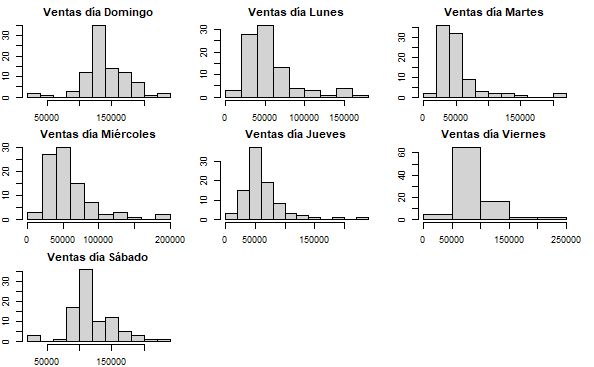
\includegraphics[width=0.8\textwidth,height=\textheight]{his_1.png}

}

\caption{Histogramas de las ventas por día antes de la pandemia.}

\end{figure}%

Para profundizar en el análisis descriptivo de las ventas periódicas se
presenta ahora los boxplot de las ventas por cada día de la semana.

\subsubsection{Boxplot de datos de ventas por días antes de la
pandemia}\label{boxplot-de-datos-de-ventas-por-duxedas-antes-de-la-pandemia}

\begin{verbatim}
   Min. 1st Qu.  Median    Mean 3rd Qu.    Max. 
  30977  122963  135498  138498  158347  239776 
\end{verbatim}

\begin{verbatim}
   Min. 1st Qu.  Median    Mean 3rd Qu.    Max. 
   7430   35919   48676   57388   68030  172946 
\end{verbatim}

\begin{verbatim}
   Min. 1st Qu.  Median    Mean 3rd Qu.    Max. 
  12950   35210   44398   53367   56624  219702 
\end{verbatim}

\begin{verbatim}
   Min. 1st Qu.  Median    Mean 3rd Qu.    Max. 
  10832   35847   44213   56365   63585  195662 
\end{verbatim}

\begin{verbatim}
   Min. 1st Qu.  Median    Mean 3rd Qu.    Max. 
  13547   42368   49479   61068   70047  220827 
\end{verbatim}

\begin{verbatim}
   Min. 1st Qu.  Median    Mean 3rd Qu.    Max. 
  10331   65730   79464   86514   96522  240519 
\end{verbatim}

\begin{verbatim}
   Min. 1st Qu.  Median    Mean 3rd Qu.    Max. 
  24219  100751  110603  119332  135176  229542 
\end{verbatim}

El código que genera en R los boxplot es el siguiente:

\begin{Shaded}
\begin{Highlighting}[]
\CommentTok{\# muestra el gráfico de todos los boxplot de ventas por día }
\CommentTok{\# antes de la pandemia }
\NormalTok{fig }\OtherTok{\textless{}{-}} \FunctionTok{plot\_ly}\NormalTok{(}\AttributeTok{y =}\NormalTok{fil\_dat\_1\_before}\SpecialCharTok{$}\NormalTok{Ventas, }\AttributeTok{name =} \StringTok{"Ventas día Domingo"}\NormalTok{, }
               \AttributeTok{boxpoints =} \StringTok{"all"}\NormalTok{,}\AttributeTok{type =} \StringTok{"box"}\NormalTok{, )}
\NormalTok{fig }\OtherTok{\textless{}{-}}\NormalTok{ fig }\SpecialCharTok{\%\textgreater{}\%} \FunctionTok{add\_trace}\NormalTok{(}\AttributeTok{y =}\NormalTok{ fil\_dat\_2\_before}\SpecialCharTok{$}\NormalTok{Ventas,  }
                         \AttributeTok{name =} \StringTok{"Ventas día Lunes"}\NormalTok{, }\AttributeTok{boxpoints =} \StringTok{"all"}\NormalTok{)}
\NormalTok{fig }\OtherTok{\textless{}{-}}\NormalTok{ fig }\SpecialCharTok{\%\textgreater{}\%} \FunctionTok{add\_trace}\NormalTok{(}\AttributeTok{y =}\NormalTok{ fil\_dat\_3\_before}\SpecialCharTok{$}\NormalTok{Ventas,  }
                         \AttributeTok{name =} \StringTok{"Ventas día Martes"}\NormalTok{, }\AttributeTok{boxpoints =} \StringTok{"all"}\NormalTok{)}
\NormalTok{fig }\OtherTok{\textless{}{-}}\NormalTok{ fig }\SpecialCharTok{\%\textgreater{}\%} \FunctionTok{add\_trace}\NormalTok{(}\AttributeTok{y =}\NormalTok{ fil\_dat\_4\_before}\SpecialCharTok{$}\NormalTok{Ventas,  }
                         \AttributeTok{name =} \StringTok{"Ventas día Miércoles"}\NormalTok{, }\AttributeTok{boxpoints =} \StringTok{"all"}\NormalTok{)}
\NormalTok{fig }\OtherTok{\textless{}{-}}\NormalTok{ fig }\SpecialCharTok{\%\textgreater{}\%} \FunctionTok{add\_trace}\NormalTok{(}\AttributeTok{y =}\NormalTok{ fil\_dat\_5\_before}\SpecialCharTok{$}\NormalTok{Ventas,  }
                         \AttributeTok{name =} \StringTok{"Ventas día Jueves"}\NormalTok{, }\AttributeTok{boxpoints =} \StringTok{"all"}\NormalTok{)}
\NormalTok{fig }\OtherTok{\textless{}{-}}\NormalTok{ fig }\SpecialCharTok{\%\textgreater{}\%} \FunctionTok{add\_trace}\NormalTok{(}\AttributeTok{y =}\NormalTok{ fil\_dat\_6\_before}\SpecialCharTok{$}\NormalTok{Ventas,  }
                         \AttributeTok{name =} \StringTok{"Ventas día Viernes"}\NormalTok{, }\AttributeTok{boxpoints =} \StringTok{"all"}\NormalTok{)}
\NormalTok{fig }\OtherTok{\textless{}{-}}\NormalTok{ fig }\SpecialCharTok{\%\textgreater{}\%} \FunctionTok{add\_trace}\NormalTok{(}\AttributeTok{y =}\NormalTok{ fil\_dat\_7\_before}\SpecialCharTok{$}\NormalTok{Ventas,  }
                         \AttributeTok{name =} \StringTok{"Ventas día Sábado"}\NormalTok{, }\AttributeTok{boxpoints =} \StringTok{"all"}\NormalTok{)}

\NormalTok{fig}
\end{Highlighting}
\end{Shaded}

\begin{figure}[H]

{\centering 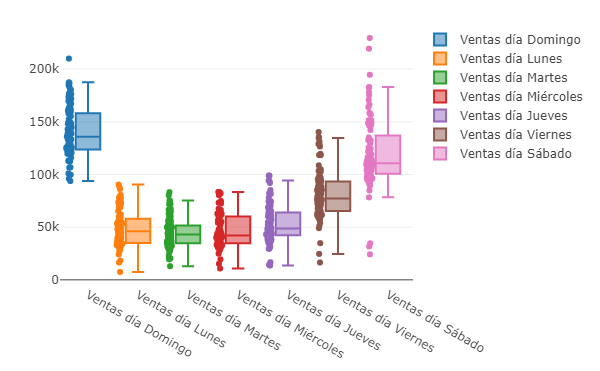
\includegraphics{fig-box1pdf.png}

}

\caption{Boxplot de las ventas por día antes de la pandemia.}

\end{figure}%

\subsubsection{Histogramas de los datos de ventas por día después de la
pandemia}\label{histogramas-de-los-datos-de-ventas-por-duxeda-despuuxe9s-de-la-pandemia}

El código que genera estos histogramas en R es el siguiente:

\begin{Shaded}
\begin{Highlighting}[]
\CommentTok{\# muestra el gráfico de todos los histogramas de ventas por día }
\CommentTok{\#despues de la pandemia}
\FunctionTok{par}\NormalTok{(}\AttributeTok{mar=}\FunctionTok{c}\NormalTok{(}\DecValTok{2}\NormalTok{,}\DecValTok{2}\NormalTok{,}\DecValTok{2}\NormalTok{,}\DecValTok{2}\NormalTok{))}
\FunctionTok{par}\NormalTok{(}\AttributeTok{mfrow =}\FunctionTok{c}\NormalTok{(}\DecValTok{3}\NormalTok{,}\DecValTok{3}\NormalTok{))}
\FunctionTok{hist}\NormalTok{(fil\_dat\_1\_after}\SpecialCharTok{$}\NormalTok{Ventas, }
     \AttributeTok{main =} \StringTok{"Ventas día Domingo"}\NormalTok{, }\AttributeTok{xlab =} \StringTok{"Ventas"}\NormalTok{)}
\FunctionTok{hist}\NormalTok{(fil\_dat\_2\_after}\SpecialCharTok{$}\NormalTok{Ventas, }
     \AttributeTok{main =} \StringTok{"Ventas día Lunes"}\NormalTok{, }\AttributeTok{xlab =} \StringTok{"Ventas"}\NormalTok{)}
\FunctionTok{hist}\NormalTok{(fil\_dat\_3\_after}\SpecialCharTok{$}\NormalTok{Ventas, }
     \AttributeTok{main =} \StringTok{"Ventas día Martes"}\NormalTok{, }\AttributeTok{xlab =} \StringTok{"Ventas"}\NormalTok{)}
\FunctionTok{hist}\NormalTok{(fil\_dat\_4\_after}\SpecialCharTok{$}\NormalTok{Ventas,}
     \AttributeTok{main =} \StringTok{"Ventas día Miércoles"}\NormalTok{, }\AttributeTok{xlab =} \StringTok{"Ventas"}\NormalTok{)}
\FunctionTok{hist}\NormalTok{(fil\_dat\_5\_after}\SpecialCharTok{$}\NormalTok{Ventas, }
     \AttributeTok{main =} \StringTok{"Ventas día Jueves"}\NormalTok{, }\AttributeTok{xlab =} \StringTok{"Ventas"}\NormalTok{)}
\FunctionTok{hist}\NormalTok{(fil\_dat\_6\_after}\SpecialCharTok{$}\NormalTok{Ventas, }
     \AttributeTok{main =} \StringTok{"Ventas día Viernes"}\NormalTok{, }\AttributeTok{xlab =} \StringTok{"Ventas"}\NormalTok{)}
\FunctionTok{hist}\NormalTok{(fil\_dat\_7\_after}\SpecialCharTok{$}\NormalTok{Ventas, }
     \AttributeTok{main =} \StringTok{"Ventas día Sábado"}\NormalTok{, }\AttributeTok{xlab =} \StringTok{"Ventas"}\NormalTok{)}
\end{Highlighting}
\end{Shaded}

\begin{figure}[H]

{\centering 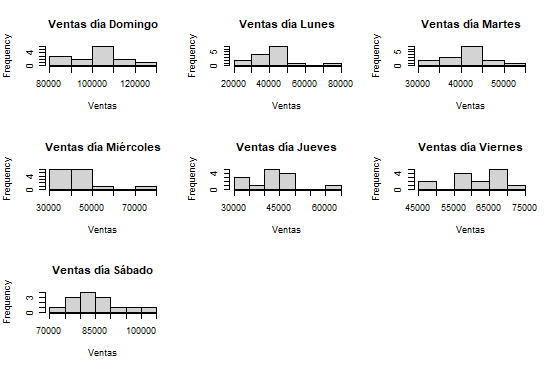
\includegraphics[width=0.8\textwidth,height=\textheight]{his_2.png}

}

\caption{Histogramas de las ventas por día después de la pandemia.}

\end{figure}%

El comportamiento periódico de las ventas, se observa en los boxplot de
las ventas por cada día de la semana.

\subsubsection{Boxplot de datos de ventas por días limpios después de la
pandemia}\label{boxplot-de-datos-de-ventas-por-duxedas-limpios-despuuxe9s-de-la-pandemia}

\begin{Shaded}
\begin{Highlighting}[]
\FunctionTok{summary}\NormalTok{(fil\_dat\_1\_after}\SpecialCharTok{$}\NormalTok{Ventas)}
\end{Highlighting}
\end{Shaded}

\begin{verbatim}
   Min. 1st Qu.  Median    Mean 3rd Qu.    Max. 
  80431   95346  103691  101919  107639  122397 
\end{verbatim}

\begin{Shaded}
\begin{Highlighting}[]
\FunctionTok{summary}\NormalTok{(fil\_dat\_2\_after}\SpecialCharTok{$}\NormalTok{Ventas)}
\end{Highlighting}
\end{Shaded}

\begin{verbatim}
   Min. 1st Qu.  Median    Mean 3rd Qu.    Max. 
  27106   33867   40804   42339   47566   77299 
\end{verbatim}

\begin{Shaded}
\begin{Highlighting}[]
\FunctionTok{summary}\NormalTok{(fil\_dat\_3\_after}\SpecialCharTok{$}\NormalTok{Ventas)}
\end{Highlighting}
\end{Shaded}

\begin{verbatim}
   Min. 1st Qu.  Median    Mean 3rd Qu.    Max. 
  30514   38860   41889   41752   44732   51733 
\end{verbatim}

\begin{Shaded}
\begin{Highlighting}[]
\FunctionTok{summary}\NormalTok{(fil\_dat\_4\_after}\SpecialCharTok{$}\NormalTok{Ventas)}
\end{Highlighting}
\end{Shaded}

\begin{verbatim}
   Min. 1st Qu.  Median    Mean 3rd Qu.    Max. 
  30335   34697   43071   43243   46480   70983 
\end{verbatim}

\begin{Shaded}
\begin{Highlighting}[]
\FunctionTok{summary}\NormalTok{(fil\_dat\_5\_after}\SpecialCharTok{$}\NormalTok{Ventas)}
\end{Highlighting}
\end{Shaded}

\begin{verbatim}
   Min. 1st Qu.  Median    Mean 3rd Qu.    Max. 
  31704   39901   43144   43010   47048   63104 
\end{verbatim}

\begin{Shaded}
\begin{Highlighting}[]
\FunctionTok{summary}\NormalTok{(fil\_dat\_6\_after}\SpecialCharTok{$}\NormalTok{Ventas)}
\end{Highlighting}
\end{Shaded}

\begin{verbatim}
   Min. 1st Qu.  Median    Mean 3rd Qu.    Max. 
  45908   56956   63361   61191   66915   70159 
\end{verbatim}

\begin{Shaded}
\begin{Highlighting}[]
\FunctionTok{summary}\NormalTok{(fil\_dat\_7\_after}\SpecialCharTok{$}\NormalTok{Ventas)}
\end{Highlighting}
\end{Shaded}

\begin{verbatim}
   Min. 1st Qu.  Median    Mean 3rd Qu.    Max. 
  73606   78646   84130   85684   89730  101467 
\end{verbatim}

El código que genera estos los boxplot en R es el siguiente:

\begin{Shaded}
\begin{Highlighting}[]
\CommentTok{\# muestra el gráfico de todos los boxplot de ventas por día antes de la pandemia }
\NormalTok{fig }\OtherTok{\textless{}{-}} \FunctionTok{plot\_ly}\NormalTok{(}\AttributeTok{y =}\NormalTok{fil\_dat\_1\_after}\SpecialCharTok{$}\NormalTok{Ventas, }\AttributeTok{name =} \StringTok{"Ventas día Domingo"}\NormalTok{,}
               \AttributeTok{boxpoints =} \StringTok{"all"}\NormalTok{,}\AttributeTok{type =} \StringTok{"box"}\NormalTok{)}

\NormalTok{fig }\OtherTok{\textless{}{-}}\NormalTok{ fig }\SpecialCharTok{\%\textgreater{}\%} \FunctionTok{add\_trace}\NormalTok{(}\AttributeTok{y =}\NormalTok{ fil\_dat\_2\_after}\SpecialCharTok{$}\NormalTok{Ventas,  }
                         \AttributeTok{name =} \StringTok{"Ventas día Lunes"}\NormalTok{, }\AttributeTok{boxpoints =} \StringTok{"all"}\NormalTok{)}
\NormalTok{fig }\OtherTok{\textless{}{-}}\NormalTok{ fig }\SpecialCharTok{\%\textgreater{}\%} \FunctionTok{add\_trace}\NormalTok{(}\AttributeTok{y =}\NormalTok{ fil\_dat\_3\_after}\SpecialCharTok{$}\NormalTok{Ventas,  }
                         \AttributeTok{name =} \StringTok{"Ventas día Martes"}\NormalTok{, }\AttributeTok{boxpoints =} \StringTok{"all"}\NormalTok{)}
\NormalTok{fig }\OtherTok{\textless{}{-}}\NormalTok{ fig }\SpecialCharTok{\%\textgreater{}\%} \FunctionTok{add\_trace}\NormalTok{(}\AttributeTok{y =}\NormalTok{ fil\_dat\_4\_after}\SpecialCharTok{$}\NormalTok{Ventas,  }
                         \AttributeTok{name =} \StringTok{"Ventas día Miércoles"}\NormalTok{, }\AttributeTok{boxpoints =} \StringTok{"all"}\NormalTok{)}
\NormalTok{fig }\OtherTok{\textless{}{-}}\NormalTok{ fig }\SpecialCharTok{\%\textgreater{}\%} \FunctionTok{add\_trace}\NormalTok{(}\AttributeTok{y =}\NormalTok{ fil\_dat\_5\_after}\SpecialCharTok{$}\NormalTok{Ventas,  }
                         \AttributeTok{name =} \StringTok{"Ventas día Jueves"}\NormalTok{, }\AttributeTok{boxpoints =} \StringTok{"all"}\NormalTok{)}
\NormalTok{fig }\OtherTok{\textless{}{-}}\NormalTok{ fig }\SpecialCharTok{\%\textgreater{}\%} \FunctionTok{add\_trace}\NormalTok{(}\AttributeTok{y =}\NormalTok{ fil\_dat\_6\_after}\SpecialCharTok{$}\NormalTok{Ventas,  }
                         \AttributeTok{name =} \StringTok{"Ventas día Viernes"}\NormalTok{, }\AttributeTok{boxpoints=}\StringTok{"all"}\NormalTok{)}
\NormalTok{fig }\OtherTok{\textless{}{-}}\NormalTok{ fig }\SpecialCharTok{\%\textgreater{}\%} \FunctionTok{add\_trace}\NormalTok{(}\AttributeTok{y =}\NormalTok{ fil\_dat\_7\_after}\SpecialCharTok{$}\NormalTok{Ventas,  }
                         \AttributeTok{name =} \StringTok{"Ventas día Sábado"}\NormalTok{, }\AttributeTok{boxpoints =} \StringTok{"all"}\NormalTok{)}
\NormalTok{fig}
\end{Highlighting}
\end{Shaded}

\begin{figure}[H]

{\centering 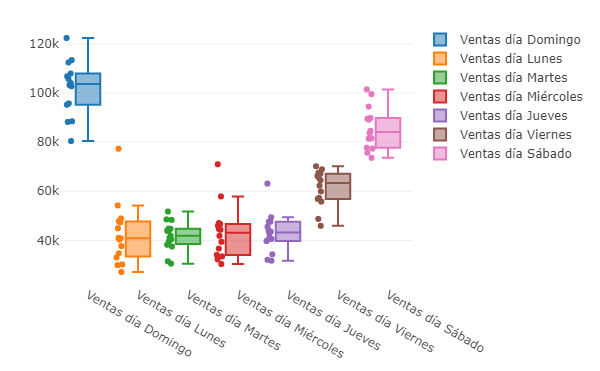
\includegraphics{fig-box2pdf.png}

}

\caption{Boxplot de las ventas por día después de la pandemia.}

\end{figure}%

\section{Identificación de distribuciones de probabilidad de las ventas
por
día}\label{identificaciuxf3n-de-distribuciones-de-probabilidad-de-las-ventas-por-duxeda}

Con el fin de adaptar el modelo de Cramér Lundberg es necesario ajustar
distribuciones de probabilidad de las ventas para cada día de la semana.
Haciendo uso del test de Jarque Bera que ayuda a identificar cuales días
siguen una distribución normal y el test de Kolmogorov de Smirnov.

El siguiente código aplica los diferentes test de normalidad para las
ventas por día antes de la pandemia:(Citar Jarque Bera)

\begin{Shaded}
\begin{Highlighting}[]
\CommentTok{\#Calcularemos los test correspondientes a los filtros}
\CommentTok{\#de ventas por día:}

\CommentTok{\#JARQUE BERA}
\FunctionTok{jarque.bera.test}\NormalTok{(fil\_dat\_1\_before}\SpecialCharTok{$}\NormalTok{Ventas)}
\end{Highlighting}
\end{Shaded}

\begin{verbatim}

    Jarque Bera Test

data:  fil_dat_1_before$Ventas
X-squared = 4.3177, df = 2, p-value = 0.1155
\end{verbatim}

\begin{Shaded}
\begin{Highlighting}[]
\CommentTok{\#El valor p no es menor que α = .05, }
\CommentTok{\#entonces hay evidencia suficiente para decir }
\CommentTok{\#por lo tanto los datos se distribuyen normalmente}
\CommentTok{\#Se ajustara una distribuciión con el comando siguiente:}

\FunctionTok{fitdistr}\NormalTok{(fil\_dat\_1\_before}\SpecialCharTok{$}\NormalTok{Ventas, }\StringTok{"normal"}\NormalTok{)}
\end{Highlighting}
\end{Shaded}

\begin{verbatim}
      mean          sd    
  139929.468    24521.524 
 (  2675.518) (  1891.877)
\end{verbatim}

\begin{Shaded}
\begin{Highlighting}[]
\CommentTok{\#JARQUE BERA}
\FunctionTok{jarque.bera.test}\NormalTok{(fil\_dat\_2\_before}\SpecialCharTok{$}\NormalTok{Ventas)}
\end{Highlighting}
\end{Shaded}

\begin{verbatim}

    Jarque Bera Test

data:  fil_dat_2_before$Ventas
X-squared = 2.7606, df = 2, p-value = 0.2515
\end{verbatim}

\begin{Shaded}
\begin{Highlighting}[]
\CommentTok{\#El valor p no es menor que α = .05, }
\CommentTok{\#entonces hay evidencia suficiente para decir }
\CommentTok{\#por lo tanto los datos se distribuyen normalmente}
\CommentTok{\#Se ajustara una distribuciión con el comando siguiente:}
\CommentTok{\#ajustamos una distribución (normal)}
\FunctionTok{fitdistr}\NormalTok{(fil\_dat\_2\_before}\SpecialCharTok{$}\NormalTok{Ventas, }\StringTok{"normal"}\NormalTok{)}
\end{Highlighting}
\end{Shaded}

\begin{verbatim}
     mean         sd    
  48125.734   17150.338 
 ( 1917.466) ( 1355.853)
\end{verbatim}

\begin{Shaded}
\begin{Highlighting}[]
\CommentTok{\#JARQUE BERA}
\FunctionTok{jarque.bera.test}\NormalTok{(fil\_dat\_3\_before}\SpecialCharTok{$}\NormalTok{Ventas)}
\end{Highlighting}
\end{Shaded}

\begin{verbatim}

    Jarque Bera Test

data:  fil_dat_3_before$Ventas
X-squared = 4.6048, df = 2, p-value = 0.1
\end{verbatim}

\begin{Shaded}
\begin{Highlighting}[]
\CommentTok{\#El valor p no es menor que α = .05, }
\CommentTok{\#entonces hay evidencia suficiente para decir }
\CommentTok{\#por lo tanto los datos se distribuyen normalmente}
\CommentTok{\#Se ajustara una distribuciión con el comando siguiente:}
\CommentTok{\#ajustamos una distribución (normal)}
\FunctionTok{fitdistr}\NormalTok{(fil\_dat\_3\_before}\SpecialCharTok{$}\NormalTok{Ventas, }\StringTok{"normal"}\NormalTok{)}
\end{Highlighting}
\end{Shaded}

\begin{verbatim}
     mean         sd    
  44509.755   14312.338 
 ( 1590.260) ( 1124.483)
\end{verbatim}

\begin{Shaded}
\begin{Highlighting}[]
\CommentTok{\#JARQUE BERA}
\FunctionTok{jarque.bera.test}\NormalTok{(fil\_dat\_4\_before}\SpecialCharTok{$}\NormalTok{Ventas)}
\end{Highlighting}
\end{Shaded}

\begin{verbatim}

    Jarque Bera Test

data:  fil_dat_4_before$Ventas
X-squared = 3.3204, df = 2, p-value = 0.1901
\end{verbatim}

\begin{Shaded}
\begin{Highlighting}[]
\CommentTok{\#El valor p no es menor que α = .05, }
\CommentTok{\#entonces hay evidencia suficiente para decir }
\CommentTok{\#por lo tanto los datos se distribuyen normalmente}
\CommentTok{\#Se ajustara una distribuciión con el comando siguiente:}
\CommentTok{\#ajustamos una distribución (normal)}
\FunctionTok{fitdistr}\NormalTok{(fil\_dat\_4\_before}\SpecialCharTok{$}\NormalTok{Ventas, }\StringTok{"normal"}\NormalTok{)}
\end{Highlighting}
\end{Shaded}

\begin{verbatim}
     mean         sd    
  46904.516   16238.151 
 ( 1815.480) ( 1283.739)
\end{verbatim}

\begin{Shaded}
\begin{Highlighting}[]
\CommentTok{\#JARQUE BERA}
\FunctionTok{jarque.bera.test}\NormalTok{(fil\_dat\_5\_before}\SpecialCharTok{$}\NormalTok{Ventas)}
\end{Highlighting}
\end{Shaded}

\begin{verbatim}

    Jarque Bera Test

data:  fil_dat_5_before$Ventas
X-squared = 4.553, df = 2, p-value = 0.1026
\end{verbatim}

\begin{Shaded}
\begin{Highlighting}[]
\CommentTok{\#El valor p no es menor que α = .05, }
\CommentTok{\#entonces hay evidencia suficiente para decir }
\CommentTok{\#por lo tanto los datos se distribuyen normalmente}
\CommentTok{\#Se ajustara una distribuciión con el comando siguiente:}
\CommentTok{\#ajustamos una distribución (normal)}
\FunctionTok{fitdistr}\NormalTok{(fil\_dat\_5\_before}\SpecialCharTok{$}\NormalTok{Ventas, }\StringTok{"normal"}\NormalTok{)}
\end{Highlighting}
\end{Shaded}

\begin{verbatim}
     mean         sd    
  52786.734   18403.175 
 ( 2032.291) ( 1437.047)
\end{verbatim}

\begin{Shaded}
\begin{Highlighting}[]
\CommentTok{\#JARQUE BERA}
\FunctionTok{jarque.bera.test}\NormalTok{(fil\_dat\_6\_before}\SpecialCharTok{$}\NormalTok{Ventas)}
\end{Highlighting}
\end{Shaded}

\begin{verbatim}

    Jarque Bera Test

data:  fil_dat_6_before$Ventas
X-squared = 2.5406, df = 2, p-value = 0.2808
\end{verbatim}

\begin{Shaded}
\begin{Highlighting}[]
\CommentTok{\#El valor p no es menor que α = .05, }
\CommentTok{\#entonces hay evidencia suficiente para decir }
\CommentTok{\#por lo tanto los datos se distribuyen normalmente}
\CommentTok{\#Se ajustara una distribuciión con el comando siguiente:}
\CommentTok{\#ajustamos una distribución (normal)}
\FunctionTok{fitdistr}\NormalTok{(fil\_dat\_6\_before}\SpecialCharTok{$}\NormalTok{Ventas, }\StringTok{"normal"}\NormalTok{)}
\end{Highlighting}
\end{Shaded}

\begin{verbatim}
     mean         sd    
  81601.876   23756.037 
 ( 2591.996) ( 1832.818)
\end{verbatim}

Para el caso del día sábado, denotado como séptimo día, no se obtuvo una
distribución normal por lo que se utilizo la paqueteria de R
fitdistrplus para probar el ajuste de otras distribuciones clásicas de
probabilidad. Las distribuciones probadas se presentan en el código
siguiente:

\begin{Shaded}
\begin{Highlighting}[]
\FunctionTok{fitdistr}\NormalTok{(fil\_dat\_7\_before}\SpecialCharTok{$}\NormalTok{Ventas, }\StringTok{"weibull"}\NormalTok{)}
\end{Highlighting}
\end{Shaded}

\begin{verbatim}
      shape          scale    
  3.646021e+00   1.335448e+05 
 (2.784858e-01) (4.365588e+03)
\end{verbatim}

\begin{Shaded}
\begin{Highlighting}[]
\FunctionTok{fitdistr}\NormalTok{(fil\_dat\_7\_before}\SpecialCharTok{$}\NormalTok{Ventas, }\StringTok{"exponential"}\NormalTok{)}
\end{Highlighting}
\end{Shaded}

\begin{verbatim}
       rate    
  8.379989e-06 
 (8.882771e-07)
\end{verbatim}

\begin{Shaded}
\begin{Highlighting}[]
\FunctionTok{fitdistr}\NormalTok{(fil\_dat\_7\_before}\SpecialCharTok{$}\NormalTok{Ventas, }\StringTok{"lognormal"}\NormalTok{)}
\end{Highlighting}
\end{Shaded}

\begin{verbatim}
     meanlog        sdlog   
  11.64220349    0.33374967 
 ( 0.03537739) ( 0.02501560)
\end{verbatim}

De lo anterior podemos decir que el mejor ajuste se obtuvo al usar la
distribución Weibull.

\subsection{Prueba de la distribución
Weibull:}\label{prueba-de-la-distribuciuxf3n-weibull}

Una vez ajustada la distribución Weibull, se prueban sus parametros con
la aplicación del test de Kolmogorov de Smirnov. El siguiente código
implementa ambos procedimientos:

\begin{Shaded}
\begin{Highlighting}[]
\CommentTok{\#Calcularemos los test correspondientes a los filtros de de ventas por día:}
\CommentTok{\#JARQUE BERA}
\FunctionTok{jarque.bera.test}\NormalTok{(fil\_dat\_7\_before}\SpecialCharTok{$}\NormalTok{Ventas)}
\end{Highlighting}
\end{Shaded}

\begin{verbatim}

    Jarque Bera Test

data:  fil_dat_7_before$Ventas
X-squared = 12.707, df = 2, p-value = 0.001741
\end{verbatim}

\begin{Shaded}
\begin{Highlighting}[]
\CommentTok{\#Fitting de de una distri bución weibull}
\CommentTok{\#fil\_dat\_7\_before$Ventas}
\NormalTok{fit.weibull }\OtherTok{\textless{}{-}} \FunctionTok{fitdist}\NormalTok{(fil\_dat\_7\_before}\SpecialCharTok{$}\NormalTok{Ventas, }\StringTok{"weibull"}\NormalTok{)}
\NormalTok{fit.weibull}
\end{Highlighting}
\end{Shaded}

\begin{verbatim}
Fitting of the distribution ' weibull ' by maximum likelihood 
Parameters:
          estimate   Std. Error
shape 4.784508e+00    0.3789532
scale 1.295070e+05 3155.3275585
\end{verbatim}

\begin{Shaded}
\begin{Highlighting}[]
\NormalTok{vector\_ventas7\_ordenados }\OtherTok{\textless{}{-}}\NormalTok{ fil\_dat\_7\_before}\SpecialCharTok{$}\NormalTok{Ventas[}\FunctionTok{order}\NormalTok{(fil\_dat\_7\_before}\SpecialCharTok{$}\NormalTok{Ventas)]}
\NormalTok{n }\OtherTok{=} \DecValTok{83}
\NormalTok{F\_x }\OtherTok{=} \FunctionTok{numeric}\NormalTok{(n)}
\ControlFlowTok{for}\NormalTok{(i }\ControlFlowTok{in} \DecValTok{1}\SpecialCharTok{:}\NormalTok{n)\{}
\NormalTok{  F\_x[i] }\OtherTok{\textless{}{-}}\NormalTok{ (i}\SpecialCharTok{/}\NormalTok{ n)}
\NormalTok{\}}
\CommentTok{\#F\_x}
\NormalTok{f\_gorro\_x }\OtherTok{\textless{}{-}}  \FunctionTok{pweibull}\NormalTok{(vector\_ventas7\_ordenados,}
                       \AttributeTok{shape =} \FloatTok{4.784508e+00}\NormalTok{, }\AttributeTok{scale =}\FloatTok{1.295070e+05}\NormalTok{, }
                       \AttributeTok{lower.tail =} \ConstantTok{TRUE}\NormalTok{, }\AttributeTok{log.p =} \ConstantTok{FALSE}\NormalTok{)}
\NormalTok{ks }\OtherTok{\textless{}{-}} \FunctionTok{abs}\NormalTok{(F\_x }\SpecialCharTok{{-}}\NormalTok{ f\_gorro\_x)}
\end{Highlighting}
\end{Shaded}

\subsubsection{Representación gráfica al aplicar el test de Kolmogorov
de
Smirnov}\label{representaciuxf3n-gruxe1fica-al-aplicar-el-test-de-kolmogorov-de-smirnov}

\begin{verbatim}
[1] 0.1936014
\end{verbatim}

\begin{verbatim}
[1] 0.1492794
\end{verbatim}

\begin{Shaded}
\begin{Highlighting}[]
\NormalTok{x }\OtherTok{\textless{}{-}} \DecValTok{1}\SpecialCharTok{:}\DecValTok{83} 
\NormalTok{g1 }\OtherTok{\textless{}{-}} \FunctionTok{plot}\NormalTok{(}\DecValTok{1}\SpecialCharTok{:}\DecValTok{83}\NormalTok{, F\_x) }
\end{Highlighting}
\end{Shaded}

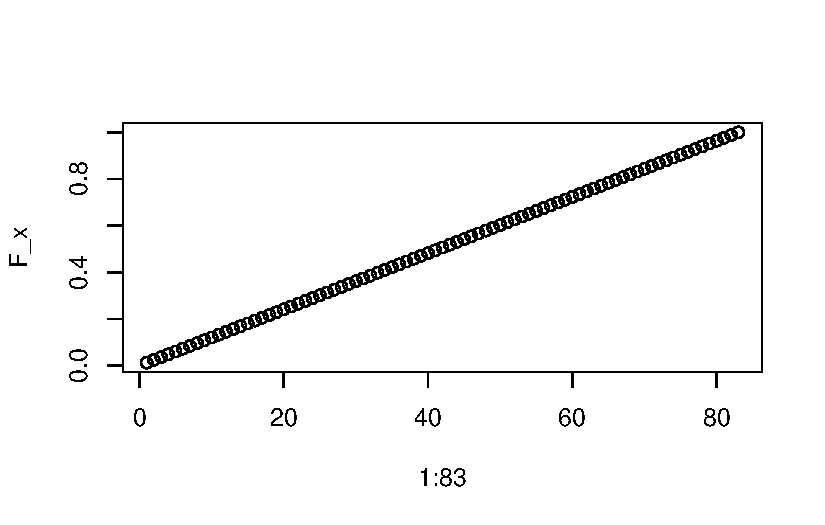
\includegraphics{Estudio_caso_files/figure-pdf/unnamed-chunk-27-1.pdf}

\begin{Shaded}
\begin{Highlighting}[]
\NormalTok{g2 }\OtherTok{\textless{}{-}} \FunctionTok{plot}\NormalTok{(}\DecValTok{1}\SpecialCharTok{:}\DecValTok{83}\NormalTok{, f\_gorro\_x) }
\end{Highlighting}
\end{Shaded}

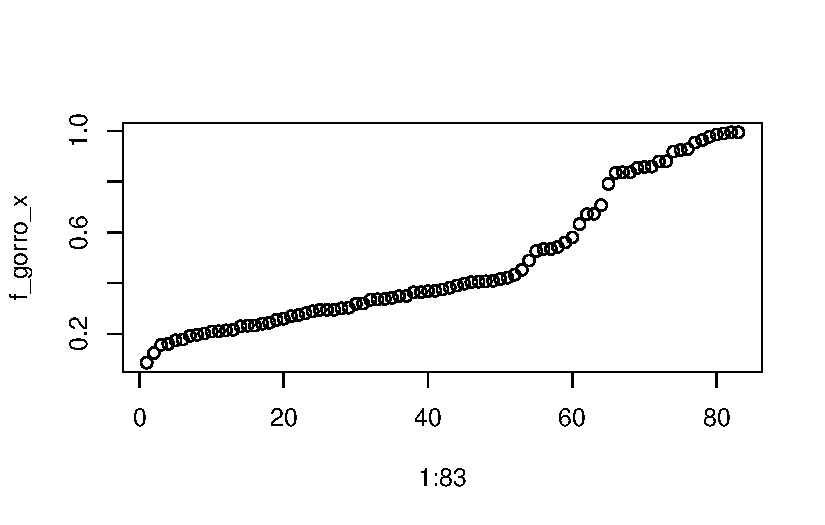
\includegraphics{Estudio_caso_files/figure-pdf/unnamed-chunk-27-2.pdf}

\begin{Shaded}
\begin{Highlighting}[]
\FunctionTok{plot}\NormalTok{(x, F\_x, }\AttributeTok{col=}\StringTok{\textquotesingle{}red\textquotesingle{}}\NormalTok{, }\AttributeTok{xlab=}\StringTok{\textquotesingle{}x\textquotesingle{}}\NormalTok{, }\AttributeTok{ylab=}\StringTok{\textquotesingle{}y\textquotesingle{}}\NormalTok{)}

\CommentTok{\#add second line to plot }
\FunctionTok{points}\NormalTok{(x, f\_gorro\_x, }\AttributeTok{col=}\StringTok{\textquotesingle{}blue\textquotesingle{}}\NormalTok{)}
\end{Highlighting}
\end{Shaded}

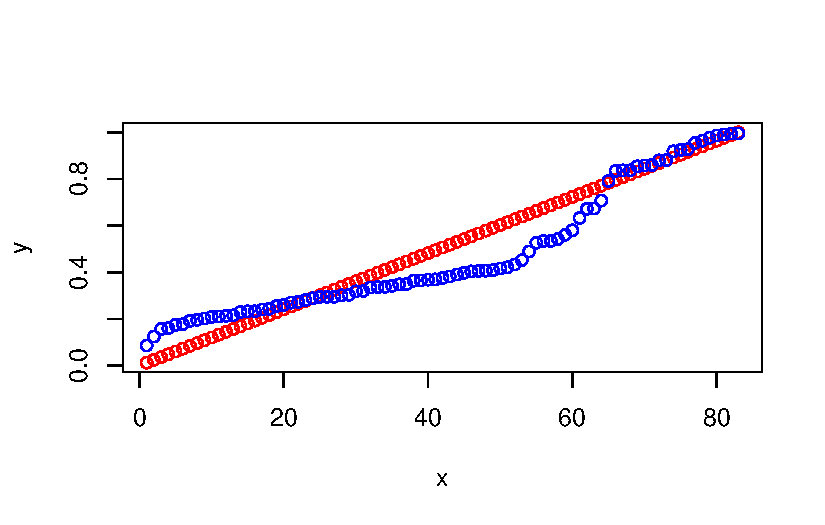
\includegraphics{Estudio_caso_files/figure-pdf/unnamed-chunk-27-3.pdf}

Para el periodo despues de pandemia se repite la misma metodología.
Aplicamos el test de Jarque Bera a los datos para cada día de la semana
después de pandemia.

\begin{verbatim}

    Jarque Bera Test

data:  fil_dat_1_after$Ventas
X-squared = 0.24366, df = 2, p-value = 0.8853
\end{verbatim}

\begin{verbatim}
      mean          sd    
  101919.050    10877.075 
 (  2907.021) (  2055.574)
\end{verbatim}

\begin{verbatim}

    Jarque Bera Test

data:  fil_dat_2_after$Ventas
X-squared = 0.65149, df = 2, p-value = 0.722
\end{verbatim}

\begin{verbatim}
     mean         sd    
  39841.721    7873.446 
 ( 2104.267) ( 1487.941)
\end{verbatim}

\begin{verbatim}

    Jarque Bera Test

data:  fil_dat_3_after$Ventas
X-squared = 0.39157, df = 2, p-value = 0.8222
\end{verbatim}

\begin{verbatim}
     mean         sd    
  41751.747    5687.030 
 ( 1468.385) ( 1038.305)
\end{verbatim}

\begin{verbatim}

    Jarque Bera Test

data:  fil_dat_4_after$Ventas
X-squared = 3.8727, df = 2, p-value = 0.1442
\end{verbatim}

\begin{verbatim}
     mean         sd    
  43243.143   10517.841 
 ( 2811.011) ( 1987.685)
\end{verbatim}

\begin{verbatim}

    Jarque Bera Test

data:  fil_dat_5_after$Ventas
X-squared = 2.0444, df = 2, p-value = 0.3598
\end{verbatim}

\begin{verbatim}
     mean         sd    
  43010.307    7741.889 
 ( 2069.107) ( 1463.080)
\end{verbatim}

\begin{verbatim}

    Jarque Bera Test

data:  fil_dat_6_after$Ventas
X-squared = 1.4585, df = 2, p-value = 0.4823
\end{verbatim}

\begin{verbatim}
     mean         sd    
  61191.300    7202.989 
 ( 1925.080) ( 1361.237)
\end{verbatim}

\begin{verbatim}

    Jarque Bera Test

data:  fil_dat_7_after$Ventas
X-squared = 0.85511, df = 2, p-value = 0.6521
\end{verbatim}

\begin{verbatim}
     mean         sd    
  85684.058    8371.359 
 ( 2237.340) ( 1582.038)
\end{verbatim}

\begin{Shaded}
\begin{Highlighting}[]
\CommentTok{\#\_\_\_\_\_\_\_Después de la pandemia\_\_\_\_\_\_\_\_\_\_\_\_\_\_\_\_\_\_\_\_\_\_\_\_\_\_\_\_\_\_\_\_\_\_\_\_}
\CommentTok{\#El valor p no es menor que α = .05, }
\CommentTok{\#entonces hay evidencia suficiente para decir }
\CommentTok{\#que la muestra  proviene de una población con distribución normal.}
\CommentTok{\#JARQUE BERA}
\FunctionTok{jarque.bera.test}\NormalTok{(fil\_dat\_1\_after}\SpecialCharTok{$}\NormalTok{Ventas)}
\end{Highlighting}
\end{Shaded}

\begin{verbatim}

    Jarque Bera Test

data:  fil_dat_1_after$Ventas
X-squared = 0.24366, df = 2, p-value = 0.8853
\end{verbatim}

\begin{Shaded}
\begin{Highlighting}[]
\FunctionTok{fitdistr}\NormalTok{(fil\_dat\_1\_after}\SpecialCharTok{$}\NormalTok{Ventas, }\StringTok{"normal"}\NormalTok{)}
\end{Highlighting}
\end{Shaded}

\begin{verbatim}
      mean          sd    
  101919.050    10877.075 
 (  2907.021) (  2055.574)
\end{verbatim}

\begin{Shaded}
\begin{Highlighting}[]
\CommentTok{\#\_\_\_\_\_\_\_\_\_\_\_\_\_\_\_\_\_\_\_\_\_\_\_\_\_\_\_\_\_\_\_\_\_\_\_\_\_\_\_\_\_\_\_\_\_\_\_\_\_\_\_\_\_\_\_\_\_\_\_\_\_\_\_\_}
\CommentTok{\#Calcularemos los test correspondientes }
\CommentTok{\#a los filtros de de ventas por día:}
\CommentTok{\#El valor p no es menor que α = .05, }
\CommentTok{\#entonces hay evidencia suficiente para decir }
\CommentTok{\#que la muestra proviene de una población con distribución normal.}
\CommentTok{\#JARQUE BERA}
\FunctionTok{jarque.bera.test}\NormalTok{(fil\_dat\_2\_after}\SpecialCharTok{$}\NormalTok{Ventas)}
\end{Highlighting}
\end{Shaded}

\begin{verbatim}

    Jarque Bera Test

data:  fil_dat_2_after$Ventas
X-squared = 0.65149, df = 2, p-value = 0.722
\end{verbatim}

\begin{Shaded}
\begin{Highlighting}[]
\FunctionTok{fitdistr}\NormalTok{(fil\_dat\_2\_after}\SpecialCharTok{$}\NormalTok{Ventas, }\StringTok{"normal"}\NormalTok{)}
\end{Highlighting}
\end{Shaded}

\begin{verbatim}
     mean         sd    
  39841.721    7873.446 
 ( 2104.267) ( 1487.941)
\end{verbatim}

\begin{Shaded}
\begin{Highlighting}[]
\CommentTok{\#\_\_\_\_\_\_\_\_\_\_\_\_\_\_\_\_\_\_\_\_\_\_\_\_\_\_\_\_\_\_\_\_\_\_\_\_\_\_\_\_\_\_\_\_\_\_\_\_\_\_\_\_\_\_\_\_\_\_\_\_\_\_\_\_}
\CommentTok{\#Calcularemos los test correspondientes }
\CommentTok{\# a los filtros de de ventas por día:}
\CommentTok{\#El valor p no es menor que α = .05, }
\CommentTok{\#entonces hay evidencia suficiente para decir }
\CommentTok{\#que la muestra proviene de una población con distribución normal.}
\CommentTok{\#JARQUE BERA}
\FunctionTok{jarque.bera.test}\NormalTok{(fil\_dat\_3\_after}\SpecialCharTok{$}\NormalTok{Ventas)}
\end{Highlighting}
\end{Shaded}

\begin{verbatim}

    Jarque Bera Test

data:  fil_dat_3_after$Ventas
X-squared = 0.39157, df = 2, p-value = 0.8222
\end{verbatim}

\begin{Shaded}
\begin{Highlighting}[]
\FunctionTok{fitdistr}\NormalTok{(fil\_dat\_3\_after}\SpecialCharTok{$}\NormalTok{Ventas, }\StringTok{"normal"}\NormalTok{)}
\end{Highlighting}
\end{Shaded}

\begin{verbatim}
     mean         sd    
  41751.747    5687.030 
 ( 1468.385) ( 1038.305)
\end{verbatim}

\begin{Shaded}
\begin{Highlighting}[]
\CommentTok{\#\_\_\_\_\_\_\_\_\_\_\_\_\_\_\_\_\_\_\_\_\_\_\_\_\_\_\_\_\_\_\_\_\_\_\_\_\_\_\_\_\_\_\_\_\_\_\_\_\_\_\_\_\_\_\_\_\_\_\_\_\_\_\_\_}
\CommentTok{\#Calcularemos los test correspondientes }
\CommentTok{\# a los filtros de de ventas por día:}
\CommentTok{\#El valor p no es menor que α = .05, }
\CommentTok{\#entonces hay evidencia suficiente para decir }
\CommentTok{\#que la muestra proviene de una población con distribución normal.}
\CommentTok{\#JARQUE BERA}
\FunctionTok{jarque.bera.test}\NormalTok{(fil\_dat\_4\_after}\SpecialCharTok{$}\NormalTok{Ventas)}
\end{Highlighting}
\end{Shaded}

\begin{verbatim}

    Jarque Bera Test

data:  fil_dat_4_after$Ventas
X-squared = 3.8727, df = 2, p-value = 0.1442
\end{verbatim}

\begin{Shaded}
\begin{Highlighting}[]
\FunctionTok{fitdistr}\NormalTok{(fil\_dat\_4\_after}\SpecialCharTok{$}\NormalTok{Ventas, }\StringTok{"normal"}\NormalTok{)}
\end{Highlighting}
\end{Shaded}

\begin{verbatim}
     mean         sd    
  43243.143   10517.841 
 ( 2811.011) ( 1987.685)
\end{verbatim}

\begin{Shaded}
\begin{Highlighting}[]
\CommentTok{\#\_\_\_\_\_\_\_\_\_\_\_\_\_\_\_\_\_\_\_\_\_\_\_\_\_\_\_\_\_\_\_\_\_\_\_\_\_\_\_\_\_\_\_\_\_\_\_\_\_\_\_\_\_\_\_\_\_\_\_\_\_\_\_\_}
\CommentTok{\#Calcularemos los test correspondientes }
\CommentTok{\# a los filtros de de ventas por día:}
\CommentTok{\#El valor p no es menor que α = .05, }
\CommentTok{\#entonces hay evidencia suficiente para decir }
\CommentTok{\#que la muestra proviene de una población con distribución normal.}
\CommentTok{\#JARQUE BERA}
\FunctionTok{jarque.bera.test}\NormalTok{(fil\_dat\_5\_after}\SpecialCharTok{$}\NormalTok{Ventas)}
\end{Highlighting}
\end{Shaded}

\begin{verbatim}

    Jarque Bera Test

data:  fil_dat_5_after$Ventas
X-squared = 2.0444, df = 2, p-value = 0.3598
\end{verbatim}

\begin{Shaded}
\begin{Highlighting}[]
\FunctionTok{fitdistr}\NormalTok{(fil\_dat\_5\_after}\SpecialCharTok{$}\NormalTok{Ventas, }\StringTok{"normal"}\NormalTok{)}
\end{Highlighting}
\end{Shaded}

\begin{verbatim}
     mean         sd    
  43010.307    7741.889 
 ( 2069.107) ( 1463.080)
\end{verbatim}

\begin{Shaded}
\begin{Highlighting}[]
\CommentTok{\#\_\_\_\_\_\_\_\_\_\_\_\_\_\_\_\_\_\_\_\_\_\_\_\_\_\_\_\_\_\_\_\_\_\_\_\_\_\_\_\_\_\_\_\_\_\_\_\_\_\_\_\_\_\_\_\_\_\_\_\_\_\_\_\_}
\CommentTok{\#Calcularemos los test correspondientes }
\CommentTok{\# a los filtros de de ventas por día:}
\CommentTok{\# El valor p no es menor que α = .05, }
\CommentTok{\#entonces hay evidencia suficiente para decir }
\CommentTok{\#que la muestra proviene de una población con distribución normal.}
\CommentTok{\#JARQUE BERA}
\FunctionTok{jarque.bera.test}\NormalTok{(fil\_dat\_6\_after}\SpecialCharTok{$}\NormalTok{Ventas)}
\end{Highlighting}
\end{Shaded}

\begin{verbatim}

    Jarque Bera Test

data:  fil_dat_6_after$Ventas
X-squared = 1.4585, df = 2, p-value = 0.4823
\end{verbatim}

\begin{Shaded}
\begin{Highlighting}[]
\FunctionTok{fitdistr}\NormalTok{(fil\_dat\_6\_after}\SpecialCharTok{$}\NormalTok{Ventas, }\StringTok{"normal"}\NormalTok{)}
\end{Highlighting}
\end{Shaded}

\begin{verbatim}
     mean         sd    
  61191.300    7202.989 
 ( 1925.080) ( 1361.237)
\end{verbatim}

\begin{Shaded}
\begin{Highlighting}[]
\CommentTok{\#\_\_\_\_\_\_\_\_\_\_\_\_\_\_\_\_\_\_\_\_\_\_\_\_\_\_\_\_\_\_\_\_\_\_\_\_\_\_\_\_\_\_\_\_\_\_\_\_\_\_\_\_\_\_\_\_\_\_\_\_\_\_\_\_}
\CommentTok{\#Calcularemos los test correspondientes }
\CommentTok{\# a los filtros de de ventas por día:}
\CommentTok{\#El valor p no es menor que α = .05, }
\CommentTok{\#entonces hay evidencia suficiente para decir }
\CommentTok{\#que la muestra proviene de una población con distribución normal.}
\FunctionTok{jarque.bera.test}\NormalTok{(fil\_dat\_7\_after}\SpecialCharTok{$}\NormalTok{Ventas)}
\end{Highlighting}
\end{Shaded}

\begin{verbatim}

    Jarque Bera Test

data:  fil_dat_7_after$Ventas
X-squared = 0.85511, df = 2, p-value = 0.6521
\end{verbatim}

\begin{Shaded}
\begin{Highlighting}[]
\CommentTok{\#Se ajustara una distribución con el comando siguiente:}
\FunctionTok{fitdistr}\NormalTok{(fil\_dat\_7\_after}\SpecialCharTok{$}\NormalTok{Ventas, }\StringTok{"normal"}\NormalTok{)}
\end{Highlighting}
\end{Shaded}

\begin{verbatim}
     mean         sd    
  85684.058    8371.359 
 ( 2237.340) ( 1582.038)
\end{verbatim}

Con las distribuciones identificadas de las ventas por día en los dos
periodos, ahora es posible simular las variables aleatorias de las
ventas de cada día de la semana y por lo tanto simular las ganancias de
toda la semana.

\section{Modelo Modificado de Cramér-Lundberg para identificar la
probabilidad de las ganancias insuficientes en una empresa de comida
rápida}\label{modelo-modificado-de-cramuxe9r-lundberg-para-identificar-la-probabilidad-de-las-ganancias-insuficientes-en-una-empresa-de-comida-ruxe1pida}

Como ya se vio en la sección (Capítulo~\ref{sec-modelo_C_L}) El Modelo
de Cramér-Lundberg (MCL) es una herramienta utilizada en el campo de la
gestión de riesgos y las finanzas para evaluar la probabilidad de
incumplimiento o pérdidas insuficientes en una empresa. Aunque no es
específicamente diseñado para analizar la variación de las ganancias de
una empresa, en particular una empresa de comida rápida, puede adaptarse
para evaluar la probabilidad de ganancias insuficientes en este tipo de
negocio, que puede llevar a la decisión de cierre de las actividades de
la empresa.

Para ello la ecuación general del modelo modificado que representa la
evolución de las ganancias en el tiempo hasta la semana \(t\), denotada
por \(G\) queda definida como:
\begin{equation}\phantomsection\label{eq-4.1pdf}{G(t) = u -ct + V(t), \ \ t = 1, 2, 3, ...}\end{equation}

la cual se estudiara en los dos periodo de tiempo (pre-pandemia,
pos-pandemia).

\begin{itemize}
\item
  \(V(t)\): son los ingresos de las ganancias por día para cada semana
\item
  \(c\) : Son los costos de las obligaciones financieras del
  inversionista, como prestamos, pagos por adquisición de la franquicia,
  compras de equipos inmobiliarios, pagos de empleados, etc.
\item
  \(u \geq 0\) : Es el capital inicial con el cual inicia la empresa a
  trabajar.
\end{itemize}

\subsection{Caso pre-pandemia}\label{caso-pre-pandemia}

Para la implementación del modelo modificado Cramér-Lundberg con los
datos antes de la pandemia se hizo la simulación de las variables
aleatorias mediante las distribuciones de las ventas por día tomado como
las ganancias acumuladas, y se estimó los parámetros de \(u\) y \(c\),
por lo que el modelo es determinista y se incrementa por semana.

\subsubsection{Modelo de Cramér-Lundberg simulado en R con datos reales
de las ventas por día de la
empresa.}\label{modelo-de-cramuxe9r-lundberg-simulado-en-r-con-datos-reales-de-las-ventas-por-duxeda-de-la-empresa.}

En la (Figura~\ref{fig-fig-trayectoriapdf}) se muestra la trayectoria
del modelo bajo los supuestos del modelo modificado, el proceso comienza
con \(t = 90\), que son las \(90\) semanas de de las ventas registradas
por día antes del cierre pandemico, con un capital inicial de
\(u= 1759629\), una tasa de \(c= 0.29\), los montos de las ganancias
tienen distribución normal y weibull.

El código que genera la trayectoria es el siguiente:

\begin{Shaded}
\begin{Highlighting}[]
\CommentTok{\#Simulación Modelo Clásico de Cramér{-}Lundberg }
\CommentTok{\#para tres meses: Antes de la pandemia}
\CommentTok{\#Con los datos reales de la empresa}
\FunctionTok{library}\NormalTok{(dplyr)}\CommentTok{\#librería para poder renombrar las cabeceras }
\CommentTok{\# de los dataframes}
\CommentTok{\#Parámetros}
\FunctionTok{set.seed}\NormalTok{(}\DecValTok{13}\NormalTok{) }\CommentTok{\#semilla fija}
\NormalTok{u }\OtherTok{=} \DecValTok{1759629} \CommentTok{\#surplus(capital inicial de salvamento)}
\CommentTok{\#Es un estimado a partir de la media de las ganancias por semana, }
\CommentTok{\#multiplicado por 10/3, }
\CommentTok{\#siendo una proporción para evitar la ruina}
\CommentTok{\# u (sum(medias))*(10/3)}
\NormalTok{c }\OtherTok{=}\FloatTok{0.29}\SpecialCharTok{*}\NormalTok{u }\CommentTok{\#prima de pago cada timepo t. c=0.5*u}
\NormalTok{t\_final }\OtherTok{=} \DecValTok{90}
\CommentTok{\# S(t) = \textbackslash{}sum\_\{i=1\}\^{}\{N(t)\}X\_i}
\CommentTok{\#donde N(t)\textasciitilde{} Poisson (lambda*t)}
\CommentTok{\# X\_i \textasciitilde{} exponencial (lambda\_Xi)}
\CommentTok{\#CL = REPRESENTA EL MODELO DE CRAMER LUNDBERG}
\CommentTok{\#Simulación de trayectoria de CL\_t, cuando t \textless{} t\_final.}
\NormalTok{trayectoria\_CLt }\OtherTok{\textless{}{-}} \ControlFlowTok{function}\NormalTok{(u, c, t\_final)}
\NormalTok{\{}
\NormalTok{  tiempo }\OtherTok{\textless{}{-}} \FunctionTok{c}\NormalTok{(}\DecValTok{0}\NormalTok{)}
\NormalTok{  Cramer\_trayectoria }\OtherTok{\textless{}{-}} \FunctionTok{c}\NormalTok{(u)}
  \ControlFlowTok{while}\NormalTok{(tiempo[}\FunctionTok{length}\NormalTok{(tiempo)] }\SpecialCharTok{\textless{}}\NormalTok{ t\_final)}
\NormalTok{  \{}
\NormalTok{    tiempo\_llegada }\OtherTok{\textless{}{-}}\NormalTok{ (}\DecValTok{1}\NormalTok{)}
\NormalTok{  Y\_i }\OtherTok{\textless{}{-}}\NormalTok{  (}\FunctionTok{rnorm}\NormalTok{(}\DecValTok{1}\NormalTok{, }\AttributeTok{mean =} \FloatTok{139929.468}\NormalTok{, }\AttributeTok{sd =} \FloatTok{24521.524}\NormalTok{ )  }\SpecialCharTok{+} 
            \FunctionTok{rnorm}\NormalTok{(}\DecValTok{1}\NormalTok{, }\AttributeTok{mean =} \FloatTok{48125.734}\NormalTok{ , }\AttributeTok{sd=}\FloatTok{17150.338}\NormalTok{ )   }\SpecialCharTok{+}  
            \FunctionTok{rnorm}\NormalTok{(}\DecValTok{1}\NormalTok{, }\AttributeTok{mean =}  \FloatTok{44509.755}\NormalTok{, }\AttributeTok{sd =} \FloatTok{14312.338}\NormalTok{)  }\SpecialCharTok{+} 
            \FunctionTok{rnorm}\NormalTok{(}\DecValTok{1}\NormalTok{, }\AttributeTok{mean =}   \FloatTok{46904.516}\NormalTok{, }\AttributeTok{sd =} \FloatTok{16238.151}\NormalTok{) }\SpecialCharTok{+} 
            \FunctionTok{rnorm}\NormalTok{(}\DecValTok{1}\NormalTok{, }\AttributeTok{mean =} \FloatTok{52786.734}\NormalTok{  , }\AttributeTok{sd =} \FloatTok{18403.17}\NormalTok{)  }\SpecialCharTok{+} 
            \FunctionTok{rnorm}\NormalTok{(}\DecValTok{1}\NormalTok{, }\AttributeTok{mean =} \FloatTok{118645.9}\NormalTok{  , }\AttributeTok{sd =} \FloatTok{36530.24}\NormalTok{)   }\SpecialCharTok{+} 
    \FunctionTok{rweibull}\NormalTok{(}\DecValTok{1}\NormalTok{,  }\AttributeTok{shape =} \FloatTok{4.784508e+00}\NormalTok{, }\AttributeTok{scale =} \FloatTok{1.295070e+05}\NormalTok{ ) ) }
\NormalTok{    tiempo }\OtherTok{\textless{}{-}} \FunctionTok{c}\NormalTok{(tiempo, tiempo[}\FunctionTok{length}\NormalTok{(tiempo)] }\SpecialCharTok{+}
\NormalTok{                  tiempo\_llegada,tiempo[}\FunctionTok{length}\NormalTok{(tiempo)] }\SpecialCharTok{+}
\NormalTok{                  tiempo\_llegada ) }
\NormalTok{    Cramer\_trayectoria }\OtherTok{\textless{}{-}} \FunctionTok{c}\NormalTok{(Cramer\_trayectoria,}
\NormalTok{           Cramer\_trayectoria[}\FunctionTok{length}\NormalTok{(Cramer\_trayectoria)]}\SpecialCharTok{{-}} 
\NormalTok{                              c}\SpecialCharTok{*}\NormalTok{tiempo\_llegada,}
\NormalTok{          Cramer\_trayectoria[}\FunctionTok{length}\NormalTok{(Cramer\_trayectoria)]}\SpecialCharTok{{-}}
\NormalTok{                              c}\SpecialCharTok{*}\NormalTok{tiempo\_llegada }\SpecialCharTok{+}\NormalTok{  Y\_i )}
    \ControlFlowTok{if}\NormalTok{(Cramer\_trayectoria[}\FunctionTok{length}\NormalTok{(Cramer\_trayectoria)] }\SpecialCharTok{\textless{}} \DecValTok{0}\NormalTok{)\{}
\NormalTok{      ruina }\OtherTok{=} \DecValTok{1}
\NormalTok{    \}}
    \ControlFlowTok{else}\NormalTok{\{}
\NormalTok{      ruina }\OtherTok{=} \DecValTok{0}
\NormalTok{    \}}
\NormalTok{  \}}
\NormalTok{  df }\OtherTok{\textless{}{-}} \FunctionTok{data.frame}\NormalTok{(tiempo, Cramer\_trayectoria)}
\NormalTok{  df\_trayectoria }\OtherTok{\textless{}{-}} \FunctionTok{data.frame}\NormalTok{(df}\SpecialCharTok{\%\textgreater{}\%}\NormalTok{ rename}
\NormalTok{                               (}\AttributeTok{Tiempo =}\NormalTok{ tiempo, }
                                 \AttributeTok{Ct =}\NormalTok{ Cramer\_trayectoria))}
  \FunctionTok{return}\NormalTok{(df\_trayectoria)}
  
\NormalTok{\}}
\NormalTok{trayectoria }\OtherTok{\textless{}{-}} \FunctionTok{trayectoria\_CLt}\NormalTok{(u,c, t\_final )}

\CommentTok{\#Intalación de plotly usando github}
\CommentTok{\#devtools::install\_github("ropensci/plotly")}

\NormalTok{fig\_tr}\OtherTok{\textless{}{-}} \FunctionTok{plot\_ly}\NormalTok{(trayectoria, }\AttributeTok{x =} \SpecialCharTok{\textasciitilde{}}\NormalTok{Tiempo, }\AttributeTok{y =} \SpecialCharTok{\textasciitilde{}}\NormalTok{Ct, }
\AttributeTok{name =} \StringTok{"Ganancias: G(t)"}\NormalTok{, }\AttributeTok{type =} \StringTok{"scatter"}\NormalTok{, }\AttributeTok{mode =} \StringTok{"lines"}\NormalTok{)}
\NormalTok{fig\_tr }\OtherTok{\textless{}{-}}\NormalTok{ fig\_tr }\SpecialCharTok{\%\textgreater{}\%} \FunctionTok{add\_trace}\NormalTok{(}\AttributeTok{x =} \SpecialCharTok{\textasciitilde{}}\NormalTok{Tiempo, }\AttributeTok{y =}\NormalTok{ u,  }
\AttributeTok{name =} \StringTok{"Capital inicial: u"}\NormalTok{, }\AttributeTok{type =} \StringTok{"scatter"}\NormalTok{, }\AttributeTok{mode =} \StringTok{"lines"}\NormalTok{)}
\NormalTok{fig\_tr}
\end{Highlighting}
\end{Shaded}

\begin{figure}

\centering{

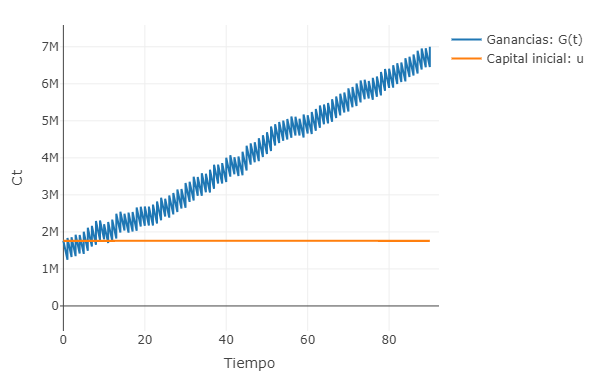
\includegraphics[width=0.8\textwidth,height=\textheight]{fig-trayectoriapdf.png}

}

\caption{\label{fig-fig-trayectoriapdf}Trayectoria del proceso de
evolución del modelo modificado de Cramér Lundberg antes de la
pandemia.}

\end{figure}%

\subsubsection{Probabilidad de ruina}\label{probabilidad-de-ruina}

Con la simulación de la variable aleatoria \(G(t)\), es posible ahora
calcular la probabilidad de ruina, utilizando el método de Monte
Carlo(citar).

Para ello, se quiere analizar el momento en el que \(G(t)\leq u\), es
decir cuando la ganancia al final de la semana \(t\) es menor al capital
inicial. Cuando \(G(t)\leq0\), se alcanza como la ruina de la empresa,
para ambos casos se utiliza la comparación con la tasa de interés para
préstamos bancarios de \(0.8\) anual.

El código para simular la probabilidad de las ganancias finales bajas es
el siguiente:

\begin{Shaded}
\begin{Highlighting}[]
\CommentTok{\#Simulación de la probabilidad de ruina: Antes de la pandemia}
\CommentTok{\#Con los datos reales de la empresa}
\FunctionTok{library}\NormalTok{(dplyr) }\CommentTok{\# librería para poder renombrar }
\CommentTok{\#las cabeceras de los dataframes}

\CommentTok{\#Parámetros}
\FunctionTok{set.seed}\NormalTok{(}\DecValTok{13}\NormalTok{) }\CommentTok{\#semilla fija}
\NormalTok{u }\OtherTok{=} \DecValTok{1759629} \CommentTok{\#surplus(capital inicial de salvamento)}
\CommentTok{\#Es un estimado a partir de la media de las ganancias por semana, }
\CommentTok{\#multiplicado por 10/3, }
\CommentTok{\#siendo una proporción para evitar la ruina}
\CommentTok{\# u (sum(medias))*(10/3)}
\NormalTok{c }\OtherTok{=} \FloatTok{0.29}\SpecialCharTok{*}\NormalTok{u }\CommentTok{\#prima de pago cada tiempo t. c=0.5*u}
\NormalTok{lambda\_Nt }\OtherTok{=} \FloatTok{0.5}
\CommentTok{\#lambda\_Xi = 3}
\NormalTok{t\_final }\OtherTok{=} \DecValTok{48}
\NormalTok{mu }\OtherTok{=} \DecValTok{1} \CommentTok{\#tiempos entrellegadas constantes}
\NormalTok{trayectoria\_CLt }\OtherTok{\textless{}{-}} \ControlFlowTok{function}\NormalTok{(u, c, lambda\_Nt, t\_final)}
\NormalTok{\{}
\NormalTok{  tiempo }\OtherTok{\textless{}{-}} \FunctionTok{c}\NormalTok{(}\DecValTok{0}\NormalTok{)}
\NormalTok{  Cramer\_trayectoria }\OtherTok{\textless{}{-}} \FunctionTok{c}\NormalTok{(u)}
  \ControlFlowTok{while}\NormalTok{(tiempo[}\FunctionTok{length}\NormalTok{(tiempo)] }\SpecialCharTok{\textless{}}\NormalTok{ t\_final)}
\NormalTok{  \{}
\NormalTok{    tiempo\_llegada }\OtherTok{\textless{}{-}}\NormalTok{ (}\DecValTok{1}\NormalTok{) }
    \CommentTok{\#Suponiendo los tiempos entrellegadas constantes \textbackslash{}mu = 1}
\NormalTok{    Y\_i }\OtherTok{\textless{}{-}}\NormalTok{  (}\FunctionTok{rnorm}\NormalTok{(}\DecValTok{1}\NormalTok{, }\AttributeTok{mean =} \FloatTok{139929.468}\NormalTok{, }\AttributeTok{sd =} \FloatTok{24521.524}\NormalTok{ ) }\SpecialCharTok{+} 
             \FunctionTok{rnorm}\NormalTok{(}\DecValTok{1}\NormalTok{, }\AttributeTok{mean =} \FloatTok{48125.734}\NormalTok{ , }\AttributeTok{sd=}\FloatTok{17150.338}\NormalTok{ ) }\SpecialCharTok{+}  
             \FunctionTok{rnorm}\NormalTok{(}\DecValTok{1}\NormalTok{, }\AttributeTok{mean =}  \FloatTok{44509.755}\NormalTok{, }\AttributeTok{sd =} \FloatTok{14312.338}\NormalTok{ ) }\SpecialCharTok{+} 
             \FunctionTok{rnorm}\NormalTok{(}\DecValTok{1}\NormalTok{, }\AttributeTok{mean =}   \FloatTok{46904.516}\NormalTok{, }\AttributeTok{sd =} \FloatTok{16238.151}\NormalTok{ ) }\SpecialCharTok{+} 
             \FunctionTok{rnorm}\NormalTok{(}\DecValTok{1}\NormalTok{, }\AttributeTok{mean =} \FloatTok{52786.734}\NormalTok{  , }\AttributeTok{sd =} \FloatTok{18403.17}\NormalTok{ ) }\SpecialCharTok{+} 
             \FunctionTok{rnorm}\NormalTok{(}\DecValTok{1}\NormalTok{, }\AttributeTok{mean =} \FloatTok{118645.9}\NormalTok{  , }\AttributeTok{sd =} \FloatTok{36530.24}\NormalTok{) }\SpecialCharTok{+}
             \FunctionTok{rweibull}\NormalTok{(}\DecValTok{1}\NormalTok{,  }\AttributeTok{shape =} \FloatTok{4.784508e+00}\NormalTok{, }\AttributeTok{scale =} \FloatTok{1.295070e+05}\NormalTok{)) }
\NormalTok{    tiempo }\OtherTok{\textless{}{-}} \FunctionTok{c}\NormalTok{(tiempo, tiempo[}\FunctionTok{length}\NormalTok{(tiempo)] }\SpecialCharTok{+}
\NormalTok{                  tiempo\_llegada,tiempo[}\FunctionTok{length}\NormalTok{(tiempo)] }\SpecialCharTok{+} 
\NormalTok{                  tiempo\_llegada ) }
\NormalTok{    Cramer\_trayectoria }\OtherTok{\textless{}{-}}\FunctionTok{c}\NormalTok{(Cramer\_trayectoria,}
\NormalTok{                Cramer\_trayectoria[}\FunctionTok{length}\NormalTok{(Cramer\_trayectoria)]}\SpecialCharTok{{-}}
\NormalTok{                  c}\SpecialCharTok{*}\NormalTok{tiempo\_llegada,}
\NormalTok{                Cramer\_trayectoria[}\FunctionTok{length}\NormalTok{(Cramer\_trayectoria)]}\SpecialCharTok{{-}}
\NormalTok{                  c}\SpecialCharTok{*}\NormalTok{tiempo\_llegada }\SpecialCharTok{+}\NormalTok{  Y\_i )}
    \ControlFlowTok{if}\NormalTok{(Cramer\_trayectoria[}\FunctionTok{length}\NormalTok{(Cramer\_trayectoria)] }\SpecialCharTok{\textless{}} \DecValTok{0}\NormalTok{)\{}
\NormalTok{      ruina }\OtherTok{=} \DecValTok{1}
\NormalTok{    \}}
    \ControlFlowTok{else}\NormalTok{\{}
\NormalTok{      ruina }\OtherTok{=} \DecValTok{0}
\NormalTok{    \}}
\NormalTok{  \}}
\CommentTok{\# 1.08*u es la ganancia inferior a la de un tasa de }
  \CommentTok{\#un título financiero }
\CommentTok{\#para el año 2018}
  \ControlFlowTok{if}\NormalTok{(Cramer\_trayectoria[}\FunctionTok{length}\NormalTok{(Cramer\_trayectoria)] }\SpecialCharTok{\textless{}} \FloatTok{1.08}\SpecialCharTok{*}\NormalTok{u) \{}
\NormalTok{    ganancia\_no\_deseada }\OtherTok{=} \DecValTok{1}
    
\NormalTok{  \} }
  \ControlFlowTok{else}\NormalTok{\{}
\NormalTok{    ganancia\_no\_deseada }\OtherTok{=} \DecValTok{0}
\NormalTok{  \}}
\NormalTok{  df }\OtherTok{\textless{}{-}} \FunctionTok{data.frame}\NormalTok{(tiempo, Cramer\_trayectoria)}
\NormalTok{  df\_trayectoria }\OtherTok{\textless{}{-}} \FunctionTok{data.frame}\NormalTok{(df}\SpecialCharTok{\%\textgreater{}\%}\NormalTok{rename}
\NormalTok{                               (}\AttributeTok{Tiempo =}\NormalTok{ tiempo, }
                                \AttributeTok{Ct =}\NormalTok{ Cramer\_trayectoria))}
\NormalTok{  salida }\OtherTok{\textless{}{-}} \FunctionTok{c}\NormalTok{(ruina, ganancia\_no\_deseada)}
  \FunctionTok{return}\NormalTok{(salida)}
  
\NormalTok{\}}
\NormalTok{trayectoria }\OtherTok{\textless{}{-}} \FunctionTok{trayectoria\_CLt}\NormalTok{(u,c,lambda\_Nt, t\_final )}
\CommentTok{\#Método de monte carlo para estimar }
\CommentTok{\#la probabilidad de las ganancias bajas}
\NormalTok{n\_replicaciones }\OtherTok{=} \DecValTok{100}
\NormalTok{r\_baja\_ganancia }\OtherTok{\textless{}{-}} \FunctionTok{replicate}\NormalTok{(n\_replicaciones,}
\FunctionTok{trayectoria\_CLt}\NormalTok{(u, c, lambda\_Nt, t\_final)}
\NormalTok{[}\DecValTok{2}\NormalTok{])}
\CommentTok{\#r\_baja\_ganancia }
\NormalTok{prob\_baja\_ganancia }\OtherTok{\textless{}{-}} \FunctionTok{sum}\NormalTok{(r\_baja\_ganancia }\SpecialCharTok{\textgreater{}}\DecValTok{0}\NormalTok{)}\SpecialCharTok{/}\NormalTok{n\_replicaciones}
\end{Highlighting}
\end{Shaded}

Es claro que la evolución de \(G(t)\) antes de la pandemia genera una
probabilidad de ganancias bajas cero.

\begin{verbatim}
[1] 0
\end{verbatim}

El código para calcular la probabilidad de ruina es el siguiente:

\begin{Shaded}
\begin{Highlighting}[]
\CommentTok{\#Simulación de la probabilidad de ruina: Antes de la pandemia}
\CommentTok{\#Con los datos reales de la empresa}
\FunctionTok{library}\NormalTok{(dplyr) }\CommentTok{\# libreria para poder renombrar }
\CommentTok{\#las cabeceras de los dataframes}

\CommentTok{\#Parametros}
\FunctionTok{set.seed}\NormalTok{(}\DecValTok{13}\NormalTok{) }\CommentTok{\#semilla fija}
\NormalTok{u }\OtherTok{=} \DecValTok{1759629} \CommentTok{\#surplus(capital inicial de salvamento)}
\CommentTok{\#Es un estimado a partir de la media de las ganancias por semana, }
\CommentTok{\#multiplicado por 10/3, }
\CommentTok{\#siendo una proporción para evitar la ruina}
\CommentTok{\# u (sum(medias))*(10/3)}
\NormalTok{c }\OtherTok{=} \FloatTok{0.29}\SpecialCharTok{*}\NormalTok{u }\CommentTok{\#prima de pago cada tiempo t. c=0.5*u}
\NormalTok{lambda\_Nt }\OtherTok{=} \FloatTok{0.5}
\CommentTok{\#lambda\_Xi = 3}
\NormalTok{t\_final }\OtherTok{=} \DecValTok{48}
\NormalTok{mu }\OtherTok{=} \DecValTok{1} \CommentTok{\#tiempos entrellegadas constantes}
\NormalTok{trayectoria\_CLt }\OtherTok{\textless{}{-}} \ControlFlowTok{function}\NormalTok{(u, c, lambda\_Nt, t\_final)}
\NormalTok{\{}
\NormalTok{  tiempo }\OtherTok{\textless{}{-}} \FunctionTok{c}\NormalTok{(}\DecValTok{0}\NormalTok{)}
\NormalTok{  Cramer\_trayectoria }\OtherTok{\textless{}{-}} \FunctionTok{c}\NormalTok{(u)}
  \ControlFlowTok{while}\NormalTok{(tiempo[}\FunctionTok{length}\NormalTok{(tiempo)] }\SpecialCharTok{\textless{}}\NormalTok{ t\_final)}
\NormalTok{  \{}
\NormalTok{    tiempo\_llegada }\OtherTok{\textless{}{-}}\NormalTok{ (}\DecValTok{1}\NormalTok{) }
\CommentTok{\#Suponiendo los tiempos entrellegadas constantes \textbackslash{}mu = 1}
\NormalTok{    Y\_i }\OtherTok{\textless{}{-}}\NormalTok{  (}\FunctionTok{rnorm}\NormalTok{(}\DecValTok{1}\NormalTok{, }\AttributeTok{mean =} \FloatTok{139929.468}\NormalTok{, }\AttributeTok{sd =} \FloatTok{24521.524}\NormalTok{ ) }\SpecialCharTok{+}
             \FunctionTok{rnorm}\NormalTok{(}\DecValTok{1}\NormalTok{, }\AttributeTok{mean =} \FloatTok{48125.734}\NormalTok{ , }\AttributeTok{sd=}\FloatTok{17150.338}\NormalTok{ )   }\SpecialCharTok{+}  
             \FunctionTok{rnorm}\NormalTok{(}\DecValTok{1}\NormalTok{, }\AttributeTok{mean =}  \FloatTok{44509.755}\NormalTok{, }\AttributeTok{sd =} \FloatTok{14312.338}\NormalTok{ ) }\SpecialCharTok{+} 
             \FunctionTok{rnorm}\NormalTok{(}\DecValTok{1}\NormalTok{, }\AttributeTok{mean =}   \FloatTok{46904.516}\NormalTok{, }\AttributeTok{sd =} \FloatTok{16238.151}\NormalTok{) }\SpecialCharTok{+} 
             \FunctionTok{rnorm}\NormalTok{(}\DecValTok{1}\NormalTok{, }\AttributeTok{mean =} \FloatTok{52786.734}\NormalTok{  , }\AttributeTok{sd =} \FloatTok{18403.17}\NormalTok{ ) }\SpecialCharTok{+}
             \FunctionTok{rnorm}\NormalTok{(}\DecValTok{1}\NormalTok{, }\AttributeTok{mean =} \FloatTok{118645.9}\NormalTok{  , }\AttributeTok{sd =} \FloatTok{36530.24}\NormalTok{)   }\SpecialCharTok{+} 
             \FunctionTok{rweibull}\NormalTok{(}\DecValTok{1}\NormalTok{,  }\AttributeTok{shape =} \FloatTok{4.784508e+00}\NormalTok{, }\AttributeTok{scale =} \FloatTok{1.295070e+05}\NormalTok{)) }
\NormalTok{    tiempo }\OtherTok{\textless{}{-}} \FunctionTok{c}\NormalTok{(tiempo, tiempo[}\FunctionTok{length}\NormalTok{(tiempo)] }\SpecialCharTok{+}
\NormalTok{                  tiempo\_llegada,tiempo[}\FunctionTok{length}\NormalTok{(tiempo)] }\SpecialCharTok{+} 
\NormalTok{                  tiempo\_llegada ) }
\NormalTok{    Cramer\_trayectoria }\OtherTok{\textless{}{-}}\FunctionTok{c}\NormalTok{(Cramer\_trayectoria,}
\NormalTok{                Cramer\_trayectoria[}\FunctionTok{length}\NormalTok{(Cramer\_trayectoria)]}\SpecialCharTok{{-}}
\NormalTok{                             c}\SpecialCharTok{*}\NormalTok{tiempo\_llegada,}
\NormalTok{                Cramer\_trayectoria[}\FunctionTok{length}\NormalTok{(Cramer\_trayectoria)]}\SpecialCharTok{{-}}
\NormalTok{                             c}\SpecialCharTok{*}\NormalTok{tiempo\_llegada }\SpecialCharTok{+}\NormalTok{  Y\_i )}
    \ControlFlowTok{if}\NormalTok{(Cramer\_trayectoria[}\FunctionTok{length}\NormalTok{(Cramer\_trayectoria)] }\SpecialCharTok{\textless{}} \DecValTok{0}\NormalTok{)\{}
\NormalTok{      ruina }\OtherTok{=} \DecValTok{1}
\NormalTok{    \}}
    \ControlFlowTok{else}\NormalTok{\{}
\NormalTok{      ruina }\OtherTok{=} \DecValTok{0}
\NormalTok{    \}}
\NormalTok{  \}}
\CommentTok{\# 1.08*u es la ganancia inferior a la de un tasa de}
\CommentTok{\# un título financiero para el año 2018}
  \ControlFlowTok{if}\NormalTok{(Cramer\_trayectoria[}\FunctionTok{length}\NormalTok{(Cramer\_trayectoria)] }\SpecialCharTok{\textless{}} \FloatTok{1.08}\SpecialCharTok{*}\NormalTok{u) \{}
\NormalTok{    ganancia\_no\_deseada }\OtherTok{=} \DecValTok{1}
    
\NormalTok{  \} }
  \ControlFlowTok{else}\NormalTok{\{}
\NormalTok{    ganancia\_no\_deseada }\OtherTok{=} \DecValTok{0}
\NormalTok{  \}}
\NormalTok{  df }\OtherTok{\textless{}{-}} \FunctionTok{data.frame}\NormalTok{(tiempo, Cramer\_trayectoria)}
\NormalTok{  df\_trayectoria }\OtherTok{\textless{}{-}} \FunctionTok{data.frame}\NormalTok{(df}\SpecialCharTok{\%\textgreater{}\%}\NormalTok{ rename}
\NormalTok{                               (}\AttributeTok{Tiempo =}\NormalTok{ tiempo, }
                                 \AttributeTok{Ct =}\NormalTok{ Cramer\_trayectoria))}
\NormalTok{  salida }\OtherTok{\textless{}{-}} \FunctionTok{c}\NormalTok{(ruina, ganancia\_no\_deseada)}
  \FunctionTok{return}\NormalTok{(salida)}
  
\NormalTok{\}}
\NormalTok{trayectoria }\OtherTok{\textless{}{-}} \FunctionTok{trayectoria\_CLt}\NormalTok{(u,c,lambda\_Nt, t\_final )}
\CommentTok{\#Método de monte carlo para estimar la probabilidad de ruina}
\NormalTok{n\_replicaciones }\OtherTok{=} \DecValTok{100}
\NormalTok{r\_ruina }\OtherTok{\textless{}{-}} \FunctionTok{replicate}\NormalTok{(n\_replicaciones, }
            \FunctionTok{trayectoria\_CLt}\NormalTok{(u, c, lambda\_Nt, t\_final)[}\DecValTok{1}\NormalTok{])}
\CommentTok{\#r\_ruina}
\NormalTok{prob\_ruin }\OtherTok{\textless{}{-}} \FunctionTok{sum}\NormalTok{(r\_ruina}\SpecialCharTok{\textgreater{}}\DecValTok{0}\NormalTok{)}\SpecialCharTok{/}\NormalTok{n\_replicaciones}
\end{Highlighting}
\end{Shaded}

En efecto la evolución de \(G(t)\) antes de la pandemia genera una
probabilidad ruina cero.

\begin{verbatim}
[1] 0
\end{verbatim}

\subsubsection{Análisis de
sensibilidad}\label{anuxe1lisis-de-sensibilidad}

Se desea ahora analizar los cambios del resultado del modelo cuando se
modifican sus entradas o parámetros, por lo cual se realiza un análisis
de sensibilidad de algunos parámetros.

Para ello del modelo modificado de Cramér Lundberg se toma los
parámetros \(u\) y \(c\) del modelo modificado y se establece los rangos
o valores posibles para cada uno de los ciertos parámetros, también se
toma las medianas de las ganancia en la semana final de 100 simulaciones
de las trayectorias del modelo, los rangos se determinan hasta que el
modelo presente un comportamiento diferente.

\begin{Shaded}
\begin{Highlighting}[]
\CommentTok{\#Simulación Modelo Clásico de Cramer{-}Lundberg para tres meses: }
\CommentTok{\#Antes de la pandemia Con los datos reales de la empresa}

\FunctionTok{library}\NormalTok{(dplyr) }\CommentTok{\# libreria para poder renombrar }
\CommentTok{\#las cabeceras de los dataframes}
\CommentTok{\#Parametros}
\FunctionTok{set.seed}\NormalTok{(}\DecValTok{13}\NormalTok{) }\CommentTok{\#semilla fija}
\NormalTok{u }\OtherTok{=} \DecValTok{1759629} \CommentTok{\#surplus(capital inicial de salvamento)}
\CommentTok{\#Es un estimado a partir de la media de las ganancias por semana, }
\CommentTok{\#multiplicado por 10/3, }
\CommentTok{\#siendo una proporción para evitar la ruina}
\CommentTok{\# u (sum(medias))*(10/3)}
\NormalTok{decimal\_c }\OtherTok{=} \FloatTok{0.29}
\NormalTok{c }\OtherTok{=}\NormalTok{decimal\_c}\SpecialCharTok{*}\NormalTok{u }\CommentTok{\#prima de pago cada timepo t. c=0.5*u}
\NormalTok{lambda\_Nt }\OtherTok{=} \FloatTok{0.5}
\CommentTok{\#lambda\_Xi = 3}
\NormalTok{t\_final }\OtherTok{=} \DecValTok{90}
\CommentTok{\# S(t) = \textbackslash{}sum\_\{i=1\}\^{}\{N(t)\}X\_i}
\CommentTok{\#donde N(t)\textasciitilde{} Poisson (lambda*t)}
\CommentTok{\# X\_i \textasciitilde{} exponencial (lambda\_Xi)}
\CommentTok{\#CL = REPRESENTA EL MODELO DE CRAMER LUNDBERG}
\CommentTok{\#Simulación de trayectoria de CL\_t, cuando t \textless{} t\_final.}
\NormalTok{trayectoria\_CLt }\OtherTok{\textless{}{-}} \ControlFlowTok{function}\NormalTok{(u, c, lambda\_Nt, t\_final)}
\NormalTok{\{}
\NormalTok{  tiempo }\OtherTok{\textless{}{-}} \FunctionTok{c}\NormalTok{(}\DecValTok{0}\NormalTok{)}
\NormalTok{  Cramer\_trayectoria }\OtherTok{\textless{}{-}} \FunctionTok{c}\NormalTok{(u)}
  \ControlFlowTok{while}\NormalTok{(tiempo[}\FunctionTok{length}\NormalTok{(tiempo)] }\SpecialCharTok{\textless{}}\NormalTok{ t\_final)}
\NormalTok{  \{}
    \CommentTok{\#tiempo\_llegada \textless{}{-} rexp(1, rate = lambda\_Nt)}
\NormalTok{    tiempo\_llegada }\OtherTok{\textless{}{-}}\NormalTok{ (}\DecValTok{1}\NormalTok{)}
\NormalTok{    Y\_i }\OtherTok{\textless{}{-}}\NormalTok{  (}\FunctionTok{rnorm}\NormalTok{(}\DecValTok{1}\NormalTok{, }\AttributeTok{mean =} \FloatTok{139929.468}\NormalTok{, }\AttributeTok{sd =} \FloatTok{24521.524}\NormalTok{ ) }\SpecialCharTok{+}
            \FunctionTok{rnorm}\NormalTok{(}\DecValTok{1}\NormalTok{, }\AttributeTok{mean =} \FloatTok{48125.734}\NormalTok{ , }\AttributeTok{sd=}\FloatTok{17150.338}\NormalTok{ )    }\SpecialCharTok{+}  
            \FunctionTok{rnorm}\NormalTok{(}\DecValTok{1}\NormalTok{, }\AttributeTok{mean =}  \FloatTok{44509.755}\NormalTok{, }\AttributeTok{sd =} \FloatTok{14312.338}\NormalTok{ )  }\SpecialCharTok{+} 
            \FunctionTok{rnorm}\NormalTok{(}\DecValTok{1}\NormalTok{, }\AttributeTok{mean =}   \FloatTok{46904.516}\NormalTok{, }\AttributeTok{sd =} \FloatTok{16238.151}\NormalTok{ ) }\SpecialCharTok{+} 
            \FunctionTok{rnorm}\NormalTok{(}\DecValTok{1}\NormalTok{, }\AttributeTok{mean =} \FloatTok{52786.734}\NormalTok{  , }\AttributeTok{sd =} \FloatTok{18403.17}\NormalTok{ )  }\SpecialCharTok{+} 
            \FunctionTok{rnorm}\NormalTok{(}\DecValTok{1}\NormalTok{, }\AttributeTok{mean =} \FloatTok{81601.876}\NormalTok{  , }\AttributeTok{sd =} \FloatTok{23756.037}\NormalTok{)  }\SpecialCharTok{+} 
            \FunctionTok{rweibull}\NormalTok{(}\DecValTok{1}\NormalTok{,  }\AttributeTok{shape =} \FloatTok{4.784508e+00}\NormalTok{, }\AttributeTok{scale =} \FloatTok{1.295070e+05}\NormalTok{ )) }
\NormalTok{    tiempo }\OtherTok{\textless{}{-}} \FunctionTok{c}\NormalTok{(tiempo, tiempo[}\FunctionTok{length}\NormalTok{(tiempo)] }\SpecialCharTok{+}
\NormalTok{                  tiempo\_llegada,}
\NormalTok{                tiempo[}\FunctionTok{length}\NormalTok{(tiempo)] }\SpecialCharTok{+} 
\NormalTok{                  tiempo\_llegada ) }
\NormalTok{    Cramer\_trayectoria }\OtherTok{\textless{}{-}} \FunctionTok{c}\NormalTok{(Cramer\_trayectoria,}
\NormalTok{            Cramer\_trayectoria[}\FunctionTok{length}\NormalTok{(Cramer\_trayectoria)]}\SpecialCharTok{{-}} 
\NormalTok{                          c}\SpecialCharTok{*}\NormalTok{tiempo\_llegada,}
\NormalTok{            Cramer\_trayectoria[}\FunctionTok{length}\NormalTok{(Cramer\_trayectoria)]}\SpecialCharTok{{-}}
\NormalTok{                          c}\SpecialCharTok{*}\NormalTok{tiempo\_llegada }\SpecialCharTok{+}\NormalTok{  Y\_i )}
    \ControlFlowTok{if}\NormalTok{(Cramer\_trayectoria[}\FunctionTok{length}\NormalTok{(Cramer\_trayectoria)] }\SpecialCharTok{\textless{}} \DecValTok{0}\NormalTok{)}
\NormalTok{      \{}
\NormalTok{      ruina }\OtherTok{=} \DecValTok{1}
\NormalTok{      \}}
    \ControlFlowTok{else}
\NormalTok{      \{}
\NormalTok{      ruina }\OtherTok{=} \DecValTok{0}
\NormalTok{      \}}
\NormalTok{  \}}
\NormalTok{  df }\OtherTok{\textless{}{-}} \FunctionTok{data.frame}\NormalTok{(tiempo, Cramer\_trayectoria)}
\NormalTok{  df\_trayectoria }\OtherTok{\textless{}{-}} \FunctionTok{data.frame}\NormalTok{(df}\SpecialCharTok{\%\textgreater{}\%}\NormalTok{ rename}
\NormalTok{                               (}\AttributeTok{Tiempo =}\NormalTok{ tiempo, }
                                \AttributeTok{Ct =}\NormalTok{ Cramer\_trayectoria))}
  \FunctionTok{return}\NormalTok{(df\_trayectoria}\SpecialCharTok{$}\NormalTok{Ct[}\FunctionTok{length}\NormalTok{(df\_trayectoria}\SpecialCharTok{$}\NormalTok{Ct)])}
  
\NormalTok{\}}

\CommentTok{\# La función generador\_mediana nos calcula }
\CommentTok{\#la mediana de las ganancias finales }
\CommentTok{\#de 100 trayectorias, fijando el u= surplus y el c}
\NormalTok{generador\_mediana}\OtherTok{\textless{}{-}} \ControlFlowTok{function}\NormalTok{(ui,cj)}
\NormalTok{  \{}
\NormalTok{  ganancia\_final\_replicas }\OtherTok{\textless{}{-}} \FunctionTok{replicate}\NormalTok{(}\DecValTok{100}\NormalTok{, }
                                       \FunctionTok{trayectoria\_CLt}\NormalTok{(u, c,}
\NormalTok{                                        lambda\_Nt, t\_final))}
  \FunctionTok{return}\NormalTok{( }\FunctionTok{median}\NormalTok{(ganancia\_final\_replicas))}
\NormalTok{  \}}
\CommentTok{\#Se crea la rejilla donde se hace el analisis de sensibilidad}
\CommentTok{\#para diferentes valores de u y c}
\NormalTok{grid\_u }\OtherTok{\textless{}{-}} \FunctionTok{seq}\NormalTok{(}\AttributeTok{from =}\NormalTok{ (u}\DecValTok{{-}100000}\SpecialCharTok{*}\DecValTok{4}\NormalTok{), }\AttributeTok{to =}\NormalTok{ (u}\SpecialCharTok{+}\DecValTok{100000}\SpecialCharTok{*}\DecValTok{4}\NormalTok{), }\AttributeTok{by =} \DecValTok{100000}\NormalTok{)}
\NormalTok{grid\_c }\OtherTok{\textless{}{-}} \FunctionTok{seq}\NormalTok{(}\AttributeTok{from =}\NormalTok{ (decimal\_c}\FloatTok{{-}0.01}\SpecialCharTok{*}\DecValTok{4}\NormalTok{), }\AttributeTok{to =}\NormalTok{ (decimal\_c}\FloatTok{+0.01}\SpecialCharTok{*}\DecValTok{4}\NormalTok{), }
              \AttributeTok{by =} \FloatTok{0.01}\NormalTok{)}
\NormalTok{u\_t }\OtherTok{\textless{}{-}}\NormalTok{ grid\_u}

\NormalTok{matriz\_mediana }\OtherTok{\textless{}{-}} \FunctionTok{matrix}\NormalTok{(}\FunctionTok{rep}\NormalTok{(}\DecValTok{0}\NormalTok{, }\FunctionTok{length}\NormalTok{(grid\_u)}\SpecialCharTok{*}\FunctionTok{length}\NormalTok{(grid\_c)),}
\AttributeTok{nrow=} \FunctionTok{length}\NormalTok{(grid\_u), }\AttributeTok{ncol=} \FunctionTok{length}\NormalTok{(grid\_c))}
\NormalTok{G\_t }\OtherTok{\textless{}{-}}\NormalTok{ matriz\_mediana}
\ControlFlowTok{for}\NormalTok{ (i }\ControlFlowTok{in} \DecValTok{1}\SpecialCharTok{:}\FunctionTok{length}\NormalTok{(grid\_u)) }
\NormalTok{  \{}
    \ControlFlowTok{for}\NormalTok{ (j }\ControlFlowTok{in} \DecValTok{1}\SpecialCharTok{:}\FunctionTok{length}\NormalTok{(grid\_c)) }
\NormalTok{      \{}
\NormalTok{        G\_t[i,j] }\OtherTok{\textless{}{-}} \FunctionTok{generador\_mediana}\NormalTok{(u\_t[i],}
\NormalTok{                              grid\_c[j]}\SpecialCharTok{*}\NormalTok{u\_t[i])}
\NormalTok{      \}}
\NormalTok{  \}  }
\CommentTok{\#matriz\_mediana}

\CommentTok{\#Grafica del ánalisis de sensibilidad}
\FunctionTok{library}\NormalTok{(plotly)}
\FunctionTok{library}\NormalTok{(ggplot2)}
\NormalTok{c\_t }\OtherTok{\textless{}{-}}\NormalTok{ grid\_u}\SpecialCharTok{*}\NormalTok{grid\_c}
\NormalTok{fig }\OtherTok{\textless{}{-}} \FunctionTok{plot\_ly}\NormalTok{(}
  \AttributeTok{type =} \StringTok{\textquotesingle{}surface\textquotesingle{}}\NormalTok{,}
  \AttributeTok{contours =} \FunctionTok{list}\NormalTok{(}
    \AttributeTok{x =} \FunctionTok{list}\NormalTok{(}\AttributeTok{show =} \ConstantTok{TRUE}\NormalTok{, }\AttributeTok{start =}\NormalTok{ u\_t[}\DecValTok{1}\NormalTok{], }
             \AttributeTok{end =}\NormalTok{ u\_t[}\FunctionTok{length}\NormalTok{(u\_t)], }
             \AttributeTok{size =}\DecValTok{100000}\NormalTok{ , }\AttributeTok{color =} \StringTok{\textquotesingle{}red\textquotesingle{}}\NormalTok{),}
    \AttributeTok{z =} \FunctionTok{list}\NormalTok{(}\AttributeTok{show =} \ConstantTok{TRUE}\NormalTok{, }\AttributeTok{start =}\NormalTok{ G\_t[}\DecValTok{1}\NormalTok{], }
             \AttributeTok{end =}\NormalTok{ G\_t[}\FunctionTok{length}\NormalTok{(G\_t)], }
             \AttributeTok{size =} \FloatTok{0.01}\SpecialCharTok{*}\DecValTok{100000}\NormalTok{)),}
  \AttributeTok{x =} \SpecialCharTok{\textasciitilde{}}\NormalTok{u\_t,}
  \AttributeTok{y =} \SpecialCharTok{\textasciitilde{}}\NormalTok{c\_t,}
  \AttributeTok{z =} \SpecialCharTok{\textasciitilde{}}\NormalTok{G\_t)}
\NormalTok{fig }\OtherTok{\textless{}{-}}\NormalTok{ fig }\SpecialCharTok{\%\textgreater{}\%} \FunctionTok{layout}\NormalTok{(}
  \AttributeTok{scene =} \FunctionTok{list}\NormalTok{(}\AttributeTok{autosize =}\NormalTok{ F, }\AttributeTok{width =} \DecValTok{500}\NormalTok{, }\AttributeTok{height =} \DecValTok{500}\NormalTok{,}
    \AttributeTok{xaxis =} \FunctionTok{list}\NormalTok{(}\AttributeTok{nticks =} \DecValTok{20}\NormalTok{),}
    \AttributeTok{zaxis =} \FunctionTok{list}\NormalTok{(}\AttributeTok{nticks =} \DecValTok{8}\NormalTok{),}
    \AttributeTok{camera =} \FunctionTok{list}\NormalTok{(}\AttributeTok{eye =} \FunctionTok{list}\NormalTok{(}\AttributeTok{x =} \DecValTok{0}\NormalTok{, }
                             \AttributeTok{y =} \SpecialCharTok{{-}}\DecValTok{1}\NormalTok{, }\AttributeTok{z =} \DecValTok{1}\NormalTok{)),}
    \AttributeTok{aspectratio =} \FunctionTok{list}\NormalTok{(}\AttributeTok{x =}\NormalTok{ .}\DecValTok{9}\NormalTok{, }\AttributeTok{y =}\NormalTok{ .}\DecValTok{8}\NormalTok{, }\AttributeTok{z =} \FloatTok{0.2}\NormalTok{)))}

\NormalTok{fig}
\end{Highlighting}
\end{Shaded}

\begin{figure}[H]

{\centering 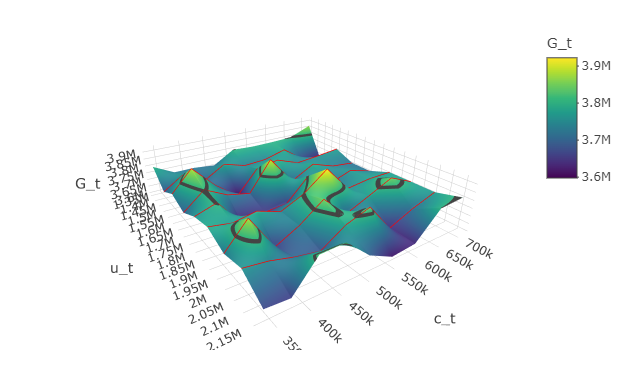
\includegraphics[width=5.20833in,height=\textheight]{fig-analisispdf.png}

}

\caption{Análisis de sensibilidad pre-pandemia para 90 semanas}

\end{figure}%

\subsection{Caso pos-pandemia}\label{caso-pos-pandemia}

De manera análoga a la metodología empleada con los datos
pre-pandemicos, para la simulación del modelo Crámer-Lundberg con los
datos después de la pandemia se hizo uso de las medias de las
distribuciones de las ventas por día tomado como las ganancias
acumuladas, y se estimó los parámetros de \(u\) y \(c\).

\subsubsection{Modelo de Cramér-Lundberg simulado en R con datos reales
de las ventas por día de la
empresa}\label{modelo-de-cramuxe9r-lundberg-simulado-en-r-con-datos-reales-de-las-ventas-por-duxeda-de-la-empresa}

En la (Figura~\ref{fig-fig-trayectoria2pdf}) se muestra la trayectoria
del modelo bajo los supuestos del modelo modificado, el proceso comienza
con \(t = 14\), que son las \(14\) semanas de de las ventas registradas
por día después del cierre pandemico, con un capital inicial de
\(u= 1759629\), una tasa de \(c= 0.29\), los montos de las ganancias
tienen todas distribución normal (\(N\)).

El código que genera la trayectoria es el siguiente:

\begin{Shaded}
\begin{Highlighting}[]
\FunctionTok{library}\NormalTok{(dplyr) }\CommentTok{\# libreria para poder renombrar }
\CommentTok{\#las cabeceras de los dataframes}
\CommentTok{\#Parametros}
\FunctionTok{set.seed}\NormalTok{(}\DecValTok{13}\NormalTok{) }\CommentTok{\#semilla fija}
\NormalTok{u }\OtherTok{=} \DecValTok{1759629} \CommentTok{\#surplus(capital inicial de salvamento)}
\CommentTok{\#Es un estimado a partir de la media de las ganancias por semana, }
\CommentTok{\#multiplicado por 10/3, }
\CommentTok{\#siendo una proporción para evitar la ruina}
\CommentTok{\# u (sum(medias))*(10/3)}
\NormalTok{c }\OtherTok{=}\NormalTok{ (}\FloatTok{0.29}\SpecialCharTok{*}\NormalTok{u) }\CommentTok{\#prima de pago cada timepo t. c=0.5*u}
\NormalTok{lambda\_Nt }\OtherTok{=} \FloatTok{0.5}
\CommentTok{\#lambda\_Xi = 3}
\NormalTok{t\_final }\OtherTok{=} \DecValTok{14}
\CommentTok{\# S(t) = \textbackslash{}sum\_\{i=1\}\^{}\{N(t)\}X\_i}
\CommentTok{\#donde N(t)\textasciitilde{} Poisson (lambda*t)}
\CommentTok{\# X\_i \textasciitilde{} exponencial (lambda\_Xi)}
\CommentTok{\#CL = REPRESENTA EL MODELO DE CRAMER LUNDBERG}
\CommentTok{\#Simulación de trayectoria de CL\_t, cuando t \textless{} t\_final.}
\NormalTok{trayectoria\_CLt\_post\_pandemia }\OtherTok{\textless{}{-}} \ControlFlowTok{function}\NormalTok{(u, c, lambda\_Nt, t\_final)}
\NormalTok{\{}
\NormalTok{  tiempo }\OtherTok{\textless{}{-}} \FunctionTok{c}\NormalTok{(}\DecValTok{0}\NormalTok{)}
\NormalTok{  Cramer\_trayectoria }\OtherTok{\textless{}{-}} \FunctionTok{c}\NormalTok{(u)}
  \ControlFlowTok{while}\NormalTok{(tiempo[}\FunctionTok{length}\NormalTok{(tiempo)] }\SpecialCharTok{\textless{}}\NormalTok{ t\_final)}
\NormalTok{  \{}
\NormalTok{    tiempo\_llegada }\OtherTok{\textless{}{-}}\NormalTok{ (}\DecValTok{1}\NormalTok{)}\CommentTok{\#rexp(1, rate = lambda\_Nt)}
\NormalTok{    Y\_i }\OtherTok{\textless{}{-}}\NormalTok{  (}\FunctionTok{rnorm}\NormalTok{(}\DecValTok{1}\NormalTok{, }\AttributeTok{mean =} \FloatTok{101919.050}\NormalTok{ , }\AttributeTok{sd =} \FloatTok{10877.075}\NormalTok{)}\SpecialCharTok{+}
             \FunctionTok{rnorm}\NormalTok{(}\DecValTok{1}\NormalTok{, }\AttributeTok{mean =}  \FloatTok{39841.721}\NormalTok{ , }\AttributeTok{sd=} \FloatTok{7873.446}\NormalTok{)  }\SpecialCharTok{+} 
             \FunctionTok{rnorm}\NormalTok{(}\DecValTok{1}\NormalTok{, }\AttributeTok{mean =}   \FloatTok{41751.747}\NormalTok{, }\AttributeTok{sd =} \FloatTok{5687.030}\NormalTok{) }\SpecialCharTok{+} 
             \FunctionTok{rnorm}\NormalTok{(}\DecValTok{1}\NormalTok{, }\AttributeTok{mean =}   \FloatTok{43243.143}\NormalTok{, }\AttributeTok{sd =} \FloatTok{10517.841}\NormalTok{)}\SpecialCharTok{+} 
             \FunctionTok{rnorm}\NormalTok{(}\DecValTok{1}\NormalTok{, }\AttributeTok{mean =} \FloatTok{43010.307}\NormalTok{  , }\AttributeTok{sd =} \FloatTok{7741.889}\NormalTok{ )}\SpecialCharTok{+} 
             \FunctionTok{rnorm}\NormalTok{(}\DecValTok{1}\NormalTok{, }\AttributeTok{mean =} \FloatTok{61191.300}\NormalTok{  , }\AttributeTok{sd =} \FloatTok{7202.989}\NormalTok{) }\SpecialCharTok{+} 
             \FunctionTok{rnorm}\NormalTok{(}\DecValTok{1}\NormalTok{, }\AttributeTok{mean =}  \FloatTok{85684.058}\NormalTok{ , }\AttributeTok{sd =} \FloatTok{8371.359}\NormalTok{ ) ) }
\NormalTok{tiempo }\OtherTok{\textless{}{-}} \FunctionTok{c}\NormalTok{(tiempo, tiempo[}\FunctionTok{length}\NormalTok{(tiempo)] }\SpecialCharTok{+}
\NormalTok{              tiempo\_llegada,tiempo[}\FunctionTok{length}\NormalTok{(tiempo)] }\SpecialCharTok{+}
\NormalTok{              tiempo\_llegada ) }
\NormalTok{Cramer\_trayectoria }\OtherTok{\textless{}{-}} \FunctionTok{c}\NormalTok{(Cramer\_trayectoria,}
\NormalTok{Cramer\_trayectoria[}\FunctionTok{length}\NormalTok{(Cramer\_trayectoria)] }\SpecialCharTok{{-}}
\NormalTok{  c}\SpecialCharTok{*}\NormalTok{tiempo\_llegada, }
\NormalTok{Cramer\_trayectoria[}\FunctionTok{length}\NormalTok{(Cramer\_trayectoria)] }\SpecialCharTok{{-}}
\NormalTok{  c}\SpecialCharTok{*}\NormalTok{tiempo\_llegada }\SpecialCharTok{+}\NormalTok{  Y\_i )}
\NormalTok{  \}}
\NormalTok{  df\_post\_pandemia }\OtherTok{\textless{}{-}} \FunctionTok{data.frame}\NormalTok{(tiempo, Cramer\_trayectoria)}
\NormalTok{df\_trayectoria\_post\_pandemia }\OtherTok{\textless{}{-}} \FunctionTok{data.frame}\NormalTok{(df\_post\_pandemia}\SpecialCharTok{\%\textgreater{}\%} 
                                        \FunctionTok{rename}\NormalTok{(}\AttributeTok{Tiempo =}\NormalTok{ tiempo,}
                                        \AttributeTok{Ct =}\NormalTok{ Cramer\_trayectoria))}
  \FunctionTok{return}\NormalTok{(df\_trayectoria\_post\_pandemia)}
\NormalTok{\}}
\NormalTok{trayectoria\_post\_pandemia }\OtherTok{\textless{}{-}} \FunctionTok{trayectoria\_CLt\_post\_pandemia}\NormalTok{(u,c,}
\NormalTok{                                              lambda\_Nt,t\_final)}


\FunctionTok{library}\NormalTok{(plotly)}
\NormalTok{fig\_tr2 }\OtherTok{\textless{}{-}} \FunctionTok{plot\_ly}\NormalTok{(trayectoria\_post\_pandemia, }\AttributeTok{x =} \SpecialCharTok{\textasciitilde{}}\NormalTok{Tiempo, }
                                              \AttributeTok{y =} \SpecialCharTok{\textasciitilde{}}\NormalTok{Ct, }
          \AttributeTok{name =} \StringTok{"Ganancias: G(t)"}\NormalTok{,}
          \AttributeTok{type =} \StringTok{"scatter"}\NormalTok{, }\AttributeTok{mode =} \StringTok{"lines"}\NormalTok{)}

\NormalTok{fig\_tr2 }\OtherTok{\textless{}{-}}\NormalTok{ fig\_tr2 }\SpecialCharTok{\%\textgreater{}\%} \FunctionTok{add\_trace}\NormalTok{(}\AttributeTok{x =} \SpecialCharTok{\textasciitilde{}}\NormalTok{Tiempo, }\AttributeTok{y =}\NormalTok{ u,}
        \AttributeTok{name =} \StringTok{"Capital inicial: u"}\NormalTok{, }
        \AttributeTok{type =} \StringTok{"scatter"}\NormalTok{, }\AttributeTok{mode =} \StringTok{"lines"}\NormalTok{)}
\NormalTok{fig\_tr2}
\end{Highlighting}
\end{Shaded}

\begin{figure}

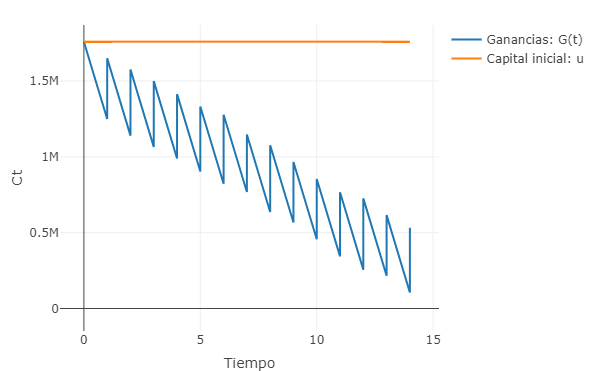
\includegraphics[width=6.25in,height=\textheight]{trayectoria2pdf.png}

\caption{\label{fig-fig-trayectoria2pdf}Trayectoria de pérdidas del
proceso de evolución modificado de Cramér Lundberg después de la
pandemia}

\end{figure}%

Se emplean los mismos parámetros obtenidos en el periodo de tiempo pre
pandemia del modelo modificado donde se observa una completa ruina al
alcanzar \(17\) semanas.

\begin{Shaded}
\begin{Highlighting}[]
\FunctionTok{library}\NormalTok{(dplyr) }\CommentTok{\# libreria para poder renombrar }
\CommentTok{\# las cabeceras de los dataframes}

\CommentTok{\#Parametros}
\FunctionTok{set.seed}\NormalTok{(}\DecValTok{13}\NormalTok{) }\CommentTok{\#semilla fija}
\NormalTok{u }\OtherTok{=} \DecValTok{1759629} \CommentTok{\#surplus(capital inicial de salvamento)}
\CommentTok{\#Es un estimado a partir de la media de las ganancias por semana, }
\CommentTok{\#multiplicado por 10/3, }
\CommentTok{\#siendo una proporción para evitar la ruina}
\CommentTok{\# u (sum(medias))*(10/3)}
\NormalTok{c }\OtherTok{=} \FloatTok{0.29}\SpecialCharTok{*}\NormalTok{u }\CommentTok{\#prima de pago cada timepo t. c=0.5*u}
\NormalTok{lambda\_Nt }\OtherTok{=} \FloatTok{0.5}
\CommentTok{\#lambda\_Xi = 3}
\NormalTok{t\_final }\OtherTok{=} \DecValTok{17}
\CommentTok{\# S(t) = \textbackslash{}sum\_\{i=1\}\^{}\{N(t)\}X\_i}
\CommentTok{\#donde N(t)\textasciitilde{} Poisson (lambda*t)}
\CommentTok{\# X\_i \textasciitilde{} exponencial (lambda\_Xi)}
\CommentTok{\#CL = REPRESENTA EL MODELO DE CRAMER LUNDBERG}
\CommentTok{\#Simulación de trayectoria de CL\_t, cuando t \textless{} t\_final.}
\NormalTok{trayectoria\_CLt\_post\_pandemia }\OtherTok{\textless{}{-}} \ControlFlowTok{function}\NormalTok{(u, c, lambda\_Nt, t\_final)}
\NormalTok{\{}
\NormalTok{  tiempo }\OtherTok{\textless{}{-}} \FunctionTok{c}\NormalTok{(}\DecValTok{0}\NormalTok{)}
\NormalTok{  Cramer\_trayectoria }\OtherTok{\textless{}{-}} \FunctionTok{c}\NormalTok{(u)}
  \ControlFlowTok{while}\NormalTok{(tiempo[}\FunctionTok{length}\NormalTok{(tiempo)] }\SpecialCharTok{\textless{}}\NormalTok{ t\_final)}
\NormalTok{  \{}
\NormalTok{    tiempo\_llegada }\OtherTok{\textless{}{-}}\NormalTok{ (}\DecValTok{1}\NormalTok{)}\CommentTok{\#rexp(1, rate = lambda\_Nt)}
\NormalTok{    Y\_i }\OtherTok{\textless{}{-}}\NormalTok{  (}\FunctionTok{rnorm}\NormalTok{(}\DecValTok{1}\NormalTok{, }\AttributeTok{mean =} \FloatTok{101919.050}\NormalTok{ , }\AttributeTok{sd =} \FloatTok{10877.075}\NormalTok{  ) }
\SpecialCharTok{+} \FunctionTok{rnorm}\NormalTok{(}\DecValTok{1}\NormalTok{, }\AttributeTok{mean =}  \FloatTok{39841.721}\NormalTok{ , }\AttributeTok{sd=} \FloatTok{7873.446} 
\NormalTok{    ) }\SpecialCharTok{+}  
\FunctionTok{rnorm}\NormalTok{(}\DecValTok{1}\NormalTok{, }\AttributeTok{mean =}   \FloatTok{41751.747}\NormalTok{, }\AttributeTok{sd =} \FloatTok{5687.030}\NormalTok{  ) }\SpecialCharTok{+} 
\FunctionTok{rnorm}\NormalTok{(}\DecValTok{1}\NormalTok{, }\AttributeTok{mean =}   \FloatTok{43243.143}\NormalTok{, }\AttributeTok{sd =} \FloatTok{10517.841}\NormalTok{ ) }\SpecialCharTok{+} 
\FunctionTok{rnorm}\NormalTok{(}\DecValTok{1}\NormalTok{, }\AttributeTok{mean =} \FloatTok{43010.307}\NormalTok{  , }\AttributeTok{sd =} \FloatTok{7741.889}\NormalTok{ ) }\SpecialCharTok{+} 
\FunctionTok{rnorm}\NormalTok{(}\DecValTok{1}\NormalTok{, }\AttributeTok{mean =} \FloatTok{61191.300}\NormalTok{  , }\AttributeTok{sd =} \FloatTok{7202.989}\NormalTok{) }\SpecialCharTok{+} 
\FunctionTok{rnorm}\NormalTok{(}\DecValTok{1}\NormalTok{, }\AttributeTok{mean =}  \FloatTok{85684.058}\NormalTok{ , }\AttributeTok{sd =} \FloatTok{8371.359}\NormalTok{ ) ) }
\NormalTok{    tiempo }\OtherTok{\textless{}{-}} \FunctionTok{c}\NormalTok{(tiempo, tiempo[}\FunctionTok{length}\NormalTok{(tiempo)] }
    \SpecialCharTok{+}\NormalTok{ tiempo\_llegada,tiempo[}\FunctionTok{length}\NormalTok{(tiempo)]}
    \SpecialCharTok{+}\NormalTok{ tiempo\_llegada ) }
\NormalTok{    Cramer\_trayectoria }\OtherTok{\textless{}{-}} \FunctionTok{c}\NormalTok{(Cramer\_trayectoria,}
\NormalTok{    Cramer\_trayectoria[}\FunctionTok{length}\NormalTok{(Cramer\_trayectoria)]}
    \SpecialCharTok{{-}}\NormalTok{ c}\SpecialCharTok{*}\NormalTok{tiempo\_llegada,}
\NormalTok{    Cramer\_trayectoria[}\FunctionTok{length}\NormalTok{(Cramer\_trayectoria)]}\SpecialCharTok{{-}}
\NormalTok{    c}\SpecialCharTok{*}\NormalTok{tiempo\_llegada }\SpecialCharTok{+}\NormalTok{  Y\_i )}
\NormalTok{  \}}
\NormalTok{  df\_post\_pandemia }\OtherTok{\textless{}{-}} \FunctionTok{data.frame}\NormalTok{(tiempo, Cramer\_trayectoria)}
\NormalTok{df\_trayectoria\_post\_pandemia }\OtherTok{\textless{}{-}} \FunctionTok{data.frame}\NormalTok{(df\_post\_pandemia}\SpecialCharTok{\%\textgreater{}\%}
                                        \FunctionTok{rename}\NormalTok{(}\AttributeTok{Tiempo =}\NormalTok{ tiempo,}
    \AttributeTok{Ct =}\NormalTok{ Cramer\_trayectoria))}
  \FunctionTok{return}\NormalTok{(df\_trayectoria\_post\_pandemia)}
\NormalTok{\}}
\NormalTok{trayectoria\_post\_pandemia }\OtherTok{\textless{}{-}} \FunctionTok{trayectoria\_CLt\_post\_pandemia}\NormalTok{(u,c,}
\NormalTok{                                            lambda\_Nt, t\_final )}

\FunctionTok{library}\NormalTok{(plotly)}
\CommentTok{\#plot(trayectoria$Tiempo, trayectoria$Ct, type= "l")}
\NormalTok{fig\_tr3 }\OtherTok{\textless{}{-}} \FunctionTok{plot\_ly}\NormalTok{(trayectoria\_post\_pandemia, }\AttributeTok{x =} \SpecialCharTok{\textasciitilde{}}\NormalTok{Tiempo, }
                                              \AttributeTok{y =} \SpecialCharTok{\textasciitilde{}}\NormalTok{Ct,}
            \AttributeTok{name =} \StringTok{"Ganancias:G(t)"}\NormalTok{,}
            \AttributeTok{type =} \StringTok{"scatter"}\NormalTok{, }\AttributeTok{mode =} \StringTok{"lines"}\NormalTok{)}

\NormalTok{fig\_tr3 }\OtherTok{\textless{}{-}}\NormalTok{ fig\_tr3 }\SpecialCharTok{\%\textgreater{}\%} \FunctionTok{add\_trace}\NormalTok{(}\AttributeTok{x =} \SpecialCharTok{\textasciitilde{}}\NormalTok{Tiempo, }\AttributeTok{y =}\NormalTok{ u,}
           \AttributeTok{name =} \StringTok{"Capital inicial:u"}\NormalTok{, }
           \AttributeTok{type =} \StringTok{"scatter"}\NormalTok{, }\AttributeTok{mode =} \StringTok{"lines"}\NormalTok{)}
\NormalTok{fig\_tr3}
\end{Highlighting}
\end{Shaded}

\begin{figure}

\centering{

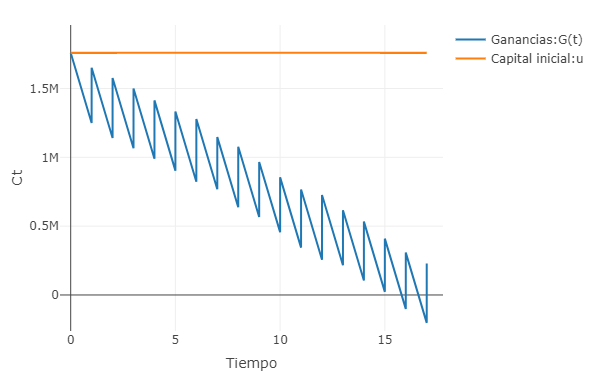
\includegraphics{trayectoria3pdf.png}

}

\caption{\label{fig-fig-trayectoria3pdf}}

\end{figure}%

La evolución del proceso de pérdidas en el modelo modificado de
Cramér-Lundberg proporciona una herramienta más precisa y adaptable para
predecir y contrarrestar los impactos financieros negativos de la
empresa.

Se incorpora un factor adicional y ajuste que mejoran la simulación del
modelo, mediante la modificación del parámetro \(c\), reduciendo un
\(17\%\) presentándose así los resultados siguientes mediante el
siguiente código.

\begin{Shaded}
\begin{Highlighting}[]
\FunctionTok{library}\NormalTok{(dplyr) }\CommentTok{\# libreria para poder renombrar }
\CommentTok{\# las cabeceras de los dataframes}

\CommentTok{\#Parametros}
\FunctionTok{set.seed}\NormalTok{(}\DecValTok{13}\NormalTok{) }\CommentTok{\#semilla fija}
\NormalTok{u }\OtherTok{=} \DecValTok{1759629} \CommentTok{\#surplus(capital inicial de salvamento)}
\CommentTok{\#Es un estimado a partir de la media de las ganancias por semana, }
\CommentTok{\#multiplicado por 10/3, }
\CommentTok{\#siendo una proporción para evitar la ruina}
\CommentTok{\# u (sum(medias))*(10/3)}
\NormalTok{c }\OtherTok{=}\NormalTok{ (}\FloatTok{0.29}\SpecialCharTok{*}\NormalTok{u)}\SpecialCharTok{*}\NormalTok{(}\FloatTok{0.83}\NormalTok{) }\CommentTok{\#prima de pago cada timepo t. c=0.5*u}
\NormalTok{lambda\_Nt }\OtherTok{=} \FloatTok{0.5}
\CommentTok{\#lambda\_Xi = 3}
\NormalTok{t\_final }\OtherTok{=} \DecValTok{14}
\CommentTok{\# S(t) = \textbackslash{}sum\_\{i=1\}\^{}\{N(t)\}X\_i}
\CommentTok{\#donde N(t)\textasciitilde{} Poisson (lambda*t)}
\CommentTok{\# X\_i \textasciitilde{} exponencial (lambda\_Xi)}
\CommentTok{\#CL = REPRESENTA EL MODELO DE CRAMER LUNDBERG}
\CommentTok{\#Simulación de trayectoria de CL\_t, cuando t \textless{} t\_final.}
\NormalTok{trayectoria\_CLt\_post\_pandemia }\OtherTok{\textless{}{-}} \ControlFlowTok{function}\NormalTok{(u, c, lambda\_Nt, t\_final)}
\NormalTok{\{}
\NormalTok{  tiempo }\OtherTok{\textless{}{-}} \FunctionTok{c}\NormalTok{(}\DecValTok{0}\NormalTok{)}
\NormalTok{  Cramer\_trayectoria }\OtherTok{\textless{}{-}} \FunctionTok{c}\NormalTok{(u)}
  \ControlFlowTok{while}\NormalTok{(tiempo[}\FunctionTok{length}\NormalTok{(tiempo)] }\SpecialCharTok{\textless{}}\NormalTok{ t\_final)}
\NormalTok{  \{}
\NormalTok{    tiempo\_llegada }\OtherTok{\textless{}{-}}\NormalTok{ (}\DecValTok{1}\NormalTok{)}\CommentTok{\#rexp(1, rate = lambda\_Nt)}
    
\NormalTok{    Y\_i }\OtherTok{\textless{}{-}}\NormalTok{  (}\FunctionTok{rnorm}\NormalTok{(}\DecValTok{1}\NormalTok{, }\AttributeTok{mean =} \FloatTok{101919.050}\NormalTok{ , }\AttributeTok{sd =} \FloatTok{10877.075}\NormalTok{) }\SpecialCharTok{+} 
            \FunctionTok{rnorm}\NormalTok{(}\DecValTok{1}\NormalTok{, }\AttributeTok{mean =}  \FloatTok{39841.721}\NormalTok{ , }\AttributeTok{sd=} \FloatTok{7873.446}\NormalTok{) }\SpecialCharTok{+}  
            \FunctionTok{rnorm}\NormalTok{(}\DecValTok{1}\NormalTok{, }\AttributeTok{mean =}   \FloatTok{41751.747}\NormalTok{, }\AttributeTok{sd =} \FloatTok{5687.030}\NormalTok{) }\SpecialCharTok{+} 
            \FunctionTok{rnorm}\NormalTok{(}\DecValTok{1}\NormalTok{, }\AttributeTok{mean =}   \FloatTok{43243.143}\NormalTok{, }\AttributeTok{sd =} \FloatTok{10517.841}\NormalTok{) }\SpecialCharTok{+} 
            \FunctionTok{rnorm}\NormalTok{(}\DecValTok{1}\NormalTok{, }\AttributeTok{mean =} \FloatTok{43010.307}\NormalTok{  , }\AttributeTok{sd =} \FloatTok{7741.889}\NormalTok{) }\SpecialCharTok{+} 
            \FunctionTok{rnorm}\NormalTok{(}\DecValTok{1}\NormalTok{, }\AttributeTok{mean =} \FloatTok{61191.300}\NormalTok{  , }\AttributeTok{sd =} \FloatTok{7202.989}\NormalTok{) }\SpecialCharTok{+} 
            \FunctionTok{rnorm}\NormalTok{(}\DecValTok{1}\NormalTok{, }\AttributeTok{mean =}  \FloatTok{85684.058}\NormalTok{ , }\AttributeTok{sd =} \FloatTok{8371.359}\NormalTok{ )) }
\NormalTok{    tiempo }\OtherTok{\textless{}{-}} \FunctionTok{c}\NormalTok{(tiempo, tiempo[}\FunctionTok{length}\NormalTok{(tiempo)] }\SpecialCharTok{+} 
\NormalTok{                tiempo\_llegada,tiempo[}\FunctionTok{length}\NormalTok{(tiempo)] }\SpecialCharTok{+} 
\NormalTok{                tiempo\_llegada ) }
\NormalTok{    Cramer\_trayectoria }\OtherTok{\textless{}{-}} \FunctionTok{c}\NormalTok{(Cramer\_trayectoria,}
\NormalTok{                    Cramer\_trayectoria[}\FunctionTok{length}\NormalTok{(Cramer\_trayectoria)]}\SpecialCharTok{{-}}
\NormalTok{                          c}\SpecialCharTok{*}\NormalTok{tiempo\_llegada, }
\NormalTok{                    Cramer\_trayectoria[}\FunctionTok{length}\NormalTok{(Cramer\_trayectoria)]}\SpecialCharTok{{-}} 
\NormalTok{                            c}\SpecialCharTok{*}\NormalTok{tiempo\_llegada }\SpecialCharTok{+}\NormalTok{ Y\_i )}
\NormalTok{  \}}
\NormalTok{  df\_post\_pandemia }\OtherTok{\textless{}{-}} \FunctionTok{data.frame}\NormalTok{(tiempo, Cramer\_trayectoria)}
\NormalTok{  df\_trayectoria\_post\_pandemia }\OtherTok{\textless{}{-}} \FunctionTok{data.frame}\NormalTok{(df\_post\_pandemia}\SpecialCharTok{\%\textgreater{}\%} 
                                          \FunctionTok{rename}\NormalTok{(}\AttributeTok{Tiempo =}\NormalTok{ tiempo, }
                                          \AttributeTok{Ct =}\NormalTok{ Cramer\_trayectoria))}
  \FunctionTok{return}\NormalTok{(df\_trayectoria\_post\_pandemia)}
\NormalTok{\}}
\NormalTok{trayectoria\_post\_pandemia }\OtherTok{\textless{}{-}} \FunctionTok{trayectoria\_CLt\_post\_pandemia}\NormalTok{(u,c,}
\NormalTok{                                            lambda\_Nt, t\_final )}


\FunctionTok{library}\NormalTok{(plotly)}
\CommentTok{\#plot(trayectoria$Tiempo, trayectoria$Ct, type= "l")}
\NormalTok{fig\_tr4 }\OtherTok{\textless{}{-}} \FunctionTok{plot\_ly}\NormalTok{(trayectoria\_post\_pandemia, }\AttributeTok{x =} \SpecialCharTok{\textasciitilde{}}\NormalTok{Tiempo, }
                   \AttributeTok{y =} \SpecialCharTok{\textasciitilde{}}\NormalTok{Ct, }
         \AttributeTok{name =} \StringTok{"Ganancias: G(t)"}\NormalTok{,}
         \AttributeTok{type =} \StringTok{"scatter"}\NormalTok{, }\AttributeTok{mode =} \StringTok{"lines"}\NormalTok{)}

\NormalTok{fig\_tr4 }\OtherTok{\textless{}{-}}\NormalTok{ fig\_tr4 }\SpecialCharTok{\%\textgreater{}\%} \FunctionTok{add\_trace}\NormalTok{(}\AttributeTok{x =} \SpecialCharTok{\textasciitilde{}}\NormalTok{Tiempo, }\AttributeTok{y =}\NormalTok{ u,}
        \AttributeTok{name =} \StringTok{"Capital inicial: u"}\NormalTok{, }
        \AttributeTok{type =} \StringTok{"scatter"}\NormalTok{, }\AttributeTok{mode =} \StringTok{"lines"}\NormalTok{)}
\NormalTok{fig\_tr4}
\end{Highlighting}
\end{Shaded}

\begin{figure}[H]

{\centering 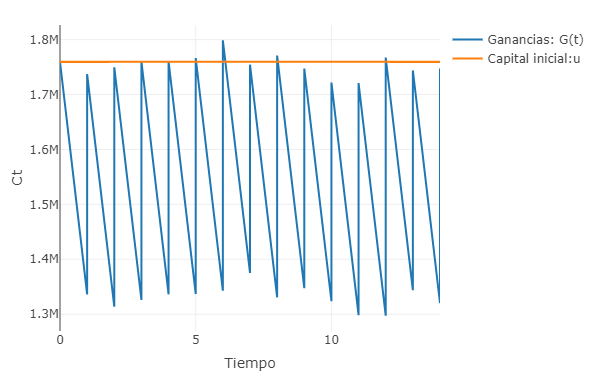
\includegraphics{trayectoria4pdf.png}

}

\caption{Trayectoria del proceso de pérdidas generadas por el modelo de
Cramér Lundberg después de la pandemia con una reducción de los costos
al 17\%.}

\end{figure}%

\subsubsection{Probabilidad de ruina}\label{probabilidad-de-ruina-1}

Al igual que para el caso con los datos antes de la pandemia se analizó
la semana en el que \(G(t)\leq u\) y cuando \(G(t)\leq0\), haciendo la
comparación con la tasa de interés de \(0.8\) anual en una cuenta de
ahorro para una inversión del capital inicial \(u\), para este periodo
tomamos \(t = 14\), es decir los datos registrados hasta las \(14\)
semanas después de pandemia donde la tasa es de \(0.0233\)

El código para calcular la probabilidad de las ganancias finales bajas
es el siguiente:

\begin{Shaded}
\begin{Highlighting}[]
\FunctionTok{library}\NormalTok{(dplyr) }\CommentTok{\# librería para poder renombrar las }
\CommentTok{\# cabeceras de los dataframes}

\CommentTok{\#Parámetros}
\FunctionTok{set.seed}\NormalTok{(}\DecValTok{13}\NormalTok{) }\CommentTok{\#semilla fija}
\NormalTok{u }\OtherTok{=} \DecValTok{1759629} \CommentTok{\#surplus(capital inicial de salvamento)}
\CommentTok{\#Es un estimado a partir de la media de las ganancias por semana, }
\CommentTok{\#multiplicado por 10/3, }
\CommentTok{\#siendo una proporción para evitar la ruina}
\CommentTok{\# u (sum(medias))*(10/3)}
\NormalTok{c }\OtherTok{=} \FloatTok{0.29}\SpecialCharTok{*}\NormalTok{u }\CommentTok{\#prima de pago cada timepo t. c=0.5*u}
\NormalTok{lambda\_Nt }\OtherTok{=} \FloatTok{0.5}
\CommentTok{\#lambda\_Xi = 3}
\NormalTok{t\_final }\OtherTok{=} \DecValTok{14}
\NormalTok{mu }\OtherTok{=} \DecValTok{1} \CommentTok{\#tiempos entrellegadas constantes}
\CommentTok{\# S(t) = \textbackslash{}sum\_\{i=1\}\^{}\{N(t)\}X\_i}
\CommentTok{\#donde N(t)\textasciitilde{} Poisson (lambda*t)}
\CommentTok{\# X\_i \textasciitilde{} exponencial (lambda\_Xi)}
\CommentTok{\#CL = REPRESENTA EL MODELO DE CRAMER LUNDBERG}
\CommentTok{\#Simulación de trayectoria de CL\_t, cuando t \textless{} t\_final.}
\NormalTok{trayectoria\_CLt\_post\_pandemia }\OtherTok{\textless{}{-}} \ControlFlowTok{function}\NormalTok{(u, c, lambda\_Nt, t\_final)}
\NormalTok{\{}
\NormalTok{  tiempo }\OtherTok{\textless{}{-}} \FunctionTok{c}\NormalTok{(}\DecValTok{0}\NormalTok{)}
\NormalTok{  Cramer\_trayectoria }\OtherTok{\textless{}{-}} \FunctionTok{c}\NormalTok{(u)}
  \ControlFlowTok{while}\NormalTok{(tiempo[}\FunctionTok{length}\NormalTok{(tiempo)] }\SpecialCharTok{\textless{}}\NormalTok{ t\_final)}
\NormalTok{  \{}
    \CommentTok{\#tiempo\_llegada \textless{}{-} rexp(1, rate = lambda\_Nt)}
\NormalTok{    tiempo\_llegada }\OtherTok{\textless{}{-}}\NormalTok{ (}\DecValTok{1}\NormalTok{) }
\CommentTok{\#Suponiendo los tiempos entrellegadas constantes \textbackslash{}mu = 1}
\NormalTok{    Y\_i }\OtherTok{\textless{}{-}}\NormalTok{  (}\FunctionTok{rnorm}\NormalTok{(}\DecValTok{1}\NormalTok{, }\AttributeTok{mean =} \FloatTok{101919.050}\NormalTok{ , }\AttributeTok{sd =} \FloatTok{10877.075}\NormalTok{   ) }
              \SpecialCharTok{+} \FunctionTok{rnorm}\NormalTok{(}\DecValTok{1}\NormalTok{, }\AttributeTok{mean =}  \FloatTok{39841.721}\NormalTok{ , }\AttributeTok{sd=} \FloatTok{7873.446}\NormalTok{  ) }
              \SpecialCharTok{+} \FunctionTok{rnorm}\NormalTok{(}\DecValTok{1}\NormalTok{, }\AttributeTok{mean =}   \FloatTok{41751.747}\NormalTok{, }\AttributeTok{sd =} \FloatTok{5687.030}\NormalTok{ ) }
              \SpecialCharTok{+} \FunctionTok{rnorm}\NormalTok{(}\DecValTok{1}\NormalTok{, }\AttributeTok{mean =}   \FloatTok{43243.143}\NormalTok{, }\AttributeTok{sd =} \FloatTok{10517.841}\NormalTok{) }
              \SpecialCharTok{+} \FunctionTok{rnorm}\NormalTok{(}\DecValTok{1}\NormalTok{, }\AttributeTok{mean =} \FloatTok{43010.307}\NormalTok{  , }\AttributeTok{sd =} \FloatTok{7741.889}\NormalTok{ ) }
              \SpecialCharTok{+} \FunctionTok{rnorm}\NormalTok{(}\DecValTok{1}\NormalTok{, }\AttributeTok{mean =} \FloatTok{61191.300}\NormalTok{  , }\AttributeTok{sd =} \FloatTok{7202.989}\NormalTok{ ) }
              \SpecialCharTok{+} \FunctionTok{rnorm}\NormalTok{(}\DecValTok{1}\NormalTok{, }\AttributeTok{mean =}  \FloatTok{85684.058}\NormalTok{ , }\AttributeTok{sd =} \FloatTok{8371.359}\NormalTok{)) }
\NormalTok{    tiempo }\OtherTok{\textless{}{-}} \FunctionTok{c}\NormalTok{(tiempo, tiempo[}\FunctionTok{length}\NormalTok{(tiempo)] }\SpecialCharTok{+} 
\NormalTok{                  tiempo\_llegada,tiempo[}\FunctionTok{length}\NormalTok{(tiempo)]}\SpecialCharTok{+} 
\NormalTok{                  tiempo\_llegada) }
\NormalTok{    Cramer\_trayectoria }\OtherTok{\textless{}{-}} \FunctionTok{c}\NormalTok{(Cramer\_trayectoria,}
\NormalTok{    Cramer\_trayectoria[}\FunctionTok{length}\NormalTok{(Cramer\_trayectoria)] }\SpecialCharTok{{-}} 
\NormalTok{      c}\SpecialCharTok{*}\NormalTok{tiempo\_llegada, }
\NormalTok{    Cramer\_trayectoria[}\FunctionTok{length}\NormalTok{(Cramer\_trayectoria)]}\SpecialCharTok{{-}} 
\NormalTok{      c}\SpecialCharTok{*}\NormalTok{tiempo\_llegada }\SpecialCharTok{+}\NormalTok{  Y\_i )}
    \ControlFlowTok{if}\NormalTok{(Cramer\_trayectoria[}\FunctionTok{length}\NormalTok{(Cramer\_trayectoria)] }\SpecialCharTok{\textless{}} \DecValTok{0}\NormalTok{)\{}
\NormalTok{      ruina }\OtherTok{=} \DecValTok{1}
\NormalTok{    \}}
    \ControlFlowTok{else}\NormalTok{\{}
\NormalTok{      ruina }\OtherTok{=} \DecValTok{0}
\NormalTok{    \}}
\NormalTok{  \}}
\CommentTok{\# 1.08*u es la ganancia inferior a la de un tasa de }
\CommentTok{\# un título financiero  para el año 2018}
  
  \ControlFlowTok{if}\NormalTok{(Cramer\_trayectoria[}\FunctionTok{length}\NormalTok{(Cramer\_trayectoria)] }\SpecialCharTok{\textless{}}\NormalTok{ (}\DecValTok{1} \SpecialCharTok{+}\NormalTok{ (}\DecValTok{14}\SpecialCharTok{*}\FloatTok{0.08}\NormalTok{)}\SpecialCharTok{/}\DecValTok{48}\NormalTok{)}\SpecialCharTok{*}\NormalTok{u) \{}
\NormalTok{    ganancia\_no\_deseada }\OtherTok{=} \DecValTok{1}
    
\NormalTok{  \} }
  \ControlFlowTok{else}\NormalTok{\{}
\NormalTok{    ganancia\_no\_deseada }\OtherTok{=} \DecValTok{0}
\NormalTok{  \}}
\NormalTok{  df\_post\_pandemia }\OtherTok{\textless{}{-}} \FunctionTok{data.frame}\NormalTok{(tiempo, Cramer\_trayectoria)}
\NormalTok{  df\_trayectoria\_post\_pandemia }\OtherTok{\textless{}{-}} \FunctionTok{data.frame}\NormalTok{(df\_post\_pandemia}\SpecialCharTok{\%\textgreater{}\%} 
                                  \FunctionTok{rename}\NormalTok{(}\AttributeTok{Tiempo =}\NormalTok{ tiempo,}
                                         \AttributeTok{Ct =}\NormalTok{ Cramer\_trayectoria))}
\NormalTok{  salida }\OtherTok{\textless{}{-}} \FunctionTok{c}\NormalTok{(ruina, ganancia\_no\_deseada)}
  \FunctionTok{return}\NormalTok{(salida)}
  
\NormalTok{\}}
\NormalTok{trayectoria\_post\_pandemia }\OtherTok{\textless{}{-}} \FunctionTok{trayectoria\_CLt\_post\_pandemia}\NormalTok{(u,c,}
\NormalTok{                                            lambda\_Nt, t\_final )}
\CommentTok{\#Método de monte carlo para estimar la probabilidad de ruina}
\NormalTok{n\_replicaciones }\OtherTok{=} \DecValTok{100}
\NormalTok{r\_baja\_ganancia\_post\_pandemia }\OtherTok{\textless{}{-}} \FunctionTok{replicate}\NormalTok{(n\_replicaciones,}
                          \FunctionTok{trayectoria\_CLt\_post\_pandemia}\NormalTok{(u, c, }
\NormalTok{                                         lambda\_Nt, t\_final)[}\DecValTok{2}\NormalTok{])}
\NormalTok{r\_baja\_ganancia\_post\_pandemia }
\NormalTok{prob\_baja\_ganancia\_post\_pandemia }\OtherTok{\textless{}{-}} \FunctionTok{sum}\NormalTok{(r\_baja\_ganancia\_post\_pandemia }\SpecialCharTok{\textgreater{}}\DecValTok{0}\NormalTok{)}\SpecialCharTok{/}
\NormalTok{n\_replicaciones}
\NormalTok{prob\_baja\_ganancia\_post\_pandemia}
\end{Highlighting}
\end{Shaded}

Claramente la probabilidad de las ganancias bajas de la evolución de
\(G(t)\) después de la pandemia sea \(1\), pues como se muestra en la
Figura~\ref{fig-fig-trayectoria2pdf} todas las ventas registradas están
por debajo del capital inicial

\begin{verbatim}
[1] 1
\end{verbatim}

El código para calcular la probabilidad de las ganancias finales bajas
durante las \(17\) semanas es el siguiente:

\begin{Shaded}
\begin{Highlighting}[]
\FunctionTok{library}\NormalTok{(dplyr) }\CommentTok{\# libreria para poder renombrar }
\CommentTok{\#las cabeceras de los dataframes}

\CommentTok{\#Parametros}
\FunctionTok{set.seed}\NormalTok{(}\DecValTok{13}\NormalTok{) }\CommentTok{\#semilla fija}
\NormalTok{u }\OtherTok{=} \DecValTok{1759629} \CommentTok{\#surplus(capital inicial de salvamento)}
\CommentTok{\#Es un estimado a partir de la media de las ganancias por semana, }
\CommentTok{\#multiplicado por 10/3, }
\CommentTok{\#siendo una proporción para evitar la ruina}
\CommentTok{\# u (sum(medias))*(10/3)}
\NormalTok{c }\OtherTok{=} \FloatTok{0.29}\SpecialCharTok{*}\NormalTok{u }\CommentTok{\#prima de pago cada timepo t. c=0.5*u}
\NormalTok{lambda\_Nt }\OtherTok{=} \FloatTok{0.5}
\CommentTok{\#lambda\_Xi = 3}
\NormalTok{t\_final }\OtherTok{=} \DecValTok{17}
\NormalTok{mu }\OtherTok{=} \DecValTok{1} \CommentTok{\#tiempos entrellegadas constantes}
\CommentTok{\#df\_media \textless{}{-} data.frame(df\_media\%\textgreater{}\% rename(tiempos = Tiempo ,}
\CommentTok{\#media\_trayectoria = cramer\_media)}
\CommentTok{\# S(t) = \textbackslash{}sum\_\{i=1\}\^{}\{N(t)\}X\_i}
\CommentTok{\#donde N(t)\textasciitilde{} Poisson (lambda*t)}
\CommentTok{\# X\_i \textasciitilde{} exponencial (lambda\_Xi)}
\CommentTok{\#CL = REPRESENTA EL MODELO DE CRAMER LUNDBERG}
\CommentTok{\#Simulación de trayectoria de CL\_t, cuando t \textless{} t\_final.}
\NormalTok{trayectoria\_CLt\_post\_pandemia }\OtherTok{\textless{}{-}} \ControlFlowTok{function}\NormalTok{(u, c, lambda\_Nt, t\_final)}
\NormalTok{\{}
\NormalTok{  tiempo }\OtherTok{\textless{}{-}} \FunctionTok{c}\NormalTok{(}\DecValTok{0}\NormalTok{)}
\NormalTok{  Cramer\_trayectoria }\OtherTok{\textless{}{-}} \FunctionTok{c}\NormalTok{(u)}
  \ControlFlowTok{while}\NormalTok{(tiempo[}\FunctionTok{length}\NormalTok{(tiempo)] }\SpecialCharTok{\textless{}}\NormalTok{ t\_final)}
\NormalTok{  \{}
    \CommentTok{\#tiempo\_llegada \textless{}{-} rexp(1, rate = lambda\_Nt)}
\NormalTok{    tiempo\_llegada }\OtherTok{\textless{}{-}}\NormalTok{ (}\DecValTok{1}\NormalTok{) }
\CommentTok{\#Suponiendo los tiempos entrellegadas constantes \textbackslash{}mu = 1}
\NormalTok{    Y\_i }\OtherTok{\textless{}{-}}\NormalTok{  (}\FunctionTok{rnorm}\NormalTok{(}\DecValTok{1}\NormalTok{, }\AttributeTok{mean =} \FloatTok{101919.050}\NormalTok{ , }\AttributeTok{sd =} \FloatTok{10877.075}\NormalTok{)}\SpecialCharTok{+} 
              \FunctionTok{rnorm}\NormalTok{(}\DecValTok{1}\NormalTok{, }\AttributeTok{mean =}  \FloatTok{39841.721}\NormalTok{ , }\AttributeTok{sd=} \FloatTok{7873.446}\NormalTok{) }\SpecialCharTok{+} 
              \FunctionTok{rnorm}\NormalTok{(}\DecValTok{1}\NormalTok{, }\AttributeTok{mean =}   \FloatTok{41751.747}\NormalTok{, }\AttributeTok{sd =} \FloatTok{5687.030}\NormalTok{)}\SpecialCharTok{+} 
              \FunctionTok{rnorm}\NormalTok{(}\DecValTok{1}\NormalTok{, }\AttributeTok{mean =}   \FloatTok{43243.143}\NormalTok{, }\AttributeTok{sd =} \FloatTok{10517.841}\NormalTok{)}\SpecialCharTok{+} 
              \FunctionTok{rnorm}\NormalTok{(}\DecValTok{1}\NormalTok{, }\AttributeTok{mean =} \FloatTok{43010.307}\NormalTok{  , }\AttributeTok{sd =} \FloatTok{7741.889}\NormalTok{)}\SpecialCharTok{+} 
              \FunctionTok{rnorm}\NormalTok{(}\DecValTok{1}\NormalTok{, }\AttributeTok{mean =} \FloatTok{61191.300}\NormalTok{  , }\AttributeTok{sd =} \FloatTok{7202.989}\NormalTok{)}\SpecialCharTok{+} 
              \FunctionTok{rnorm}\NormalTok{(}\DecValTok{1}\NormalTok{, }\AttributeTok{mean =}  \FloatTok{85684.058}\NormalTok{ , }\AttributeTok{sd =} \FloatTok{8371.359}\NormalTok{ )) }
\NormalTok{    tiempo }\OtherTok{\textless{}{-}} \FunctionTok{c}\NormalTok{(tiempo, tiempo[}\FunctionTok{length}\NormalTok{(tiempo)]}\SpecialCharTok{+} 
\NormalTok{                  tiempo\_llegada,tiempo[}\FunctionTok{length}\NormalTok{(tiempo)]}\SpecialCharTok{+} 
\NormalTok{                  tiempo\_llegada ) }
\NormalTok{    Cramer\_trayectoria }\OtherTok{\textless{}{-}} \FunctionTok{c}\NormalTok{(Cramer\_trayectoria,}
\NormalTok{                      Cramer\_trayectoria[}\FunctionTok{length}\NormalTok{(Cramer\_trayectoria)]}\SpecialCharTok{{-}}
\NormalTok{                      c}\SpecialCharTok{*}\NormalTok{tiempo\_llegada, }
\NormalTok{                      Cramer\_trayectoria[}\FunctionTok{length}\NormalTok{(Cramer\_trayectoria)]}\SpecialCharTok{{-}} 
\NormalTok{                      c}\SpecialCharTok{*}\NormalTok{tiempo\_llegada }\SpecialCharTok{+}\NormalTok{  Y\_i )}
    \ControlFlowTok{if}\NormalTok{(Cramer\_trayectoria[}\FunctionTok{length}\NormalTok{(Cramer\_trayectoria)] }\SpecialCharTok{\textless{}} \DecValTok{0}\NormalTok{)\{}
\NormalTok{      ruina }\OtherTok{=} \DecValTok{1}
\NormalTok{    \}}
    \ControlFlowTok{else}\NormalTok{\{}
\NormalTok{      ruina }\OtherTok{=} \DecValTok{0}
\NormalTok{    \}}
\NormalTok{  \}}
\CommentTok{\# 1.08*u es la ganancia inferior a la de un tasa de }
\CommentTok{\# un título financieropara el año 2018}
  \ControlFlowTok{if}\NormalTok{(Cramer\_trayectoria[}\FunctionTok{length}\NormalTok{(Cramer\_trayectoria)] }\SpecialCharTok{\textless{}} \FloatTok{1.02833}\SpecialCharTok{*}\NormalTok{u) \{}
\NormalTok{    ganancia\_no\_deseada }\OtherTok{=} \DecValTok{1}
    
\NormalTok{  \} }
  \ControlFlowTok{else}\NormalTok{\{}
\NormalTok{    ganancia\_no\_deseada }\OtherTok{=} \DecValTok{0}
\NormalTok{  \}}
\NormalTok{  df\_post\_pandemia }\OtherTok{\textless{}{-}} \FunctionTok{data.frame}\NormalTok{(tiempo, Cramer\_trayectoria)}
\NormalTok{  df\_trayectoria\_post\_pandemia }\OtherTok{\textless{}{-}} \FunctionTok{data.frame}\NormalTok{(df\_post\_pandemia}\SpecialCharTok{\%\textgreater{}\%}
                                            \FunctionTok{rename}\NormalTok{(}\AttributeTok{Tiempo =}\NormalTok{ tiempo, }
                                            \AttributeTok{Ct =}\NormalTok{ Cramer\_trayectoria))}
\NormalTok{  salida }\OtherTok{\textless{}{-}} \FunctionTok{c}\NormalTok{(ruina, ganancia\_no\_deseada)}
  \FunctionTok{return}\NormalTok{(salida)}
  
\NormalTok{\}}
\NormalTok{trayectoria\_post\_pandemia }\OtherTok{\textless{}{-}} \FunctionTok{trayectoria\_CLt\_post\_pandemia}\NormalTok{(u,c,}
\NormalTok{                                            lambda\_Nt, t\_final )}
\CommentTok{\#Método de monte carlo para estimar la probabilidad de ruina}
\NormalTok{n\_replicaciones }\OtherTok{=} \DecValTok{100}
\NormalTok{r\_baja\_ganancia\_post\_pandemia }\OtherTok{\textless{}{-}} \FunctionTok{replicate}\NormalTok{(n\_replicaciones, }
          \FunctionTok{trayectoria\_CLt\_post\_pandemia}\NormalTok{(u, c, lambda\_Nt, t\_final)[}\DecValTok{2}\NormalTok{])}
\CommentTok{\#r\_baja\_ganancia\_post\_pandemia }
\NormalTok{prob\_baja\_ganancia\_post\_pandemia }\OtherTok{\textless{}{-}} \FunctionTok{sum}\NormalTok{(r\_baja\_ganancia\_post\_pandemia }\SpecialCharTok{\textgreater{}}\DecValTok{0}\NormalTok{)}\SpecialCharTok{/}
\NormalTok{n\_replicaciones}
\NormalTok{prob\_baja\_ganancia\_post\_pandemia}
\end{Highlighting}
\end{Shaded}

\begin{verbatim}
[1] 1
\end{verbatim}

El código para calcular la probabilidad de ruina es el siguiente:

\begin{Shaded}
\begin{Highlighting}[]
\FunctionTok{library}\NormalTok{(dplyr) }\CommentTok{\# libreria para poder renombrar }
\CommentTok{\#las cabeceras de los dataframes}

\CommentTok{\#Parametros}
\FunctionTok{set.seed}\NormalTok{(}\DecValTok{13}\NormalTok{) }\CommentTok{\#semilla fija}
\NormalTok{u }\OtherTok{=} \DecValTok{1759629} \CommentTok{\#surplus(capital inicial de salvamento)}
\CommentTok{\#Es un estimado a partir de la media de las ganancias por semana, }
\CommentTok{\#multiplicado por 10/3, }
\CommentTok{\#siendo una proporción para evitar la ruina}
\CommentTok{\# u (sum(medias))*(10/3)}
\NormalTok{c }\OtherTok{=} \FloatTok{0.29}\SpecialCharTok{*}\NormalTok{u }\CommentTok{\#prima de pago cada timepo t. c=0.5*u}
\NormalTok{lambda\_Nt }\OtherTok{=} \FloatTok{0.5}
\CommentTok{\#lambda\_Xi = 3}
\NormalTok{t\_final }\OtherTok{=} \DecValTok{14}
\NormalTok{mu }\OtherTok{=} \DecValTok{1} \CommentTok{\#tiempos entrellegadas constantes}
\CommentTok{\#df\_media \textless{}{-} data.frame(df\_media\%\textgreater{}\% rename(tiempos = Tiempo , }
\CommentTok{\#media\_trayectoria = cramer\_media)}
\CommentTok{\# S(t) = \textbackslash{}sum\_\{i=1\}\^{}\{N(t)\}X\_i}
\CommentTok{\#donde N(t)\textasciitilde{} Poisson (lambda*t)}
\CommentTok{\# X\_i \textasciitilde{} exponencial (lambda\_Xi)}
\CommentTok{\#CL = REPRESENTA EL MODELO DE CRAMER LUNDBERG}
\CommentTok{\#Simulación de trayectoria de CL\_t, cuando t \textless{} t\_final.}
\NormalTok{trayectoria\_CLt\_post\_pandemia }\OtherTok{\textless{}{-}} \ControlFlowTok{function}\NormalTok{(u, c, lambda\_Nt, t\_final)}
\NormalTok{\{}
\NormalTok{  tiempo }\OtherTok{\textless{}{-}} \FunctionTok{c}\NormalTok{(}\DecValTok{0}\NormalTok{)}
\NormalTok{  Cramer\_trayectoria }\OtherTok{\textless{}{-}} \FunctionTok{c}\NormalTok{(u)}
  \ControlFlowTok{while}\NormalTok{(tiempo[}\FunctionTok{length}\NormalTok{(tiempo)] }\SpecialCharTok{\textless{}}\NormalTok{ t\_final)}
\NormalTok{  \{}
    \CommentTok{\#tiempo\_llegada \textless{}{-} rexp(1, rate = lambda\_Nt)}
\NormalTok{    tiempo\_llegada }\OtherTok{\textless{}{-}}\NormalTok{ (}\DecValTok{1}\NormalTok{) }
\CommentTok{\#Suponiendo los tiempos entrellegadas constantes \textbackslash{}mu = 1}
\NormalTok{    Y\_i }\OtherTok{\textless{}{-}}\NormalTok{  (}\FunctionTok{rnorm}\NormalTok{(}\DecValTok{1}\NormalTok{, }\AttributeTok{mean =} \FloatTok{101919.050}\NormalTok{ , }\AttributeTok{sd =} \FloatTok{10877.075}\NormalTok{)  }\SpecialCharTok{+}
               \FunctionTok{rnorm}\NormalTok{(}\DecValTok{1}\NormalTok{, }\AttributeTok{mean =}  \FloatTok{39841.721}\NormalTok{ , }\AttributeTok{sd=} \FloatTok{7873.446}\NormalTok{ ) }\SpecialCharTok{+} 
               \FunctionTok{rnorm}\NormalTok{(}\DecValTok{1}\NormalTok{, }\AttributeTok{mean =}   \FloatTok{41751.747}\NormalTok{, }\AttributeTok{sd =} \FloatTok{5687.030}\NormalTok{) }\SpecialCharTok{+} 
               \FunctionTok{rnorm}\NormalTok{(}\DecValTok{1}\NormalTok{, }\AttributeTok{mean =}   \FloatTok{43243.143}\NormalTok{, }\AttributeTok{sd =} \FloatTok{10517.841}\NormalTok{)}\SpecialCharTok{+} 
               \FunctionTok{rnorm}\NormalTok{(}\DecValTok{1}\NormalTok{, }\AttributeTok{mean =} \FloatTok{43010.307}\NormalTok{  , }\AttributeTok{sd =} \FloatTok{7741.889}\NormalTok{ )}\SpecialCharTok{+}
               \FunctionTok{rnorm}\NormalTok{(}\DecValTok{1}\NormalTok{, }\AttributeTok{mean =} \FloatTok{61191.300}\NormalTok{  , }\AttributeTok{sd =} \FloatTok{7202.989}\NormalTok{) }\SpecialCharTok{+}
               \FunctionTok{rnorm}\NormalTok{(}\DecValTok{1}\NormalTok{, }\AttributeTok{mean =}  \FloatTok{85684.058}\NormalTok{ , }\AttributeTok{sd =} \FloatTok{8371.359}\NormalTok{ )) }
\NormalTok{    tiempo }\OtherTok{\textless{}{-}} \FunctionTok{c}\NormalTok{(tiempo, tiempo[}\FunctionTok{length}\NormalTok{(tiempo)] }\SpecialCharTok{+}
\NormalTok{                  tiempo\_llegada,tiempo[}\FunctionTok{length}\NormalTok{(tiempo)] }\SpecialCharTok{+} 
\NormalTok{                  tiempo\_llegada ) }
\NormalTok{    Cramer\_trayectoria }\OtherTok{\textless{}{-}} \FunctionTok{c}\NormalTok{(Cramer\_trayectoria,}
\NormalTok{                       Cramer\_trayectoria[}\FunctionTok{length}\NormalTok{(Cramer\_trayectoria)]}\SpecialCharTok{{-}}
\NormalTok{                          c}\SpecialCharTok{*}\NormalTok{tiempo\_llegada, }
\NormalTok{                       Cramer\_trayectoria[}\FunctionTok{length}\NormalTok{(Cramer\_trayectoria)]}\SpecialCharTok{{-}}
\NormalTok{                         c}\SpecialCharTok{*}\NormalTok{tiempo\_llegada }\SpecialCharTok{+}\NormalTok{  Y\_i )}
    \ControlFlowTok{if}\NormalTok{(Cramer\_trayectoria[}\FunctionTok{length}\NormalTok{(Cramer\_trayectoria)] }\SpecialCharTok{\textless{}} \DecValTok{0}\NormalTok{)\{}
\NormalTok{      ruina }\OtherTok{=} \DecValTok{1}
\NormalTok{    \}}
    \ControlFlowTok{else}\NormalTok{\{}
\NormalTok{      ruina }\OtherTok{=} \DecValTok{0}
\NormalTok{    \}}
\NormalTok{  \}}
\CommentTok{\# 1.08*u es la ganancia inferior a la de un tasa de }
\CommentTok{\# un título financiero para el año 2018}
  \ControlFlowTok{if}\NormalTok{(Cramer\_trayectoria[}\FunctionTok{length}\NormalTok{(Cramer\_trayectoria)] }\SpecialCharTok{\textless{}} \FloatTok{1.02333}\SpecialCharTok{*}\NormalTok{u) \{}
\NormalTok{    ganancia\_no\_deseada }\OtherTok{=} \DecValTok{1}
    
\NormalTok{  \} }
  \ControlFlowTok{else}\NormalTok{\{}
\NormalTok{    ganancia\_no\_deseada }\OtherTok{=} \DecValTok{0}
\NormalTok{  \}}
\NormalTok{  df\_post\_pandemia }\OtherTok{\textless{}{-}} \FunctionTok{data.frame}\NormalTok{(tiempo, Cramer\_trayectoria)}
\NormalTok{  df\_trayectoria\_post\_pandemia }\OtherTok{\textless{}{-}} \FunctionTok{data.frame}\NormalTok{(df\_post\_pandemia}\SpecialCharTok{\%\textgreater{}\%} 
                                  \FunctionTok{rename}\NormalTok{(}\AttributeTok{Tiempo =}\NormalTok{ tiempo, }
                                  \AttributeTok{Ct =}\NormalTok{ Cramer\_trayectoria))}
\NormalTok{  salida }\OtherTok{\textless{}{-}} \FunctionTok{c}\NormalTok{(ruina, ganancia\_no\_deseada)}
  \FunctionTok{return}\NormalTok{(salida)}
  
\NormalTok{\}}
\NormalTok{trayectoria\_post\_pandemia }\OtherTok{\textless{}{-}} \FunctionTok{trayectoria\_CLt\_post\_pandemia}\NormalTok{(u,c,}
\NormalTok{                                            lambda\_Nt, t\_final )}
\CommentTok{\#Método de monte carlo para estimar la probabilidad de ruina}
\NormalTok{n\_replicaciones }\OtherTok{=} \DecValTok{100}
\NormalTok{r\_ruina\_post\_pandemia }\OtherTok{\textless{}{-}} \FunctionTok{replicate}\NormalTok{(n\_replicaciones,}
          \FunctionTok{trayectoria\_CLt\_post\_pandemia}\NormalTok{(u, c, lambda\_Nt, t\_final)[}\DecValTok{1}\NormalTok{])}
\CommentTok{\#r\_ruina\_post\_pandemia}
\NormalTok{prob\_ruin\_post\_pandemia }\OtherTok{\textless{}{-}} \FunctionTok{sum}\NormalTok{(r\_ruina\_post\_pandemia}\SpecialCharTok{\textgreater{}}\DecValTok{0}\NormalTok{)}\SpecialCharTok{/}
\NormalTok{n\_replicaciones}
\NormalTok{prob\_ruin\_post\_pandemia}
\end{Highlighting}
\end{Shaded}

Lo que significa que a pesar de que las ganancias sean todas menores al
capital inicial, en todas la simulaciones, nunca se presenta una que sea
menor que cero.

\begin{verbatim}
[1] 0
\end{verbatim}

El código para calcular la probabilidad de ruina durante las \(17\)
semanas es el siguiente:

\begin{Shaded}
\begin{Highlighting}[]
\FunctionTok{library}\NormalTok{(dplyr) }\CommentTok{\# libreria para poder renombrar }
\CommentTok{\#las cabeceras de los dataframes}

\CommentTok{\#Parametros}
\FunctionTok{set.seed}\NormalTok{(}\DecValTok{13}\NormalTok{) }\CommentTok{\#semilla fija}
\NormalTok{u }\OtherTok{=} \DecValTok{1759629} \CommentTok{\#surplus(capital inicial de salvamento)}
\CommentTok{\#Es un estimado a partir de la media de las ganancias por semana, }
\CommentTok{\#multiplicado por 10/3, }
\CommentTok{\#siendo una proporción para evitar la ruina}
\CommentTok{\# u (sum(medias))*(10/3)}
\NormalTok{c }\OtherTok{=} \FloatTok{0.29}\SpecialCharTok{*}\NormalTok{u }\CommentTok{\#prima de pago cada timepo t. c=0.5*u}
\NormalTok{lambda\_Nt }\OtherTok{=} \FloatTok{0.5}
\CommentTok{\#lambda\_Xi = 3}
\NormalTok{t\_final }\OtherTok{=} \DecValTok{17}
\NormalTok{mu }\OtherTok{=} \DecValTok{1} \CommentTok{\#tiempos entrellegadas constantes}
\CommentTok{\#df\_media \textless{}{-} data.frame(df\_media\%\textgreater{}\% rename(tiempos = Tiempo , }
\CommentTok{\#media\_trayectoria = cramer\_media)}
\CommentTok{\# S(t) = \textbackslash{}sum\_\{i=1\}\^{}\{N(t)\}X\_i}
\CommentTok{\#donde N(t)\textasciitilde{} Poisson (lambda*t)}
\CommentTok{\# X\_i \textasciitilde{} exponencial (lambda\_Xi)}
\CommentTok{\#CL = REPRESENTA EL MODELO DE CRAMER LUNDBERG}
\CommentTok{\#Simulación de trayectoria de CL\_t, cuando t \textless{} t\_final.}
\NormalTok{trayectoria\_CLt\_post\_pandemia }\OtherTok{\textless{}{-}} \ControlFlowTok{function}\NormalTok{(u, c, lambda\_Nt, t\_final)}
\NormalTok{\{}
\NormalTok{  tiempo }\OtherTok{\textless{}{-}} \FunctionTok{c}\NormalTok{(}\DecValTok{0}\NormalTok{)}
\NormalTok{  Cramer\_trayectoria }\OtherTok{\textless{}{-}} \FunctionTok{c}\NormalTok{(u)}
  \ControlFlowTok{while}\NormalTok{(tiempo[}\FunctionTok{length}\NormalTok{(tiempo)] }\SpecialCharTok{\textless{}}\NormalTok{ t\_final)}
\NormalTok{  \{}
    \CommentTok{\#tiempo\_llegada \textless{}{-} rexp(1, rate = lambda\_Nt)}
\NormalTok{    tiempo\_llegada }\OtherTok{\textless{}{-}}\NormalTok{ (}\DecValTok{1}\NormalTok{) }
\CommentTok{\# Suponiendo los tiempos entrellegadas constantes \textbackslash{}mu = 1}
\NormalTok{    Y\_i }\OtherTok{\textless{}{-}}\NormalTok{  (}\FunctionTok{rnorm}\NormalTok{(}\DecValTok{1}\NormalTok{, }\AttributeTok{mean =} \FloatTok{101919.050}\NormalTok{ , }\AttributeTok{sd =} \FloatTok{10877.075}\NormalTok{)  }\SpecialCharTok{+} 
               \FunctionTok{rnorm}\NormalTok{(}\DecValTok{1}\NormalTok{, }\AttributeTok{mean =}  \FloatTok{39841.721}\NormalTok{ , }\AttributeTok{sd=} \FloatTok{7873.446}\NormalTok{)  }\SpecialCharTok{+}  
               \FunctionTok{rnorm}\NormalTok{(}\DecValTok{1}\NormalTok{, }\AttributeTok{mean =}   \FloatTok{41751.747}\NormalTok{, }\AttributeTok{sd =} \FloatTok{5687.030}\NormalTok{) }\SpecialCharTok{+} 
               \FunctionTok{rnorm}\NormalTok{(}\DecValTok{1}\NormalTok{, }\AttributeTok{mean =}   \FloatTok{43243.143}\NormalTok{, }\AttributeTok{sd =} \FloatTok{10517.841}\NormalTok{)}\SpecialCharTok{+} 
               \FunctionTok{rnorm}\NormalTok{(}\DecValTok{1}\NormalTok{, }\AttributeTok{mean =} \FloatTok{43010.307}\NormalTok{  , }\AttributeTok{sd =} \FloatTok{7741.889}\NormalTok{) }\SpecialCharTok{+} 
               \FunctionTok{rnorm}\NormalTok{(}\DecValTok{1}\NormalTok{, }\AttributeTok{mean =}  \FloatTok{85684.058}\NormalTok{ , }\AttributeTok{sd =} \FloatTok{8371.359}\NormalTok{)) }
\NormalTok{    tiempo }\OtherTok{\textless{}{-}} \FunctionTok{c}\NormalTok{(tiempo, tiempo[}\FunctionTok{length}\NormalTok{(tiempo)] }\SpecialCharTok{+} 
\NormalTok{                  tiempo\_llegada,tiempo[}\FunctionTok{length}\NormalTok{(tiempo)] }\SpecialCharTok{+} 
\NormalTok{                  tiempo\_llegada ) }
\NormalTok{    Cramer\_trayectoria }\OtherTok{\textless{}{-}} \FunctionTok{c}\NormalTok{(Cramer\_trayectoria,}
\NormalTok{                      Cramer\_trayectoria[}\FunctionTok{length}\NormalTok{(Cramer\_trayectoria)]}\SpecialCharTok{{-}}
\NormalTok{                      c}\SpecialCharTok{*}\NormalTok{tiempo\_llegada, }
\NormalTok{                      Cramer\_trayectoria[}\FunctionTok{length}\NormalTok{(Cramer\_trayectoria)]}\SpecialCharTok{{-}} 
\NormalTok{                      c}\SpecialCharTok{*}\NormalTok{tiempo\_llegada }\SpecialCharTok{+}\NormalTok{  Y\_i )}
    \ControlFlowTok{if}\NormalTok{(Cramer\_trayectoria[}\FunctionTok{length}\NormalTok{(Cramer\_trayectoria)] }\SpecialCharTok{\textless{}} \DecValTok{0}\NormalTok{)\{}
\NormalTok{      ruina }\OtherTok{=} \DecValTok{1}
\NormalTok{    \}}
    \ControlFlowTok{else}\NormalTok{\{}
\NormalTok{      ruina }\OtherTok{=} \DecValTok{0}
\NormalTok{    \}}
\NormalTok{  \}}
\CommentTok{\# 1.08*u es la ganancia inferior a la de }
\CommentTok{\# un tasa de un título financiero para el año 2018}
  \ControlFlowTok{if}\NormalTok{(Cramer\_trayectoria[}\FunctionTok{length}\NormalTok{(Cramer\_trayectoria)] }\SpecialCharTok{\textless{}} \FloatTok{1.02833}\SpecialCharTok{*}\NormalTok{u) \{}
\NormalTok{    ganancia\_no\_deseada }\OtherTok{=} \DecValTok{1}
    
\NormalTok{  \} }
  \ControlFlowTok{else}\NormalTok{\{}
\NormalTok{    ganancia\_no\_deseada }\OtherTok{=} \DecValTok{0}
\NormalTok{  \}}
\NormalTok{  df\_post\_pandemia }\OtherTok{\textless{}{-}} \FunctionTok{data.frame}\NormalTok{(tiempo, Cramer\_trayectoria)}
\NormalTok{  df\_trayectoria\_post\_pandemia }\OtherTok{\textless{}{-}} \FunctionTok{data.frame}\NormalTok{(df\_post\_pandemia}\SpecialCharTok{\%\textgreater{}\%} 
                                  \FunctionTok{rename}\NormalTok{(}\AttributeTok{Tiempo =}\NormalTok{ tiempo, }
                                         \AttributeTok{Ct =}\NormalTok{ Cramer\_trayectoria))}
\NormalTok{  salida }\OtherTok{\textless{}{-}} \FunctionTok{c}\NormalTok{(ruina, ganancia\_no\_deseada)}
  \FunctionTok{return}\NormalTok{(salida)}
  
\NormalTok{\}}
\NormalTok{trayectoria\_post\_pandemia }\OtherTok{\textless{}{-}} \FunctionTok{trayectoria\_CLt\_post\_pandemia}\NormalTok{(u,c,}
\NormalTok{                                            lambda\_Nt, t\_final )}
\CommentTok{\#Método de monte carlo para estimar la probabilidad de ruina}
\NormalTok{n\_replicaciones }\OtherTok{=} \DecValTok{100}
\NormalTok{r\_ruina\_post\_pandemia }\OtherTok{\textless{}{-}} \FunctionTok{replicate}\NormalTok{(n\_replicaciones,}
                          \FunctionTok{trayectoria\_CLt\_post\_pandemia}\NormalTok{(u, c, }
\NormalTok{                                          lambda\_Nt, t\_final)[}\DecValTok{1}\NormalTok{])}
\CommentTok{\#r\_ruina\_post\_pandemia}
\NormalTok{prob\_ruin\_post\_pandemia }\OtherTok{\textless{}{-}} \FunctionTok{sum}\NormalTok{(r\_ruina\_post\_pandemia}\SpecialCharTok{\textgreater{}}\DecValTok{0}\NormalTok{)}\SpecialCharTok{/}
\NormalTok{n\_replicaciones}
\NormalTok{prob\_ruin\_post\_pandemia}
\end{Highlighting}
\end{Shaded}

\begin{verbatim}
[1] 1
\end{verbatim}

\subsubsection{Análisis de
sensibilidad}\label{anuxe1lisis-de-sensibilidad-1}

Modificando los parámetros \(u\) y \(c\) para erl periodo pso-pandemia
del modelo modificado y estableciendo los rangos o valores posibles para
cada uno de los ciertos parámetros, se presenta el análisis de
sensibilidad durante las semanas registradas después de la pandemia que
fueron \(14\),. Se toman la mediana de las \(100\) simulaciones de la
ganancia final de la semana obtenida por el modelo, es decir la venta
registrada en la última semana de los datos registrados.

\begin{Shaded}
\begin{Highlighting}[]
\FunctionTok{library}\NormalTok{(dplyr) }\CommentTok{\# libreria para poder renombrar }
\CommentTok{\# las cabeceras de los dataframes}

\CommentTok{\#Parametros}
\FunctionTok{set.seed}\NormalTok{(}\DecValTok{13}\NormalTok{) }\CommentTok{\#semilla fija}
\NormalTok{u }\OtherTok{=} \DecValTok{1759629} \CommentTok{\#surplus(capital inicial de salvamento)}
\CommentTok{\#Es un estimado a partir de la media de las ganancias por semana, }
\CommentTok{\#multiplicado por 10/3, }
\CommentTok{\#siendo una proporción para evitar la ruina}
\CommentTok{\# u (sum(medias))*(10/3)}
\NormalTok{decimal\_c }\OtherTok{=} \FloatTok{0.29}
\NormalTok{c }\OtherTok{=}\NormalTok{decimal\_c}\SpecialCharTok{*}\NormalTok{u }\CommentTok{\#prima de pago cada timepo t. c=0.5*u}
\NormalTok{lambda\_Nt }\OtherTok{=} \FloatTok{0.5}
\CommentTok{\#lambda\_Xi = 3}
\NormalTok{t\_final }\OtherTok{=} \DecValTok{14}
\CommentTok{\# S(t) = \textbackslash{}sum\_\{i=1\}\^{}\{N(t)\}X\_i}
\CommentTok{\#donde N(t)\textasciitilde{} Poisson (lambda*t)}
\CommentTok{\# X\_i \textasciitilde{} exponencial (lambda\_Xi)}
\CommentTok{\#CL = REPRESENTA EL MODELO DE CRAMER LUNDBERG}
\CommentTok{\#Simulación de trayectoria de CL\_t, cuando t \textless{} t\_final.}
\NormalTok{trayectoria\_CLt\_post\_pandemia }\OtherTok{\textless{}{-}} \ControlFlowTok{function}\NormalTok{(u, c, lambda\_Nt, t\_final)}
\NormalTok{\{}
\NormalTok{  tiempo }\OtherTok{\textless{}{-}} \FunctionTok{c}\NormalTok{(}\DecValTok{0}\NormalTok{)}
\NormalTok{  Cramer\_trayectoria }\OtherTok{\textless{}{-}} \FunctionTok{c}\NormalTok{(u)}
  \ControlFlowTok{while}\NormalTok{(tiempo[}\FunctionTok{length}\NormalTok{(tiempo)] }\SpecialCharTok{\textless{}}\NormalTok{ t\_final)}
\NormalTok{  \{}
    \CommentTok{\#tiempo\_llegada \textless{}{-} rexp(1, rate = lambda\_Nt)}
\NormalTok{    tiempo\_llegada }\OtherTok{\textless{}{-}}\NormalTok{ (}\DecValTok{1}\NormalTok{)}
\NormalTok{    Y\_i }\OtherTok{\textless{}{-}}\NormalTok{  (}\FunctionTok{rnorm}\NormalTok{(}\DecValTok{1}\NormalTok{, }\AttributeTok{mean =} \FloatTok{101919.050}\NormalTok{ , }\AttributeTok{sd =} \FloatTok{10877.075}\NormalTok{) }\SpecialCharTok{+} 
              \FunctionTok{rnorm}\NormalTok{(}\DecValTok{1}\NormalTok{, }\AttributeTok{mean =}  \FloatTok{39841.721}\NormalTok{ , }\AttributeTok{sd=} \FloatTok{7873.446}\NormalTok{)  }\SpecialCharTok{+}  
              \FunctionTok{rnorm}\NormalTok{(}\DecValTok{1}\NormalTok{, }\AttributeTok{mean =}   \FloatTok{41751.747}\NormalTok{, }\AttributeTok{sd =} \FloatTok{5687.030}\NormalTok{) }\SpecialCharTok{+} 
              \FunctionTok{rnorm}\NormalTok{(}\DecValTok{1}\NormalTok{, }\AttributeTok{mean =}   \FloatTok{43243.143}\NormalTok{, }\AttributeTok{sd =} \FloatTok{10517.841}\NormalTok{)}\SpecialCharTok{+} 
              \FunctionTok{rnorm}\NormalTok{(}\DecValTok{1}\NormalTok{, }\AttributeTok{mean =} \FloatTok{43010.307}\NormalTok{  , }\AttributeTok{sd =} \FloatTok{7741.889}\NormalTok{) }\SpecialCharTok{+} 
              \FunctionTok{rnorm}\NormalTok{(}\DecValTok{1}\NormalTok{, }\AttributeTok{mean =} \FloatTok{61191.300}\NormalTok{  , }\AttributeTok{sd =} \FloatTok{7202.989}\NormalTok{) }\SpecialCharTok{+} 
              \FunctionTok{rnorm}\NormalTok{(}\DecValTok{1}\NormalTok{, }\AttributeTok{mean =}  \FloatTok{85684.058}\NormalTok{ , }\AttributeTok{sd =} \FloatTok{8371.359}\NormalTok{)) }
\NormalTok{    tiempo }\OtherTok{\textless{}{-}} \FunctionTok{c}\NormalTok{(tiempo, tiempo[}\FunctionTok{length}\NormalTok{(tiempo)] }
                \SpecialCharTok{+}\NormalTok{ tiempo\_llegada,tiempo[}\FunctionTok{length}\NormalTok{(tiempo)] }
                \SpecialCharTok{+}\NormalTok{ tiempo\_llegada ) }
\NormalTok{    Cramer\_trayectoria }\OtherTok{\textless{}{-}} \FunctionTok{c}\NormalTok{(Cramer\_trayectoria,}
\NormalTok{                      Cramer\_trayectoria[}\FunctionTok{length}\NormalTok{(Cramer\_trayectoria)]}\SpecialCharTok{{-}} 
\NormalTok{                        c}\SpecialCharTok{*}\NormalTok{tiempo\_llegada, }
\NormalTok{                      Cramer\_trayectoria[}\FunctionTok{length}\NormalTok{(Cramer\_trayectoria)]}\SpecialCharTok{{-}} 
\NormalTok{                       c}\SpecialCharTok{*}\NormalTok{tiempo\_llegada }\SpecialCharTok{+}\NormalTok{  Y\_i )}
    \ControlFlowTok{if}\NormalTok{(Cramer\_trayectoria[}\FunctionTok{length}\NormalTok{(Cramer\_trayectoria)] }\SpecialCharTok{\textless{}} \DecValTok{0}\NormalTok{)}
\NormalTok{    \{}
\NormalTok{      ruina }\OtherTok{=} \DecValTok{1}
\NormalTok{    \}}
    \ControlFlowTok{else}
\NormalTok{    \{}
\NormalTok{      ruina }\OtherTok{=} \DecValTok{0}
\NormalTok{    \}}
\NormalTok{  \}}
\NormalTok{  df\_post\_pandemia}\OtherTok{\textless{}{-}} \FunctionTok{data.frame}\NormalTok{(tiempo, Cramer\_trayectoria)}
\NormalTok{  df\_trayectoria\_post\_pandemia }\OtherTok{\textless{}{-}} \FunctionTok{data.frame}\NormalTok{(df\_post\_pandemia}\SpecialCharTok{\%\textgreater{}\%}
                                  \FunctionTok{rename}\NormalTok{(}\AttributeTok{Tiempo =}\NormalTok{ tiempo, }
                                         \AttributeTok{Ct =}\NormalTok{ Cramer\_trayectoria))}
  \FunctionTok{return}\NormalTok{(df\_trayectoria\_post\_pandemia}\SpecialCharTok{$}\NormalTok{Ct[length}
\NormalTok{                                (df\_trayectoria\_post\_pandemia}\SpecialCharTok{$}\NormalTok{Ct)])}
\NormalTok{\}}

\CommentTok{\# La función generador\_mediana nos calcula la mediana de }
\CommentTok{\# las ganancias finales de 100 trayectorias, }
\CommentTok{\# fijando el u= surplus y el c}
\NormalTok{generador\_mediana\_post\_pandemia}\OtherTok{\textless{}{-}} \ControlFlowTok{function}\NormalTok{(ui,cj)}
\NormalTok{  \{}
\NormalTok{  ganancia\_final\_replicas\_post\_pandemia }\OtherTok{\textless{}{-}} \FunctionTok{replicate}\NormalTok{(}\DecValTok{100}\NormalTok{,}
           \FunctionTok{trayectoria\_CLt\_post\_pandemia}\NormalTok{(u, c,lambda\_Nt, t\_final))}
    \FunctionTok{return}\NormalTok{( }\FunctionTok{median}\NormalTok{(ganancia\_final\_replicas\_post\_pandemia))}
\NormalTok{  \}}
\CommentTok{\# Se crea la rejilla donde se hace el analisis de sensibilidad}
\CommentTok{\# para diferentes valores de u y c}
\NormalTok{grid\_u\_post\_pandemia }\OtherTok{\textless{}{-}} \FunctionTok{seq}\NormalTok{(}\AttributeTok{from =}\NormalTok{ (u}\DecValTok{{-}100000}\SpecialCharTok{*}\DecValTok{4}\NormalTok{), }
                            \AttributeTok{to =}\NormalTok{ (u}\SpecialCharTok{+}\DecValTok{100000}\SpecialCharTok{*}\DecValTok{4}\NormalTok{), }
                            \AttributeTok{by =} \DecValTok{100000}\NormalTok{)}
\NormalTok{grid\_c\_post\_pandemia }\OtherTok{\textless{}{-}} \FunctionTok{seq}\NormalTok{(}\AttributeTok{from =}\NormalTok{ (decimal\_c}\FloatTok{{-}0.01}\SpecialCharTok{*}\DecValTok{4}\NormalTok{), }
                            \AttributeTok{to =}\NormalTok{ (decimal\_c}\FloatTok{+0.01}\SpecialCharTok{*}\DecValTok{4}\NormalTok{), }
                            \AttributeTok{by =} \FloatTok{0.01}\NormalTok{)}
\NormalTok{u\_t }\OtherTok{\textless{}{-}}\NormalTok{ grid\_u\_post\_pandemia}
\NormalTok{matriz\_mediana\_post\_pandemia }\OtherTok{\textless{}{-}} \FunctionTok{matrix}\NormalTok{(}\FunctionTok{rep}\NormalTok{(}\DecValTok{0}\NormalTok{, }
      \FunctionTok{length}\NormalTok{(grid\_u\_post\_pandemia)}\SpecialCharTok{*}\FunctionTok{length}\NormalTok{(grid\_c\_post\_pandemia)),}
      \AttributeTok{nrow=} \FunctionTok{length}\NormalTok{(grid\_u\_post\_pandemia), }
      \AttributeTok{ncol=} \FunctionTok{length}\NormalTok{(grid\_c\_post\_pandemia))}

\NormalTok{G\_t }\OtherTok{\textless{}{-}}\NormalTok{ matriz\_mediana\_post\_pandemia}

\ControlFlowTok{for}\NormalTok{ (i }\ControlFlowTok{in} \DecValTok{1}\SpecialCharTok{:}\FunctionTok{length}\NormalTok{(u\_t)) }
\NormalTok{\{}
  \ControlFlowTok{for}\NormalTok{ (j }\ControlFlowTok{in} \DecValTok{1}\SpecialCharTok{:}\FunctionTok{length}\NormalTok{(grid\_c\_post\_pandemia)) }
\NormalTok{  \{}
\NormalTok{    G\_t[i,j] }\OtherTok{\textless{}{-}} \FunctionTok{generador\_mediana\_post\_pandemia}\NormalTok{(u\_t[i], }
\NormalTok{                                  grid\_c\_post\_pandemia[j]}\SpecialCharTok{*}\NormalTok{u\_t[i])}
\NormalTok{  \}}
\NormalTok{\}  }
\CommentTok{\# matriz\_mediana\_post\_pandemia  }
\CommentTok{\# Grafica del ánalisis de sensibilidad}
\FunctionTok{library}\NormalTok{(plotly)}
\FunctionTok{library}\NormalTok{(ggplot2)}
\NormalTok{c\_t }\OtherTok{\textless{}{-}}\NormalTok{ u\_t}\SpecialCharTok{*}\NormalTok{grid\_c\_post\_pandemia}
\NormalTok{fig2 }\OtherTok{\textless{}{-}} \FunctionTok{plot\_ly}\NormalTok{(}
  \AttributeTok{type =} \StringTok{\textquotesingle{}surface\textquotesingle{}}\NormalTok{,}
  \AttributeTok{contours =} \FunctionTok{list}\NormalTok{(}\AttributeTok{x =} \FunctionTok{list}\NormalTok{(}\AttributeTok{show =} \ConstantTok{TRUE}\NormalTok{, }\AttributeTok{start =}\NormalTok{ u\_t[}\DecValTok{1}\NormalTok{], }
                  \AttributeTok{end =}\NormalTok{ grid\_u\_post\_pandemia[}\FunctionTok{length}\NormalTok{(u\_t)], }
                  \AttributeTok{size =}\DecValTok{100000}\NormalTok{ , }\AttributeTok{color =} \StringTok{\textquotesingle{}black\textquotesingle{}}\NormalTok{),}
                  \AttributeTok{z =} \FunctionTok{list}\NormalTok{(}\AttributeTok{show =} \ConstantTok{TRUE}\NormalTok{, }\AttributeTok{start =}\NormalTok{ G\_t[}\DecValTok{1}\NormalTok{], }
                  \AttributeTok{end =}\NormalTok{ G\_t[}\FunctionTok{length}\NormalTok{(G\_t)], }
                  \AttributeTok{size =} \FloatTok{0.01}\SpecialCharTok{*}\DecValTok{100000}\NormalTok{)),}
  \AttributeTok{x =} \SpecialCharTok{\textasciitilde{}}\NormalTok{u\_t,}
  \AttributeTok{y =} \SpecialCharTok{\textasciitilde{}}\NormalTok{c\_t,}
  \AttributeTok{z =} \SpecialCharTok{\textasciitilde{}}\NormalTok{G\_t)}
\NormalTok{fig2 }\OtherTok{\textless{}{-}}\NormalTok{ fig2 }\SpecialCharTok{\%\textgreater{}\%} \FunctionTok{layout}\NormalTok{(}
    \AttributeTok{scene =} \FunctionTok{list}\NormalTok{(}
    \AttributeTok{xaxis =} \FunctionTok{list}\NormalTok{(}\AttributeTok{nticks =} \DecValTok{20}\NormalTok{),}
    \AttributeTok{zaxis =} \FunctionTok{list}\NormalTok{(}\AttributeTok{nticks =} \DecValTok{4}\NormalTok{),}
    \AttributeTok{camera =} \FunctionTok{list}\NormalTok{(}\AttributeTok{eye =} \FunctionTok{list}\NormalTok{(}\AttributeTok{x =} \DecValTok{0}\NormalTok{, }
                             \AttributeTok{y =} \SpecialCharTok{{-}}\DecValTok{1}\NormalTok{, }
                             \AttributeTok{z =} \DecValTok{1}\NormalTok{)),}
    \AttributeTok{aspectratio =} \FunctionTok{list}\NormalTok{(}\AttributeTok{x =}\NormalTok{ .}\DecValTok{9}\NormalTok{, }\AttributeTok{y =}\NormalTok{ .}\DecValTok{8}\NormalTok{, }\AttributeTok{z =} \FloatTok{0.2}\NormalTok{)))}

\NormalTok{fig2}
\end{Highlighting}
\end{Shaded}

\begin{center}
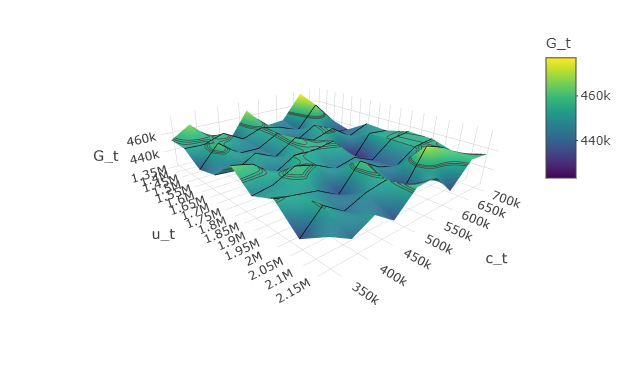
\includegraphics[width=6.25in,height=\textheight]{fig-analisis2pdf.png}
\end{center}

Se presenta también el análisis de sensibilidad para \(t = 19\), debido
a que en \(19\) semanas se presenta el caso donde se pueden registrar
ventas por debajo del cero, es decir, casos donde \(G(t)\leq0\).

\begin{Shaded}
\begin{Highlighting}[]
\FunctionTok{library}\NormalTok{(dplyr) }\CommentTok{\# libreria para poder }
\CommentTok{\# renombrar las cabeceras de los dataframes}

\CommentTok{\# Parametros}
\FunctionTok{set.seed}\NormalTok{(}\DecValTok{13}\NormalTok{) }\CommentTok{\#semilla fija}
\NormalTok{u }\OtherTok{=} \DecValTok{1759629} \CommentTok{\#surplus(capital inicial de salvamento)}
\CommentTok{\# Es un estimado a partir de la media de las ganancias por semana, }
\CommentTok{\# multiplicado por 10/3, }
\CommentTok{\# siendo una proporción para evitar la ruina}
\CommentTok{\# u (sum(medias))*(10/3)}
\NormalTok{decimal\_c }\OtherTok{=} \FloatTok{0.29}
\NormalTok{c }\OtherTok{=}\NormalTok{decimal\_c}\SpecialCharTok{*}\NormalTok{u }\CommentTok{\#prima de pago cada timepo t. c=0.5*u}
\NormalTok{lambda\_Nt }\OtherTok{=} \FloatTok{0.5}
\CommentTok{\#lambda\_Xi = 3}
\NormalTok{t\_final }\OtherTok{=} \DecValTok{19}
\CommentTok{\# S(t) = \textbackslash{}sum\_\{i=1\}\^{}\{N(t)\}X\_i}
\CommentTok{\# donde N(t)\textasciitilde{} Poisson (lambda*t)}
\CommentTok{\# X\_i \textasciitilde{} exponencial (lambda\_Xi)}
\CommentTok{\# CL = REPRESENTA EL MODELO DE CRAMER LUNDBERG}
\CommentTok{\# Simulación de trayectoria de CL\_t, cuando t \textless{} t\_final.}
\NormalTok{trayectoria\_CLt\_post\_pandemia }\OtherTok{\textless{}{-}} \ControlFlowTok{function}\NormalTok{(u, c, lambda\_Nt, t\_final)}
\NormalTok{\{}
\NormalTok{  tiempo }\OtherTok{\textless{}{-}} \FunctionTok{c}\NormalTok{(}\DecValTok{0}\NormalTok{)}
\NormalTok{  Cramer\_trayectoria }\OtherTok{\textless{}{-}} \FunctionTok{c}\NormalTok{(u)}
  \ControlFlowTok{while}\NormalTok{(tiempo[}\FunctionTok{length}\NormalTok{(tiempo)] }\SpecialCharTok{\textless{}}\NormalTok{ t\_final)}
\NormalTok{  \{}
    \CommentTok{\#tiempo\_llegada \textless{}{-} rexp(1, rate = lambda\_Nt)}
\NormalTok{    tiempo\_llegada }\OtherTok{\textless{}{-}}\NormalTok{ (}\DecValTok{1}\NormalTok{)}
\NormalTok{    Y\_i }\OtherTok{\textless{}{-}}\NormalTok{  (}\FunctionTok{rnorm}\NormalTok{(}\DecValTok{1}\NormalTok{, }\AttributeTok{mean =} \FloatTok{101919.050}\NormalTok{ , }\AttributeTok{sd =} \FloatTok{10877.075}\NormalTok{) }\SpecialCharTok{+} 
              \FunctionTok{rnorm}\NormalTok{(}\DecValTok{1}\NormalTok{, }\AttributeTok{mean =}  \FloatTok{39841.721}\NormalTok{ , }\AttributeTok{sd=} \FloatTok{7873.446}\NormalTok{)  }\SpecialCharTok{+}  
              \FunctionTok{rnorm}\NormalTok{(}\DecValTok{1}\NormalTok{, }\AttributeTok{mean =}   \FloatTok{41751.747}\NormalTok{, }\AttributeTok{sd =} \FloatTok{5687.030}\NormalTok{) }\SpecialCharTok{+} 
              \FunctionTok{rnorm}\NormalTok{(}\DecValTok{1}\NormalTok{, }\AttributeTok{mean =}   \FloatTok{43243.143}\NormalTok{, }\AttributeTok{sd =} \FloatTok{10517.841}\NormalTok{)}\SpecialCharTok{+} 
              \FunctionTok{rnorm}\NormalTok{(}\DecValTok{1}\NormalTok{, }\AttributeTok{mean =} \FloatTok{43010.307}\NormalTok{  , }\AttributeTok{sd =} \FloatTok{7741.889}\NormalTok{) }\SpecialCharTok{+} 
              \FunctionTok{rnorm}\NormalTok{(}\DecValTok{1}\NormalTok{, }\AttributeTok{mean =} \FloatTok{61191.300}\NormalTok{  , }\AttributeTok{sd =} \FloatTok{7202.989}\NormalTok{) }\SpecialCharTok{+} 
              \FunctionTok{rnorm}\NormalTok{(}\DecValTok{1}\NormalTok{, }\AttributeTok{mean =}  \FloatTok{85684.058}\NormalTok{ , }\AttributeTok{sd =} \FloatTok{8371.359}\NormalTok{)) }
\NormalTok{    tiempo }\OtherTok{\textless{}{-}} \FunctionTok{c}\NormalTok{(tiempo, tiempo[}\FunctionTok{length}\NormalTok{(tiempo)] }
                \SpecialCharTok{+}\NormalTok{ tiempo\_llegada,tiempo[}\FunctionTok{length}\NormalTok{(tiempo)] }
                \SpecialCharTok{+}\NormalTok{ tiempo\_llegada ) }
\NormalTok{    Cramer\_trayectoria }\OtherTok{\textless{}{-}} \FunctionTok{c}\NormalTok{(Cramer\_trayectoria,}
\NormalTok{                      Cramer\_trayectoria[}\FunctionTok{length}\NormalTok{(Cramer\_trayectoria)]}\SpecialCharTok{{-}} 
\NormalTok{                        c}\SpecialCharTok{*}\NormalTok{tiempo\_llegada, }
\NormalTok{                      Cramer\_trayectoria[}\FunctionTok{length}\NormalTok{(Cramer\_trayectoria)]}\SpecialCharTok{{-}} 
\NormalTok{                       c}\SpecialCharTok{*}\NormalTok{tiempo\_llegada }\SpecialCharTok{+}\NormalTok{  Y\_i )}
    \ControlFlowTok{if}\NormalTok{(Cramer\_trayectoria[}\FunctionTok{length}\NormalTok{(Cramer\_trayectoria)] }\SpecialCharTok{\textless{}} \DecValTok{0}\NormalTok{)}
\NormalTok{    \{}
\NormalTok{      ruina }\OtherTok{=} \DecValTok{1}
\NormalTok{    \}}
    \ControlFlowTok{else}
\NormalTok{    \{}
\NormalTok{      ruina }\OtherTok{=} \DecValTok{0}
\NormalTok{    \}}
\NormalTok{  \}}
\NormalTok{  df\_post\_pandemia}\OtherTok{\textless{}{-}} \FunctionTok{data.frame}\NormalTok{(tiempo, Cramer\_trayectoria)}
\NormalTok{  df\_trayectoria\_post\_pandemia }\OtherTok{\textless{}{-}} \FunctionTok{data.frame}\NormalTok{(df\_post\_pandemia}\SpecialCharTok{\%\textgreater{}\%}
                                  \FunctionTok{rename}\NormalTok{(}\AttributeTok{Tiempo =}\NormalTok{ tiempo, }
                                         \AttributeTok{Ct =}\NormalTok{ Cramer\_trayectoria))}
  \FunctionTok{return}\NormalTok{(df\_trayectoria\_post\_pandemia}\SpecialCharTok{$}\NormalTok{Ct[length}
\NormalTok{                                (df\_trayectoria\_post\_pandemia}\SpecialCharTok{$}\NormalTok{Ct)])}
\NormalTok{\}}

\CommentTok{\# La función generador\_mediana nos calcula la mediana de }
\CommentTok{\# las ganancias finales de 100 trayectorias, }
\CommentTok{\# fijando el u= surplus y el c}
\NormalTok{generador\_mediana\_post\_pandemia}\OtherTok{\textless{}{-}} \ControlFlowTok{function}\NormalTok{(ui,cj)}
\NormalTok{  \{}
\NormalTok{  ganancia\_final\_replicas\_post\_pandemia }\OtherTok{\textless{}{-}} \FunctionTok{replicate}\NormalTok{(}\DecValTok{100}\NormalTok{,}
           \FunctionTok{trayectoria\_CLt\_post\_pandemia}\NormalTok{(u, c,lambda\_Nt, t\_final))}
    \FunctionTok{return}\NormalTok{( }\FunctionTok{median}\NormalTok{(ganancia\_final\_replicas\_post\_pandemia))}
\NormalTok{  \}}
\CommentTok{\# Se crea la rejilla donde se hace el analisis de sensibilidad}
\CommentTok{\# para diferentes valores de u y c}
\NormalTok{grid\_u\_post\_pandemia }\OtherTok{\textless{}{-}} \FunctionTok{seq}\NormalTok{(}\AttributeTok{from =}\NormalTok{ (u}\DecValTok{{-}100000}\SpecialCharTok{*}\DecValTok{4}\NormalTok{), }
                            \AttributeTok{to =}\NormalTok{ (u}\SpecialCharTok{+}\DecValTok{100000}\SpecialCharTok{*}\DecValTok{4}\NormalTok{), }
                            \AttributeTok{by =} \DecValTok{100000}\NormalTok{)}
\NormalTok{grid\_c\_post\_pandemia }\OtherTok{\textless{}{-}} \FunctionTok{seq}\NormalTok{(}\AttributeTok{from =}\NormalTok{ (decimal\_c}\FloatTok{{-}0.01}\SpecialCharTok{*}\DecValTok{4}\NormalTok{), }
                            \AttributeTok{to =}\NormalTok{ (decimal\_c}\FloatTok{+0.01}\SpecialCharTok{*}\DecValTok{4}\NormalTok{), }
                            \AttributeTok{by =} \FloatTok{0.01}\NormalTok{)}
\NormalTok{u\_t }\OtherTok{\textless{}{-}}\NormalTok{ grid\_u\_post\_pandemia}
\NormalTok{matriz\_mediana\_post\_pandemia }\OtherTok{\textless{}{-}} \FunctionTok{matrix}\NormalTok{(}\FunctionTok{rep}\NormalTok{(}\DecValTok{0}\NormalTok{, }
      \FunctionTok{length}\NormalTok{(grid\_u\_post\_pandemia)}\SpecialCharTok{*}\FunctionTok{length}\NormalTok{(grid\_c\_post\_pandemia)),}
      \AttributeTok{nrow=} \FunctionTok{length}\NormalTok{(grid\_u\_post\_pandemia), }
      \AttributeTok{ncol=} \FunctionTok{length}\NormalTok{(grid\_c\_post\_pandemia))}

\NormalTok{G\_t }\OtherTok{\textless{}{-}}\NormalTok{ matriz\_mediana\_post\_pandemia}

\ControlFlowTok{for}\NormalTok{ (i }\ControlFlowTok{in} \DecValTok{1}\SpecialCharTok{:}\FunctionTok{length}\NormalTok{(u\_t)) }
\NormalTok{\{}
  \ControlFlowTok{for}\NormalTok{ (j }\ControlFlowTok{in} \DecValTok{1}\SpecialCharTok{:}\FunctionTok{length}\NormalTok{(grid\_c\_post\_pandemia)) }
\NormalTok{  \{}
\NormalTok{    G\_t[i,j] }\OtherTok{\textless{}{-}} \FunctionTok{generador\_mediana\_post\_pandemia}\NormalTok{(u\_t[i], }
\NormalTok{                                  grid\_c\_post\_pandemia[j]}\SpecialCharTok{*}\NormalTok{u\_t[i])}
\NormalTok{  \}}
\NormalTok{\} }

\CommentTok{\#Grafica del ánalisis de sensibilidad}
\CommentTok{\#Grafica del ánalisis de sensibilidad}
\FunctionTok{library}\NormalTok{(plotly)}
\FunctionTok{library}\NormalTok{(ggplot2)}
\NormalTok{c\_t }\OtherTok{\textless{}{-}}\NormalTok{ grid\_u\_post\_pandemia}\SpecialCharTok{*}\NormalTok{grid\_c\_post\_pandemia}

\NormalTok{z1}\OtherTok{\textless{}{-}} \FunctionTok{matrix}\NormalTok{(}\FunctionTok{rep}\NormalTok{(}\DecValTok{0}\NormalTok{,}
\FunctionTok{length}\NormalTok{(grid\_u\_post\_pandemia)}\SpecialCharTok{*}\FunctionTok{length}\NormalTok{(grid\_c\_post\_pandemia)), }\AttributeTok{nrow=}
\FunctionTok{length}\NormalTok{(grid\_u\_post\_pandemia), }\AttributeTok{ncol=} \FunctionTok{length}\NormalTok{(grid\_c\_post\_pandemia))}

\NormalTok{z2}\OtherTok{\textless{}{-}} \FunctionTok{matrix}\NormalTok{(}\FunctionTok{rep}\NormalTok{(u,}
\FunctionTok{length}\NormalTok{(grid\_u\_post\_pandemia)}\SpecialCharTok{*}\FunctionTok{length}\NormalTok{(grid\_c\_post\_pandemia)), }\AttributeTok{nrow=}
\FunctionTok{length}\NormalTok{(grid\_u\_post\_pandemia), }\AttributeTok{ncol=} \FunctionTok{length}\NormalTok{(grid\_c\_post\_pandemia))}

\NormalTok{fig3 }\OtherTok{\textless{}{-}} \FunctionTok{plot\_ly}\NormalTok{(}
  \AttributeTok{type =} \StringTok{\textquotesingle{}surface\textquotesingle{}}\NormalTok{,}
  \AttributeTok{contours =} \FunctionTok{list}\NormalTok{(}
    \AttributeTok{x =} \FunctionTok{list}\NormalTok{(}\AttributeTok{show =} \ConstantTok{TRUE}\NormalTok{, }\AttributeTok{start =}\NormalTok{ u\_t[}\DecValTok{1}\NormalTok{], }\AttributeTok{end =}
\NormalTok{u\_t[}\FunctionTok{length}\NormalTok{(u\_t)], }\AttributeTok{size =}\DecValTok{100000}\NormalTok{ ,}
\AttributeTok{color =} \StringTok{\textquotesingle{}black\textquotesingle{}}\NormalTok{),}
    \AttributeTok{z =} \FunctionTok{list}\NormalTok{(}\AttributeTok{show =} \ConstantTok{TRUE}\NormalTok{, }\AttributeTok{start =}\NormalTok{ G\_t[}\DecValTok{1}\NormalTok{], }
             \AttributeTok{end =}\NormalTok{ G\_t[}\FunctionTok{length}\NormalTok{(G\_t)], }\AttributeTok{size =}\FloatTok{0.01}\SpecialCharTok{*}\DecValTok{100000}\NormalTok{ , }
             \AttributeTok{color =} \StringTok{\textquotesingle{}white\textquotesingle{}}\NormalTok{)),}
  \AttributeTok{x =} \SpecialCharTok{\textasciitilde{}}\NormalTok{u\_t,}
  \AttributeTok{y =} \SpecialCharTok{\textasciitilde{}}\NormalTok{c\_t,}
  \AttributeTok{z =} \SpecialCharTok{\textasciitilde{}}\NormalTok{G\_t)}

\NormalTok{fig3 }\OtherTok{\textless{}{-}}\NormalTok{ fig3}\SpecialCharTok{\%\textgreater{}\%} \FunctionTok{add\_surface}\NormalTok{(}
  \AttributeTok{type =} \StringTok{\textquotesingle{}surface\textquotesingle{}}\NormalTok{,}
  \AttributeTok{contours =} \FunctionTok{list}\NormalTok{(}
    \AttributeTok{x =} \FunctionTok{list}\NormalTok{(}\AttributeTok{show =} \ConstantTok{TRUE}\NormalTok{, }\AttributeTok{start =}\NormalTok{ u\_t[}\DecValTok{1}\NormalTok{], }
             \AttributeTok{end =}\NormalTok{ u\_t[}\FunctionTok{length}\NormalTok{(u\_t)], }\AttributeTok{size =}\DecValTok{100000}\NormalTok{ ,}
             \AttributeTok{color =} \StringTok{\textquotesingle{}black\textquotesingle{}}\NormalTok{),}
    \AttributeTok{y =} \FunctionTok{list}\NormalTok{(}\AttributeTok{show =} \ConstantTok{TRUE}\NormalTok{, }\AttributeTok{start =}\NormalTok{ c\_t[}\DecValTok{1}\NormalTok{], }
             \AttributeTok{end =}\NormalTok{ c\_t[}\FunctionTok{length}\NormalTok{(c\_t)], }
             \AttributeTok{size =} \FloatTok{0.01}\SpecialCharTok{*}\DecValTok{100000}\NormalTok{ , }\AttributeTok{color =} \StringTok{\textquotesingle{}red\textquotesingle{}}\NormalTok{)),}
  \AttributeTok{x =} \SpecialCharTok{\textasciitilde{}}\NormalTok{u\_t,}
  \AttributeTok{y =} \SpecialCharTok{\textasciitilde{}}\NormalTok{c\_t,}
  \AttributeTok{z =} \SpecialCharTok{\textasciitilde{}}\NormalTok{z1)}

\NormalTok{fig3 }\OtherTok{\textless{}{-}}\NormalTok{ fig3 }\SpecialCharTok{\%\textgreater{}\%} \FunctionTok{layout}\NormalTok{(}
  \AttributeTok{scene =} \FunctionTok{list}\NormalTok{(}
    \AttributeTok{xaxis =} \FunctionTok{list}\NormalTok{(}\AttributeTok{nticks =} \DecValTok{20}\NormalTok{),}
    \AttributeTok{zaxis =} \FunctionTok{list}\NormalTok{(}\AttributeTok{nticks =} \DecValTok{4}\NormalTok{),}
    \AttributeTok{camera =} \FunctionTok{list}\NormalTok{(}\AttributeTok{eye =} \FunctionTok{list}\NormalTok{(}\AttributeTok{x =} \DecValTok{0}\NormalTok{, }\AttributeTok{y =} \SpecialCharTok{{-}}\DecValTok{1}\NormalTok{, }\AttributeTok{z =} \DecValTok{1}\NormalTok{)),}
    \AttributeTok{aspectratio =} \FunctionTok{list}\NormalTok{(}\AttributeTok{x =}\NormalTok{ .}\DecValTok{9}\NormalTok{, }\AttributeTok{y =}\NormalTok{ .}\DecValTok{8}\NormalTok{, }\AttributeTok{z =} \FloatTok{0.2}\NormalTok{)))}


\NormalTok{fig3}
\end{Highlighting}
\end{Shaded}

\begin{center}
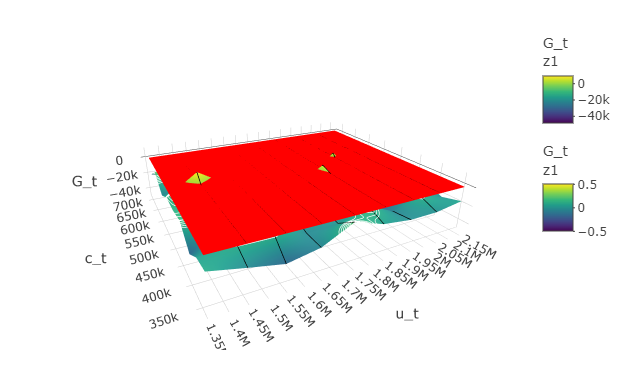
\includegraphics[width=6.25in,height=\textheight]{fig-analisis3pdf.png}
\end{center}

\section{Análisis de resultados y
recomendaciones.}\label{anuxe1lisis-de-resultados-y-recomendaciones.}

Con los datos registrados de \(90\) semanas antes de pandemia en el
modelo modificado (Ecuación~\ref{eq-4.1pdf}) se obtiene un crecimiento
positivo de las ganancias simuladas, en particular mayor que el capital
inicial, es decir la probabilidad del evento donde \(G(t)\geq u\) es
positiva, con \(t=90\), como se puede observar en la imagen
(Figura~\ref{fig-fig-trayectoriapdf}), por lo que en el intervalo de
tiempo en el que se estudia la empresa generaría siempre ganancias
positivas y se lograría suplir la deuda e incluso pensar en implementar
más equipos inmobiliarios.

Mientras que después de la pandemia, se puede argumentar con base en las
observaciones de las \(14\) semanas de las ventas registradas, usando
los mismos parámetros obtenidos para los datos antes de la pandemia
implementados, las ganancias son bajas como se muestra en la imagen
(Figura~\ref{fig-fig-trayectoria2pdf}). Aquí se observa que la
simulación de las ganancias son menores que el capital inicial y al dar
seguimiento en el intervalo de tiempo con los datos registrados después
de pandemia hasta la semana \(17\) se observa que las ganancias son
menores que cero, por lo que se puede concluir que se llega a una ruina
total, como se muestra el caso en la imagen
(Figura~\ref{fig-fig-trayectoria3pdf}).

Analizando el caso en el que se modifica los parámetros de los costos
del modelo (Ecuación~\ref{eq-4.1pdf}) , se concluye que al calibrar el
parámetro \(c\), este se puede reducir a un \(17 \%\) para cuando
\(t=14\), es decir, al final de la semana \(14\) puede evitarse la
perdida total de las ganancias que son mayores que el capital inicial,
como se observa en la figura (\textbf{?@fig-fig-trayectoria4pdf}).

Como \(c\), es el parámetro de los pagos que incluye el pago de la
adquisición de la franquicia, compras de equipos inmobiliarios, pagos de
empleados y prestamos, el anterior análisis quiere decir que se necesita
un recorte de personal del \(17 \%\) como mínimo y una reestructuración
financiera del capital pendiente por pagar, haciendo los pagos más
pequeños a un tiempo extendido, con el fin de la funcionalidad del
negocio durante este proceso pandemico y evitar el cierre de quiebra.

\bookmarksetup{startatroot}

\chapter*{Referencias}\label{referencias}
\addcontentsline{toc}{chapter}{Referencias}

\markboth{Referencias}{Referencias}

\phantomsection\label{refs}
\begin{CSLReferences}{1}{0}
\bibitem[\citeproctext]{ref-castaneda2012introduction}
Castañeda, Liliana Blanco, Viswanathan Arunachalam, y Selvamuthu
Dharmaraja. 2012. \emph{Introduction to probability and stochastic
processes with applications}. John Wiley \& Sons.

\bibitem[\citeproctext]{ref-wickham2023r}
Wickham, Hadley, Mine Çetinkaya-Rundel, y Garrett Grolemund. 2023.
\emph{R for data science}. " O'Reilly Media, Inc.".

\end{CSLReferences}



\end{document}
